\documentclass{article}

\usepackage{multirow}
\usepackage{amsmath, amsthm, amssymb, amsfonts}
\usepackage{thmtools}
\usepackage{graphicx}
\usepackage{setspace}
\usepackage{geometry}
\usepackage{float}
\usepackage[colorlinks=true, linkcolor=blue, citecolor=red, urlcolor=blue]{hyperref}
\usepackage[utf8]{inputenc}
\usepackage[english]{babel}
\usepackage{framed}
\usepackage[dvipsnames]{xcolor}
\usepackage{tcolorbox}
\usepackage{listings}
\usepackage{minted}
% s\usepackage{booktabs}
\usepackage{capt-of}
\usepackage{tikz}
\usepackage{mathrsfs}
\usepackage{enumitem} % for customizing enumerate
\usetikzlibrary{decorations.pathreplacing}
\usepackage{tikz-3dplot}

\usepackage{pgfplots}
\pgfplotsset{compat=1.18}
\usetikzlibrary{arrows.meta,positioning,decorations.pathreplacing}
\usetikzlibrary{backgrounds} % Simplified library requirements



\theoremstyle{plain}
\newtheorem{thm}{Theorem}[section]
\newtheorem{lem}[thm]{Lemma}
\newtheorem{cor}[thm]{Corollary}

\theoremstyle{definition}
\newtheorem{defn}[thm]{Definition}
\newtheorem*{ex}{Example}
\newtheorem{prop}[thm]{Proposition}

\DeclareMathOperator{\diam}{diam}

\theoremstyle{remark}
\newtheorem*{rem}{Remark}

\colorlet{LightGray}{White!90!Periwinkle}
\colorlet{LightOrange}{Orange!15}
\colorlet{LightGreen}{Green!15}

\newcommand{\HRule}[1]{\rule{\linewidth}{#1}}

\declaretheoremstyle[name=Theorem,]{thmsty}
\declaretheorem[style=thmsty,numberwithin=section]{theorem}
\tcolorboxenvironment{theorem}{colback=LightGray}

\declaretheoremstyle[name=Proposition,]{prosty}
\declaretheorem[style=prosty,numberlike=theorem]{proposition}
\tcolorboxenvironment{proposition}{colback=LightOrange}

\declaretheoremstyle[name=Principle,]{prcpsty}
\declaretheorem[style=prcpsty,numberlike=theorem]{principle}
\tcolorboxenvironment{principle}{colback=LightGreen}

\setstretch{1.2}
\geometry{
    textheight=9.5in,
    textwidth=7in,
    top=0.75in,
    headheight=12pt,
    headsep=25pt,
    footskip=30pt
}

\usepackage{enumitem}
\newcommand{\subscript}[2]{$#1 _ #2$}

% ------------------------------------------------------------------------------

\begin{document}

% ------------------------------------------------------------------------------
% Cover Page and ToC
% ------------------------------------------------------------------------------

\begin{center}
  % line length = 209pt = 13 * 19 (length of "Binary Search Trees")
  \rule[0pt]{\textwidth}{1.5pt} \\ ~\\
		\Huge {{\textbf{Self-Similarity and Fractals}} } \\  % title 
  \rule[0pt]{\textwidth}{1.5pt} 
  \end{center} % Large text is 11pt, so 
  
   ~\\ ~\\ ~\\ ~\\ ~\\ ~\\
		% \HRule{1.5pt} \\  

   %  \noindent\rule{\linewidth}{.6pt}
    \begin{figure}[hbt!]
    \centering
        \centering
        \includegraphics[width=0.4\textwidth]{assets/uct.png} % Path to the second image
        
        \label{fig:acf}
    
\end{figure}
   ~\\ ~\\ ~\\ ~\\ ~\\ ~\\
   \begin{center}
   \large {Author:} \large{ {Alexander Cristaudo}} \\
    \large{Supervisor:} \large{ Dr Francois Ebobisse} \\ 
    \large {Department of Mathematics and Applied Mathematics} \\
    \large {Date: 03 October 2025}
   \end{center}



\newpage

\section*{Preface}
This thesis investigates the geometry of certain mathematical shapes through analytical tools. In particular, it focuses on Hausdorff metrics, Hausdorff measures, and their applications to self-similar structures and fractals, with the aim of understanding how to calculate the sizes and dimensions of these intricate regions. My motivation for choosing this topic comes from a long-standing fascination with infinitely complex figures, especially fractals. Though they often arise from simple recursive rules, their geometry resists description by standard methods in measure theory, which makes them both challenging and captivating to study.
~\\~\\
Fractals, as a mathematical concept, have a rich history that blends geometry and analysis. While the term \textit{fractal} does not have one agreed upon definition, it was initially introduced by Benoît B. Mandelbrot in 1975 (as a some set whose Hausdorff dimension exceeds its topological dimension), who is often regarded as the father of fractal geometry. His work demonstrated how irregular and fragmented shapes in nature, such as coastlines, clouds and mountains, can be described using mathematical structures that repeat at different scales. He is also known for his construction of the Mandelbrot set, a fractal famous for its complex mathematical description and visual complexity. 
~\\~\\
Further contributions arose in the early twentieth century from Gaston Julia (famous for 'Julia Sets') and Pierre Fatou. They investigated iterating rational functions in the complex plane and realised fractal structures appear with certain functions. Felix Hausdorff devised a way to measure these sets: the Hausdorff measure. This extends classical notions of length, area, and volume, giving us the tools to assign “sizes” to sets with highly irregular geometry.
~\\~\\
This, paired with the Hausdorff metric, which offers a natural way to compare distances between sets and provides a rigorous framework for understanding convergence of geometric structures, open up a powerful way to study and analyse self-similar objects.
~\\ ~\\
Mandelbrot's work in the latter half of the twentieth century unified these strands of research into what is now known as fractal geometry.
Several of the most well-known examples of fractal sets are named after the mathematicians who first introduced them. The Cantor set, defined by Georg Cantor in the late nineteenth century, arises from the iterative removal of middle thirds from a closed interval and represents one of the earliest constructions of a totally disconnected, uncountable set. The Koch snowflake, introduced by Helge von Koch in 1904, is obtained by repeatedly modifying the sides of an equilateral triangle to form a boundary of infinite length contained within a finite area. The Sierpiński triangle and the Sierpiński carpet, both due to Wacław Sierpiński in the early twentieth century, are planar fractals constructed through recursive removal of triangular and square subsets, respectively. These classical examples illustrate the diversity of fractal geometry and serve as examples of self-similarity and infinite complexity.
~\\~\\
In the chapters that follow, I outline the theoretical background behind these constructions, explore their role in classical fractals, and emphasise the central part played by self-similarity in their geometry. My aim is to demonstrate how the abstract definitions of the Hausdorff metric and measure lead not only to elegant mathematics but also to deeper insights into the structure of irregular sets.
~\\~\\
This thesis represents the culmination of my Honours research project. I am sincerely grateful to my supervisor, Dr. Francois Ebobisse, for his guidance, recommendations, and encouragement throughout. His expertise has shaped my approach to mathematics and greatly enriched the work presented here.

\newpage

\tableofcontents  % generates the table of contents
\newpage 


\section{Plagiarism Declaration}
\begin{enumerate}
    \item I know that plagiarism is a serious form of academic dishonesty.
    \item I have read the document about avoiding plagiarism, am familiar with its contents and have avoided all forms of plagiarism mentioned there.
    \item Where I have used the words of others, I have indicated this by the use of quotation marks. 
    \item I have referenced all quotations and other ideas borrowed from others.
    \item I have not and shall not allow others to plagiarise my work. 
\end{enumerate}
Signature: ~\\

\includegraphics[scale = 0.5]{assets/sign.png}
\newpage

% \section{Preface}
% \newpage 

\section{Preliminaries}

\subsection*{Notation}
We fix the following notational conventions throughout this thesis:
\begin{itemize}
  \item $\mathbb{N}^+ = \{1,2,3,\dots\}$ the set of positive integers,
  \item $\mathbb{N}_0 = \{0,1,2,\dots\}$ the set of natural numbers with zero (the nonnegative integers),
  \item $\mathbb{R}$ the set of real numbers,
  \item $\overline{\mathbb{R}} = \mathbb{R}\cup\{-\infty,+\infty\}$ the extended real line,
  \item $\overline{\mathbb{R}}_+ = [0, \infty) \cup \{\infty\}$ the nonnegative extended reals,
  \item $\lambda_n$ denotes the $n$-dimensional Lebesgue measure,
\end{itemize}

\subsection*{A Preliminary Inequality}
\begin{thm} \label{thm:sub}
Let $(f_n)_{n \in \mathbb{N}^+}$ be a sequence of nonnegative functions $f_n:A\to \overline{\mathbb{R}}^+$. Then
\[
\sup_{a\in A}\,\sum_{n=1}^\infty f_n(a) \;\le\; \sum_{n=1}^\infty \sup_{a\in A} f_n(a).
\]
\end{thm}
\begin{proof}
For any fixed $a\in A$,
\[
\sum_{n=1}^\infty f_n(a) \;\le\; \sum_{n=1}^\infty \sup_{a\in A} f_n(a).
\]
This sum converges (possibly to infinity). Taking the supremum over $a\in A$ yields the desired inequality.
\end{proof}

\subsection*{Metric Spaces and Topology}
\begin{defn}[Metric Space]
A \emph{metric space} is a pair $(X,d)$ where $X$ is a set and $d:X\times X\to\mathbb R$ is a distance function satisfying for all $x,y,z\in X$: 
\[
d(x,y)\ge 0,\quad d(x,y)=0\iff x=y,\quad d(x,y)=d(y,x),\quad d(x,z)\le d(x,y)+d(y,z).
\] 
\end{defn}

\begin{defn}[Open and Closed Balls]
In a metric space $(X,d)$, for any point $x\in X$ and radius $r>0$ the \emph{open ball} is defined by 
\[
B(x;r)=\{y\in X: d(x,y)<r\},
\] 
and the \emph{closed ball} by 
\[
\overline B(x;r)=\{y\in X: d(x,y)\le r\}.
\] 
\end{defn}

\begin{defn}[Open set]
Let $(X,d)$ be a metric space. A subset $U \subseteq X$ is called \emph{open} if for every $x \in U$ there exists $r>0$ such that 
\[
B(x;r) := \{ y \in X : d(x,y) < r \} \subseteq U.
\]
\end{defn}

\begin{defn}[Closed set]
A subset $F \subseteq X$ is called \emph{closed} if its complement $X \setminus F$ is open. 
Equivalently, $F$ is closed if every convergent sequence $(x_n)$ in $F$ with limit $x \in X$ satisfies $x \in F$.
\end{defn}


\begin{defn}[Diameter]
If $E\subseteq X$ is a bounded subset, its \emph{diameter} is 
\[
\diam(E)=\sup\{d(x,y): x,y\in E\}.
\] 
\end{defn}

\begin{defn}[Compactness]
A metric space $X$ is \emph{compact} if every open cover of $X$ has a finite subcover. Equivalently (in metric spaces), $X$ is compact if every sequence in $X$ has a convergent subsequence whose limit lies in $X$. 
\end{defn}

\begin{defn}[Completeness]
A metric space $(X,d)$ is \emph{complete} if every Cauchy sequence in $X$ converges to a limit in $X$. 
\end{defn}

\begin{defn}[Separability]
A metric space $X$ is \emph{separable} if there exists a countable dense subset $D\subset X$ (for example, $\mathbb Q$ is dense in $(\mathbb R,|\cdot|)$). 
\end{defn}
Every Euclidean space $\mathbb{R}^n$ with the usual metric is separable, since $\mathbb{Q}^n$ is dense. 
In this thesis we will only work with subsets of $\mathbb{R}^n$, so separability is automatic and not used explicitly in later sections.

\begin{defn}
A topological space $X$ is \emph{connected} if there do not exist nonempty disjoint open sets $U,V\subset X$ with $U\cup V = X$. Equivalently, the only subsets of $X$ that are both open and closed are $\emptyset$ and $X$. A subset $A\subset X$ is said to be connected if it is connected in the subspace topology.
\end{defn}

\begin{defn}[Totally disconnected space]
A topological space $X$ is called \emph{totally disconnected} if the only connected subsets of $X$ are singletons. 
\end{defn}


\subsection*{Contraction Mappings and Fixed Points}
\begin{defn}[Contraction Mapping]
Let $(X,d)$ be a metric space. A map $f:X\to X$ is called a \emph{contraction} if there exists a constant $c\in[0,1)$ such that 
\[
d(f(x),f(y))\le c\,d(x,y)\quad\forall x,y\in X.
\] 
The number $c$ is called a \emph{Lipschitz constant} for $f$ 
\end{defn}

\begin{defn}[Fixed Point]
A point $x\in X$ is a \emph{fixed point} of a map $f:X\to X$ if $f(x)=x$
\end{defn}

\begin{thm}[Banach Fixed Point / Contraction Mapping Theorem]
Let $(X,d)$ be a non-empty complete metric space and $f:X\to X$ a contraction mapping. Then $f$ has a unique fixed point $x^* \in X$. Moreover, for any initial point $x_0\in X$ the iterates $x_{n+1}=f(x_n)$ converge to $x^*$ as $n\to\infty$ 
\end{thm}

\subsection*{Additional Results}
\begin{thm}\label{thm:gamma}
    Define the gamma function \[
    \Gamma (t):= \int \limits _0 ^\infty e^{-x}x^{t-1}dx
    \]
    Then $\Gamma (x+1) = x \Gamma (x)$.
\end{thm}

\subsection*{Measure Theory Basics}

\begin{defn}[$\sigma$-algebra]
Let $X$ be a set. A collection $\mathcal{A}\subseteq\mathcal{P}(X)$ is called a \emph{$\sigma$-algebra} if:
\begin{enumerate}
  \item $X\in\mathcal{A}$,
  \item If $A\in\mathcal{A}$, then $A^c\in\mathcal{A}$,
  \item If $(A_n)_{n=1}^\infty \subseteq \mathcal{A}$, then $\bigcup_{n=1}^\infty A_n \in \mathcal{A}$.
\end{enumerate}
\end{defn}

\begin{defn}[Measure]
Let $X$ be a set and $\mathcal{A}$ a $\sigma$-algebra on $X$. A function $\mu:\mathcal{A}\to [0,\infty]$ is called a \emph{measure} if:
\begin{enumerate}
  \item $\mu(\varnothing)=0$,
  \item For disjoint sets $A_1,A_2,\dots \in \mathcal{A}$,
  \[
  \mu\Bigl(\bigcup_{n=1}^\infty A_n\Bigr) \;=\; \sum_{n=1}^\infty \mu(A_n).
  \]
\end{enumerate}
\end{defn}

\begin{defn}[Measure space]
A triple $(X,\mathcal{A},\mu)$ is called a \emph{measure space}, where $X$ is a set, $\mathcal{A}$ is a $\sigma$-algebra of subsets of $X$, and $\mu$ is a measure on $\mathcal{A}$.
\end{defn}

\begin{defn}[Outer measure]
An \emph{outer measure} on $X$ is a function $\mu^*:\mathcal{P}(X)\to[0,\infty]$ such that:
\begin{enumerate}
  \item $\mu^*(\varnothing)=0$,
  \item If $A\subseteq B$, then $\mu^*(A)\le \mu^*(B)$ (monotonicity),
  \item For any sequence $(A_n)$,
  \[
  \mu^*\Bigl(\bigcup_{n=1}^\infty A_n\Bigr) \;\le\; \sum_{n=1}^\infty \mu^*(A_n)
  \quad\text{(countable subadditivity)}.
  \]
\end{enumerate}
\end{defn}

\begin{defn}[Carathéodory measurability]
If $\mu^*$ is an outer measure, a set $E\subseteq X$ is \emph{$\mu^*$-measurable} if for all $A\subseteq X$,
\[
\mu^*(A) = \mu^*(A\cap E) + \mu^*(A\cap E^c).
\]
\end{defn}

\begin{thm}[Carathéodory's Theorem] \label{thm:caratheodory}
Let $\mu^*$ be an outer measure on $X$. Then the collection of $\mu^*$-measurable sets is a $\sigma$-algebra, and the restriction of $\mu^*$ to this $\sigma$-algebra is a complete measure.
\end{thm}

\begin{thm}[Tonelli's Theorem for sums]
\label{thm:tonelli-sums}
Let $(a_{m,n})_{m,n\in\mathbb{N}_0}$ be a doubly-indexed family of nonnegative extended real numbers, i.e.\ $a_{m,n}\in [0,\infty]$. Then
\[
\sum_{m=0}^\infty\sum_{n=0}^\infty a_{m,n}
= \sum_{n=0}^\infty\sum_{m=0}^\infty a_{m,n}
= \sup_{F\subseteq \mathbb{N}_0\times \mathbb{N}_0 \atop F \text{ finite}}
     \;\sum_{(m,n)\in F} a_{m,n} =: \sum \limits _{(m,n) \in \mathbb{N}_0 \times \mathbb{N}_0} a_{m,n}
\]
In particular, both sums exist in $[0,\infty]$ and are equal to the double series.
\end{thm}

\begin{defn}
The $n$-dimensional Lebesgue measure $\lambda_n$ on $\mathbb{R}^n$ is the unique $\sigma$-finite measure such that \[
\lambda _n \left ( \prod_{i=1}^n (a_i, b_i] \right)= \prod \limits _{i=1} ^n \max \{b_i-a_i, 0 \}
\]
\end{defn}


\newpage 

\section{The Hausdorff Metric}
\subsection{Motivation and Initial Challenges}
Let $(X,d)$ be a metric space. Recall that for sets $A,B \subseteq X$
\begin{center}
    $d(x,B) := \inf \limits _{b \in B}d(x,b)$  \\ ~\\
    $d(A,B):=\sup \limits _{a \in A}d(a,B) = \sup \limits _{a \in A}  \inf \limits _{b \in B} d(a,b)$\\ ~\\
    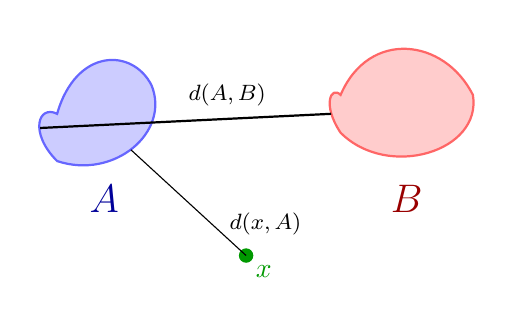
\begin{tikzpicture}[scale=1.2]

  % Set A - blue blob
  \fill[blue!20, draw=blue!60, thick]
    (0,0) 
    .. controls (0.2,0.7) and (0.8,0.7) .. (1,0.3)
    .. controls (1.2,-0.2) and (0.6,-0.7) .. (0,-0.5)
    .. controls (-0.3,-0.2) and (-0.2,0.1) .. (0,0)
    -- cycle;
  \node[blue!60!black] at (0.5,-0.9) {\Large $A$};

  % Set B - red blob
  \fill[red!20, draw=red!60, thick]
    (3,0.2) 
    .. controls (3.3,0.9) and (4.1,0.8) .. (4.4,0.2)
    .. controls (4.5,-0.4) and (3.5,-0.7) .. (3,-0.2)
    .. controls (2.8,0.1) and (2.9,0.3) .. (3,0.2)
    -- cycle;
  \node[red!60!black] at (3.7,-0.9) {\Large $B$};

  % Point x
  \filldraw[green!60!black] (2,-1.5) circle (2pt) node[below right] {$x$};

  % Dashed arrow from x to closest point in A
  \coordinate (a_closest) at (0.78,-0.38);
  \draw[] (2,-1.5) -- (a_closest) node[midway, below right] {\footnotesize $\ \ \ \ d(x,A)$};

  % Sample points in A
  \coordinate (a1) at (-0.18, -0.15);

  % Sample points in B
  \coordinate (b1) at (2.9, 0);


  % Dotted arrows from A to B
  \draw[thick, black] (a1) -- (b1);

  % Label for d(A,B)
  \node[black] at (1.8,0.2) {\footnotesize $d(A,B)$};

\end{tikzpicture}
\end{center}
The graphic above is a depiction in the metric space $(\mathbb{R}^2, d_E)$. We have that $d(x,A)$ is the minimum distance from a point $x$ to our set $A$, while for two sets $A$ and $B$, $d(A,B)$ is the supremum of distances from points in $A$ to the closest point in $B$. While $d(A,B)$ appears to be a natural choice to measure how close sets are, there are three problems. 
\begin{enumerate}
    \item This distance can be unbounded for infinite sets
    \item This distance is dependent on what set is first (i.e., in general, $d(A,B) \ne d(B,A)$)
    \item The empty set provides further extreme cases
\end{enumerate}
To see (1) and (2), consider the following example:
\begin{ex}
    We will consider the real numbers with the usual metric.
    \begin{center}
        $d(\{0\}, \mathbb{N}^+) = \sup \limits _{a \in \{0\}} \inf \limits _{n\in \mathbb{N}^+} |a-n| = \inf \limits _{n \in \mathbb{N}^+} n = 1$
    \end{center}
    On the other hand,
    \begin{center}
        $d(\mathbb{N}^+, \{0\}) = \sup \limits _{n \in \mathbb{N}^+} \inf \limits _{a\in \{0\}} |a-n| = \sup \limits _{n \in \mathbb{N}^+} n = \infty$
    \end{center}
\end{ex}
~\\ The empty set scenarios mentioned in (3) are:
\begin{ex}
    Let $(X,d)$ be a metric space, $x \in X$ and $\emptyset \ne  A \subseteq X$
    \begin{center}
        $d(x,\emptyset)=\inf \emptyset = \infty$ \\
        $d(\emptyset, A)=\sup \emptyset = -\infty$ \\
        $d(A, \emptyset) = \sup \limits _{a\in A} \inf \emptyset = \infty$   
    \end{center}
\end{ex}

~\\ Since we do not want infinite values, we must exclude empty sets as our solution to (3). To handle problem (1) - unbounded distance - we need to first establish some technical results about infima and suprema.
\begin{lem}\label{lem:infs}
    Let $f,g: X \to \mathbb{R}$ and $A\subseteq X$. Then $\left |\inf \limits _{a \in A}f(a) - \inf \limits _{a \in A}g(a) \right | \le \sup \limits _{a\in A}\left |f(a) - g(a) \right |$ 
\end{lem}
\begin{proof}
    Let $r = \sup \limits _{a\in A} \left |f(a) - g(a) \right |$ and $a\in A$.  Then $|f(a) - g(a)| \le r \iff g(a)-r\le f(a) \le g(a)+r$. Taking the infimum on both sides, we get $\inf \limits _{a\in A} g(a) - r\le \inf \limits _{a\in A} f(a) \le \inf \limits _{a\in A}g(a)+r \iff \left |\inf \limits _{a\in A}f(a) - \inf \limits _{a\in A}g(a) \right | \le r$ as required
\end{proof}
\begin{lem}\label{lem:well-defined}
    If $A\ne \emptyset$ is compact and $B$ is nonempty, then $d(A,B) < \infty$
\end{lem}
\begin{proof}
    Let $a \in A$ and define $f(a) :=\inf \limits _{b\in B} d(a,b)$. Since $B$ is nonempty, there is some $b' \in B$, and since $d$ is a metric, $0\le d(a,b')<\infty$ so $0\le f(a)<\infty$. Now $f$ is Lipschitz, since, using Lemma~\ref{lem:infs},
    \[|f(x)-f(y)| = \left |\inf \limits _{b \in B}d(x,b) - \inf \limits _{b \in B}d(y,b) \right |\le \sup \limits _{b\in B}\underbrace{|d(x,b) -d(y,b)|} \limits _{\le d(x,y) + d(b,b)} \le d(x,y)\] and is thus continuous. Then by the Extreme Value Theorem, $f$ attains a maximum $y<\infty$ and $d(A,B) = y$
\end{proof}
~\\ So, if we consider only the non-empty compact subsets of $X$, then each $d(A,B)$ for $A,B \subseteq X$ will be finite. We will denote the set of non-empty compact sets by $\mathcal{K}(X)$. That is, $\mathcal{K}(X) := \{A \subseteq X: A \text { is compact and } A\ne \emptyset\}$. The final problem is (2), and our solution is to choose the larger of $d(A,B)$ and $d(B,A)$ as our metric value. As a motivator as to why we choose the larger value, notice that, using the standard metric on $\mathbb{R}$, \[
d \left ([0,1], [0,2] \right ) = 0, \quad d([0,2], [0,1]) = 1, \quad [0,1] \ne [0,2]
\]
So choosing the smaller value cannot result in a metric. This is then what we define as the Hausdorff metric. Before proving it is indeed a metric, let's look at a few properties of these new function operations.

\begin{thm}\label{thm:d_properties}
    \begin{enumerate}
        For $A,B,C \in \mathcal{K}(X)$,  any set $D\subseteq X$ and $x \in X$
        \item $d(x,D)=0 \iff x\in \overline{D}$
        \item $d(A,B)=0 \iff A \subseteq B$
        \item There exists some $a_x \in A$ such that $d(x, A) = d(x, a_x)$
        \item There exists some $a\in A$ and $b\in B$ such that $d(A,B)=d(a,b)$
        \item $d(A,C) \le d(A,B) + d(B,C)$
    \end{enumerate}
\end{thm}

\begin{proof} $ $
    \begin{enumerate} 
        \item First suppose that $x \in \overline{D}$. Then there exists a sequence $(x_n)_{n\in \mathbb{N}}$ in $D$ such that $x_n \to x$ as $n\to \infty$. For $\varepsilon>0$, there is some $N_\varepsilon \in \mathbb{N}$ such that $d(x_{N_\varepsilon}, x) < \varepsilon$. Then $0 \le d(x,D) < \varepsilon$ and so $d(x, D)=0$. On the other hand, suppose $d(x,D) = 0$. Then, for any $n\in \mathbb{N}^+$, there is some $x_n \in D$ such that $d(x,x_n)< \frac{1}{n}$. Then $x_n \to x$ as $n \to \infty$ so $x \in \overline{D}$
        \item $d(A,B) = 0 \iff \sup \limits _{a \in A}  d(a,B) = 0$. Since $d(a,B) \ge 0$, $d(A,B)=0\iff d(a,B)=0 $ for all $ a \in A \iff a \in \overline{B}$ (by 1) for all $a \in A \iff A \subseteq \overline{B}$. But $B$ being compact means it is closed and so $d(A,B)=0 \iff A\subseteq B$
        \item For each $n\in \mathbb{N}^+$, there is some $x_n \in A$ such that $d(x_n, x)<d(x,A) + \frac{1}{n}$. Clearly $d(x, x_n) \to d(x,A)$ as $n\to \infty$. Now $(x_n)$ is a sequence in the compact set $A$, so there exists a subsequence $(x_{n_k})$ that converges to $a_x \in A$. Then, since the distance function is continuous, $d(x, a_x) = d \left (x, \lim \limits _{k\to \infty}x_{n_k} \right ) = \lim \limits _{k \to \infty}d(x,x_{n_k})=d(x,A)$.
        \item For each $n \in \mathbb{N}^+$, there exists some $a_n \in A$ such that $d(a_n, B)>d(A,B)-\frac{1}{n}$. By (3), there is some $b_n \in B$ such that $d(a_n, B) = d(a_n, b_n)$. We then have that $d(a_n, b_n) \to d(A,B)$ as $n \to \infty$. Since $A$ and $B$ are compact, there are converging subsequences $a_{n_k} \to a \in A$ and $b_{n_m} \to b \in B$ as $k,m \to \infty$. Then, using joint continuity of the distance function, $d(A,B) = \lim \limits _{k,m \to \infty}d(a_{n_k}, b_{n_m}) = d(a,b)$

        \item For any $a\in A$, by (3), there exists some $b_a\in B$ such that $d(a,B)=d(a,b_a)$. We have that \[d(a, C) = \inf \limits _{c\in C}d(a,c)\le \inf \limits _{c\in C}  \bigg [d(a, b_a)+d(b_a, c) \bigg] = d(a,b_a)+\inf \limits _{c\in C} d(b_a, c)=d(a,B)+d(b_a, C)\le d(A,B)+d(B,C)\]So $d(A,C) \le d(A,B) + d(B,C)$
    \end{enumerate}
\end{proof}

\subsection{Construction of the Hausdorff Metric}

\begin{thm}
    Let $(X,d)$ be a metric space. The function $d_H:\mathcal{K}(X) \to \mathbb{R} $ defined by $d_H(A,B) = \max \{d(A,B), d(B,A)\}$ is a metric on $\mathcal{K}(X)$
\end{thm}
\begin{proof} Lemma~\ref{lem:well-defined} shows $d_H$ is well-defined. Let $A,B,C \in \mathcal{K}(X)$
\begin{enumerate}[label=(MS\arabic*)]
    \item We have $d_H(A,B) = 0 \iff \max \{d(A,B), d(B,A)\}=0 \iff d(A,B)=d(B,A)=0$. From Theorem~\ref{thm:d_properties}\textcolor{blue}{.2}, $d(A,B)=0\iff A\subseteq B$ and $d(B,A)=0 \iff B\subseteq A$ so $d_H(A,B) = 0 \iff A=B$
    
    \item $d_H(A,B) = \max \{d(A,B), d(B,A)\} = \max \{d(B,A), d(A,B)\} = d_H(B,A)$

    \item $d_H(A,C) = \max \{d(A,C), d(C,A)\}$. Without loss of generality, assume $d(A,C) \ge d(C,A)$. Then, using Theorem~\ref{thm:d_properties}\textcolor{blue}{.5}, $d_H(A,C) = d(A,C) \le d(A,B) + d(B,C) \le d_H(A,B) + d_H(B,C)$. 
\end{enumerate}
\end{proof}

\noindent\fbox{%
    \begin{minipage}{\textwidth}
        \textbf{Geometric Intuition:} The Hausdorff metric $d_H(A,B)$ answers: ``What's the smallest radius $r$ such that if we `fatten' one of the sets by $r$, this contains the other?" This explains why we take the maximum if $d(A,B)$ and $d(B,A)$.
    \end{minipage}%
}

\begin{figure}[h!]
\centering
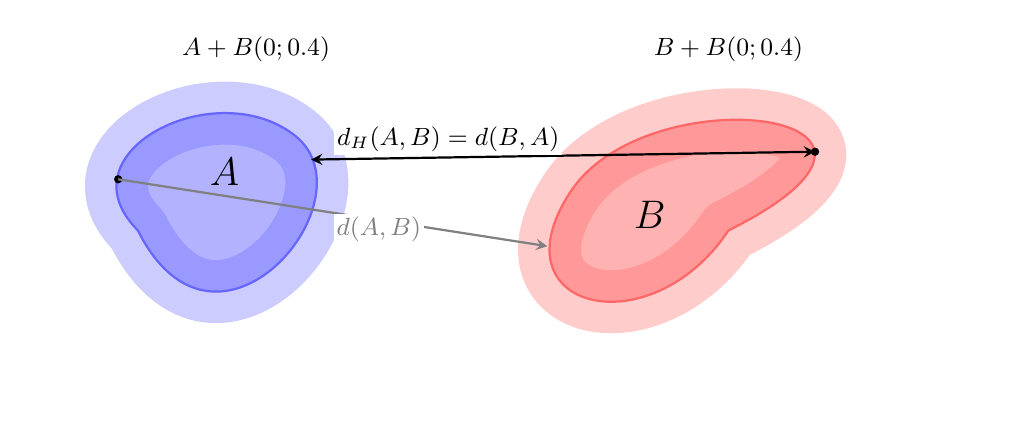
\begin{tikzpicture}[
    set/.style={draw, thick, fill opacity=0.5},
    dist/.style={-stealth, thick, gray},
    hausdorff_dist/.style={stealth-stealth, thick},
    label/.style={midway, fill=white, inner sep=1pt, font=\small}
]
    % Define the paths for the two sets
    \def\pathA{(-2,0) .. controls (-3,1) and (-1,2) .. (0,1.2) .. controls (1,0.4) and (-1,-2) .. (-2,0)}
    \def\pathB{(3.5,0.5) .. controls (2.5,-1) and (4.5,-1.5) .. (5.5,0) .. controls (8.5,1.5) and (4.5,2) .. (3.5,0.5)}

    % Epsilon radius for the halo
    \def\varepsilon{0.4}

    % Draw the halos (epsilon-neighborhoods) in the background
    \begin{scope}[on background layer]
        % Halo for A
        \draw[line width=2*\varepsilon cm, blue, opacity=0.2, line cap=round, line join=round] \pathA;
        \node[font=\small] at (-0.5, 2.3) {$A + B(0; \varepsilon)$};

        % Halo for B
        \draw[line width=2*\varepsilon cm, red, opacity=0.2, line cap=round, line join=round] \pathB;
        \node[font=\small] at (5.5, 2.3) {$B + B(0; \varepsilon)$};
    \end{scope}
    
    % Draw the actual sets on top
    \fill[blue!60, set] \pathA;
    \node at (-0.9, 0.75) {\Large $A$};

    \fill[red!60, set] \pathB;
    \node at (4.5, 0.2) {\Large $B$};
    
    % --- Illustrate the distances ---
    
    % The point on A furthest from B (approximate)
    \coordinate (a_furthest) at (-2.25, 0.65);
    \fill (a_furthest) circle (1.5pt) node[below left, font=\tiny] {};
    
    % The point on B that is closest to a_furthest
    \coordinate (b_closest_to_a) at (3.2, -0.2);
    
    % Draw the one-sided distance for a single point
    \draw[dist] (a_furthest) -- (b_closest_to_a) node[label, below right] {$d(A,B)$};

    % The point on B furthest from A (approximate)
    \coordinate (b_furthest) at (6.6, 1);
    \fill (b_furthest) circle (1.5pt);
    
    % The point on A closest to b_furthest
    \coordinate (a_closest_to_b) at (0.2, 0.9);
    
    % d(B,A) is larger, so it defines the Hausdorff distance.
    \draw[hausdorff_dist] (b_furthest) -- (a_closest_to_b) node[label, above left ] {$d_H(A,B) = d(B,A)$};
    
\end{tikzpicture}
\caption{It is the smallest radius $\varepsilon$ such that the $\varepsilon$-neighborhood of each set contains the original other set. This neighborhood is visualized as the semi-transparent `halo' around each set.}
\label{fig:hausdorff_corrected}
\end{figure}

\newpage

\subsection{Completeness Properties}
One may now begin to question: ``Is this induced metric space always complete?''. The answer to that is no.
\begin{ex}
Consider the metric space $(\mathbb{Q}, d_E)$. Consider $A_n:=\left [\sqrt{2} - \frac{1}{n}, \sqrt{2} + \frac{1}{n} \right ] \cap  \mathbb{Q}$ for $n \in \mathbb{N}^+$. Each $A_n$ is closed (since $\left [ \sqrt{2} - \frac{1}{n}, \sqrt{2} + \frac{1}{2}\right ]$ is closed in $(\mathbb{R}, d_E)$ and $(\mathbb{Q}, d_E)$ is a subspace of $(\mathbb{R}, d_E)$), bounded and nonempty so $A_n \in \mathcal{K}(\mathbb{Q})$ for all $n \in \mathbb{N}^+$.
\begin{center}
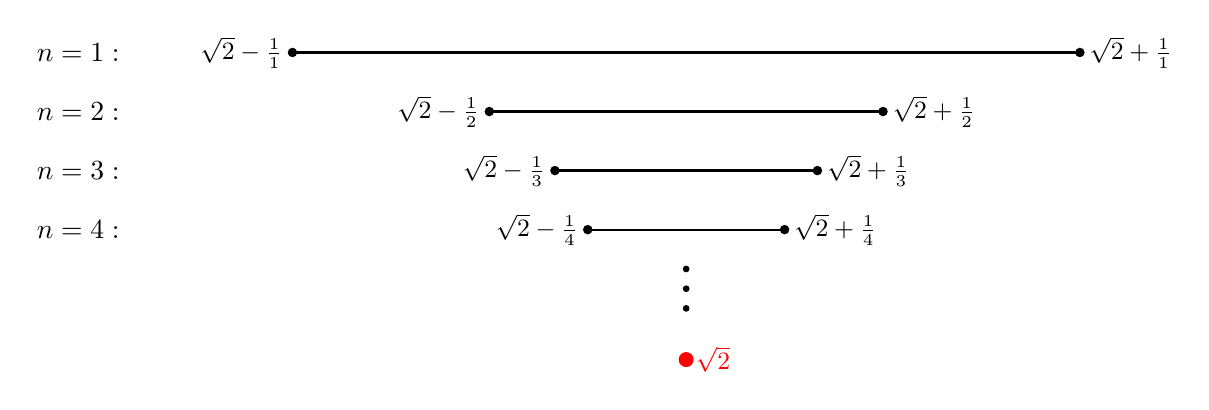
\begin{tikzpicture}[scale=5]
  
  % sqrt(2) ≈ 1.4142
  \def\srt{1.4142}
  
  % Draw 4 intervals
  \foreach \n in {1,2,3,4} {
    \pgfmathsetmacro\y{-(\n-1)*0.15}
    \pgfmathsetmacro\a{\srt - 1/(\n)}
    \pgfmathsetmacro\b{\srt + 1/(\n)}
    
    % Interval line
    \draw[thick] (\a,\y) -- (\b,\y);
    % Endpoints
    \filldraw[black] (\a,\y) circle (0.3pt) node[left] {\small$\sqrt{2} - \frac{1}{\n}$};
    \filldraw[black] (\b,\y) circle (0.3pt) node[right] {\small$\sqrt{2} + \frac{1}{\n}$};
    
    % Label on the left
    \node[left] at (0, \y) {$n=\n :$};
  }
  
  % Dots for continuation
  \foreach \i in {1,2,3} {
    \pgfmathsetmacro\y{-4*0.15 - \i*0.05 + 0.1}
    \draw[fill=black] (\srt,\y) circle (0.2pt);
  }

  % Final limiting point
  \pgfmathsetmacro\ylimit{-4*0.15 - 4*0.07 + 0.1}
  \filldraw[red] (\srt,\ylimit) circle (0.5pt) node[right] {\small$\sqrt{2}$};

\end{tikzpicture}
\end{center}
We have that $A_1 \supseteq A_2 \supseteq A_3 \supseteq ...$, so $d_H(A_n, A_m) = d(A_n, A_m)$ for $n \le m$. But 
\begin{center}
    $d(A_n, A_m) = \sup \limits _{x\in \left [\sqrt{2}-\frac{1}{n}, \sqrt{2}+\frac{1}{n} \right ] \cap \mathbb{Q}} \inf \limits _{y\in \left [\sqrt{2}-\frac{1}{m}, \sqrt{2}+\frac{1}{m} \right ] \cap \mathbb{Q}} |x-y| = \frac{1}{n} - \frac{1}{m} \to 0 \text{ as } m,n\to \infty$.    
\end{center}
 So $(A_n)$ is Cauchy. To show $A_n$ does not converge in $\mathcal{K}(\mathbb{Q})$, we show $A_n \to \{\sqrt{2}\} = S$ in $(\mathcal{K}(\mathbb{R}), d_H)$, induced from $(\mathbb{R}, d_E)$. We have that

\begin{center}
    $d_H (A_n, S) =$
    $
    \begin{cases}
        d(A_n, S) & \text{ if } d(A_n, S) \ge d(S, A_n) \\ d(S, A_n) & \text{ if } d(A_n, S) < d(S, A_n)
    \end{cases} \underbrace{\ \ \  = \ \ \ }_{\text{   Theorem~\ref{thm:d_properties}\textcolor{blue}{.4}  }} \begin{cases}
        d(a_n, \sqrt{2}) & \text{ if } d(A_n, S) \ge d(S, A_n) \\ d(\sqrt{2}, a_n) & \text{ if } d(A_n, S) < d(S, A_n)
    \end{cases} $ \\ ~\\ ~\\ $= d(a_n, \sqrt{2})
    $ for some $a_n \in A_n$
\end{center}
Clearly $a_n \to \sqrt{2}$, since $\sqrt{2} - \frac{1}{n} \le a_n \le \sqrt{2} + \frac{1}{n}$. So $d(a_n, \sqrt{2}) \to 0$ and so $d_H(A_n, S) \to 0$ as $n\to \infty$. But $S \notin \mathcal{K}(\mathbb{Q})$ so the sequence $(A_n)$ cannot converge in $(\mathcal{K}(\mathbb{Q}), d_H)$.
\end{ex}
~\\
This example powerfully demonstrates that the completeness of $(\mathcal{K}(X),d_H)$ is not guaranteed. It naturally leads to a crucial question: when is it complete? Is there a property of the underlying space $(X,d)$ that can guarantee that the space of its compact subsets is complete? The following theorem provides a definitive answer.

\begin{thm}
    Let $(X,d)$ be a complete metric space. Then the induced Hausdorff metric space $(\mathcal{K}(X), d_H)$ is complete.
\end{thm}
\begin{proof}
Let $(X_n)$ be a Cauchy sequence in $(\mathcal{K}(X), d_H)$. We will take a subsequence $X_{n_k}$ such that \[d_H(X_{n_{k+1}}, X_{n_k}) < 2^{-k}\]
We do it as such: 
\begin{itemize}
    \item For $\varepsilon = 2^{-1}, \ \  \exists N_1\in \mathbb{N}, \ \  \forall m,n\ge N_1: d_H(X_m, X_n) < 2^{-1}$. Let $n_1=N_1$. 
    \item We define $n_k \text{ for } k\ge 2$ recursively: 
    for $\varepsilon=2^{-k}, \ \  \exists N_k \in \mathbb{N}, \ \ \forall n,m\ge N_k: d_H(X_n, X_m ) <2^{-k} $. We then let $n_k = N_k + n_{k-1}+1$
\end{itemize}
Then, by definition, $n_{k+1}>n_k \ge N_k$ so $d_H(X_{n_{k+1}, }X_{n_k}) < 2^{-k}$. We now consider sequences $(x_n)$ such that $x_k \in X_{n_k}$ and $d(x_{k+1}, x_k)\le 2^{-k}$. We will say such a sequence satisfies property $(*)$. We first show such a sequence exists.

\begin{itemize}
    \item Let $x_1 \in X_{n_1}$. From $d_H(X_{n_{2}}, X_{n_1})<2^{-1}$, it follows that $d(x_1, X_{n_2}) \le d(X_{n_1}, X_{n_2}) < 2^{-1}$, so there is some $x_2 \in X_{n_2}$ such that $d(x_2, x_1) \le 2^{-1}$.

    \item For $k\ge 2$, we then recursively find $x_{k+1}\in X_{n_{k+1}}$, given $x_{k}\in X_{n_{k}}$, such that $d(x_{k+1}, x_{k}) \le 
    2^{-k}$ using that $d(x_k, X_{n_{k+1}}) \le d(X_{n_k}, X_{n_{k+1}}) < 2^{-k}$.
\end{itemize}
This sequence is Cauchy and thus converges in $(X,d)$. Let $Y = \left \{\lim \limits _{n \to \infty}x_n:(x_n) \text{ satisfies property } (*) \right \}$. We have to show that $Y$ is compact. To do so, we will show it is closed and totally bounded. Let $(y_n)$ be a sequence in $Y$ converging to some $y \in X$. Then, for each $n \in \mathbb{N}_0$, $y_n = \lim \limits _{m \to \infty } y_{nm}$ for some sequence $(y_{nm})_{m \in \mathbb{N}_0}$ satisfying $(*)$. We have that, for each $n \in \mathbb{N}_0$, $y_{n1} \in X_{n_1}$, so considering sequence $(y_{n1})_{n \in \mathbb{N}_0}$, there exists a subsequence $(n_k ^{(1)}) \subseteq \mathbb{N}_0$ such that $y_{{n_k^{(1)}}1} \to a_1$ for some $a_1 \in X_{n_1}$. Then, considering sequence $(y_{{n_k^{(1)}}2})$ in $X_{n_2}$, we get a further subsequence $y_{n_k^{(2)}2 } \to a_2 \in X_{n_2}$ where $n_k^{(2)} \subseteq n_k ^{(1)}$. Continuing this inductively, we get a subsequence $y_{{n_k}^{(r)}r} \to a_r \in X_{n_r} $ for each $r \in \mathbb{N}^+$. Then \[
d(a_{r+1}, a_r) = d \left (\lim \limits _{k \to \infty} y_{n_k ^{(r+1)}r+1}, \lim \limits _{k \to \infty} y_{n_k ^{(r)}r} \right ) 
\] 
But we have that $n_k ^{(r+1)} \subseteq n_k ^{(r)}$, so \[
 d \left (\lim \limits _{k \to \infty} y_{n_k ^{(r+1)}r+1}, \lim \limits _{k \to \infty} y_{n_k ^{(r)}r} \right ) = d \left (\lim \limits _{k \to \infty} y_{n_k ^{(r+1)}r+1}, \lim \limits _{k \to \infty} y_{n_k ^{(r+1)}r} \right ) = \lim \limits _{k \to \infty } d \left (\underbrace{y_{n_k ^{(r+1)}r+1}, y_{n_k ^{(r+1)}r}}_{\le 2^{-r}} \right ) \le 2^{-r}
\]
So sequence $(a_r)_{r \in \mathbb{N}^+}$ satisfies $(*)$. Finally, we show it converges to $y$. \[
d(a_r, y) = d \left (  \lim \limits _{k \to \infty } y_{n_k^{(r)}r}, y\right )
\]
For $k$ large enough, we get \[
d(a_r, y) = d \left (  \lim \limits _{k \to \infty } y_{n_k^{(k)}r}, y\right ) = \lim \limits _{k \to \infty }d \left ( y_{n_k^{(k)}r}, y\right ) = 0
\]
So $Y$ is closed. ~\\~\\
Let $\varepsilon > 0$. Choose $K$ large enough such that \[
\sum \limits _{i=K}^\infty 2^{-i} < \frac{\varepsilon}{2}
\]
If $y \in Y$, there is a sequence $(x_n)$ converging to $y$ satisfying $(*)$. But then \[
d(y,x _K) = \lim \limits _{n \to \infty} d(x_n, x_K) \le \lim \limits _{n \to \infty} \sum \limits _{i=K}^{n-1} d(x_{i+1}, x_i) \le \sum \limits _{i=K}^{\infty }d(x_{i+1}, i_n) \le \sum \limits _{i = K} ^\infty 2^{-i} < \frac{\varepsilon}{2}
\]
So $y \in B(x_K; \frac{\varepsilon}{2})$ with $x_K \in X_{n_K}$. So \[
Y \subseteq \bigcup \limits _{x_K \in X_{n_K}} B\left (x_{K}; \frac{\varepsilon}{2} \right )
\]
But $X_{n_K}$ is compact, so we can find a finite subcovering that also covers $Y$. That is, \[
Y \subseteq \bigcup \limits _{j=1}^{N} B \left (x_{K_j}, \frac{\varepsilon}{2} \right )
\]
So $Y$ is totally bounded and thus compact. We have shown $Y$ is nonempty and so $Y \in \mathcal{K}(X)$. We will show that $(X_{n_k}) $ converges to $Y$. \\ ~\\ Let $\varepsilon > 0$. Now $d_H(X_{n_k}, Y) = \max\{d(X_{n_k}, Y), d(Y, X_{n_k})\}$. 
\begin{enumerate}[label=(\arabic*)]
    \item First we consider $d(X_{n_k}, Y):$ \\ Take $K \in \mathbb{N}^+$ large enough such that \[\sum \limits_{n=K}^\infty 2^{-n}<\frac{\varepsilon}{2}\]
    Let $k \ge K $ so $n_k \ge K$. For any $x_{k} \in X_{n_k}$, by the construction above, create a sequence $(y_n)$ converging to some $y \in X$ with $y_k = x_k$. Then \[d(x_k, Y) \le d(x_k, y)=d(y_k, y) = d(y_k,\lim \limits _{p \to \infty}y_{k+p})=\lim \limits _{p \to \infty} d(y_k, y_{k+p}) \]  But \[d(y_k, y_{k+p})\le \sum \limits _{i=0}^{p-1} \underbrace{d(y_{k+i}, y_{k+i+1})}_{{< 2^{-(k+i)}}} <\sum \limits _{i=0}^{p-1} 2^{-(k+i)} = \sum \limits _{i=k}^{p+k-1}2^{-i } < \sum \limits _{i=K}^{\infty} 2^{-i} < \frac{\varepsilon}{2}\]So $\lim \limits _{p \to \infty} d(y_k, y_{k+p}) \le \frac{\varepsilon}{2} $ and thus $d(X_{n_k}, Y) < \varepsilon$.

    \item  Now we consider $d(Y, X_{n_k}):$ \\  Any $x\in Y$ has a sequence $(x_k)$ converging to it. Take $M$ large enough such that $k\ge M \implies d(x_k, x)< \frac{\varepsilon}{2}$. But $d(x, X_{n_k})\le d(x_k, x)<\frac{\varepsilon}{2}$ so $d(Y, X_{n_k}) \le \frac{\varepsilon}{2} < \varepsilon$
\end{enumerate}
So taking $N = M+K$, it follows that $k \ge N \implies d_H(X_{n_K}, Y)<\varepsilon$, so $X_{n_k} \to Y$, and since $(X_{n_k})$ is a convergent subsequence of a Cauchy sequence, it follows that $X_n \to Y$.
\end{proof}
~\\We can also show the converse is true
\begin{thm}
    If $(\mathcal{K}(X), d_H)$ is complete, then $(X, d)$ is complete 
\end{thm}

\begin{proof}
    Suppose that $(x_n)$ is Cauchy in $(X,d)$. Consider the sets $X_n := \{x_n\}$. These are compact. By Theorem~\ref{thm:d_properties}\textcolor{blue}{.4}, \[d_H(X_n, X_m) = d(x_n, x_m) \to 0 \text{ as } n\to \infty\]
    So $(X_n)$ is Cauchy in $(\mathcal{K}(X), d_H)$ and thus $X_n \to Y$ for some $Y\in \mathcal{K}(X)$. We claim that $|Y| = 1$. Assume, for a contradiction, that $Y$ contains at least two distinct points $a$ and $b$. Clearly then $d_H(X_n, Y)=d(Y,X_n)$. Let $r = d(a,b) >0$. There is some $N \in \mathbb{N}^+$ such that $d(Y, X_N)<\frac{r}{2}$. But \[d(Y, X_N) = \sup \limits _{y\in Y}d(y, X_N) = \sup \limits _{y\in Y}d(y, x_N)\]So $d(Y, X_N) < \frac{r}{2}$ implies $d(x_N, a) < \frac{r}{2}$ and $d(x_N, b) < \frac{r}{2}$. Then, by the triangle inequality, \[d(a,b) \le d(a, x_N) + d(x_N, b) <r\] which is a contradiction. So $Y = \{x\}$ for some $x \in X$, and $d_H(X_n, Y)=d(x_n, x)$ so $d(x_n, x) \to 0$ as $n \to \infty$, so $x_n \to x$ as $n \to \infty $ in $(X,d)$ meaning $(X,d)$ is complete.
\end{proof}

~\\These two theorems then imply
\begin{thm}\label{thm:haus_met}
    A metric space $(X,d)$ is complete if and only if the induced Hausdorff metric space $(\mathcal{K}(X), d_H)$ is complete
\end{thm}

\newpage

\subsection{Additional Properties}
We end this section by proving a theorem that will be useful later on.

\begin{thm}\label{thm:haus_additional}
    For $A_1, ..., A_N, B_1, ..., B_N \in \mathcal{K}(X)$, we have
    \begin{center}
        $d_H \left ( \bigcup \limits _{n=1}^N A_n, \bigcup \limits _{n=1}^N B_n \right ) \le \max \limits _{1\le n\le N} d_H(A_n, B_n)$
    \end{center}
\end{thm}

\begin{proof}
    First note that finite unions of compact sets are compact, and in this case, non-empty, so \[\bigcup \limits _{n=1}^N A_n, \bigcup \limits _{n=1}^N B_n \in \mathcal{K}(X)\]Now we will show that $d_H(A_1 \cup A_2, B_1 \cup B_2) \le \max\{d_H(A_1, B_1), d_H(A_2, B_2)\}$ and then the above result holds by induction. Without loss of generality, let $d_H(A_1 \cup A_2, B_1 \cup B_2) = d(A_1 \cup A_2, B_1 \cup B_2)$.
Consider $a \in A_1$. Clearly \[d(a, B_1\cup B_2) = \inf \limits _{b\in B_1\cup B_2} d(a,b) \le \inf \limits _{b\in B_1} d(a,b) = d(a,B_1).\] Similarly, for $a \in A_2$, $d(a, B_1 \cup B_2) \le d(a, B_2)$. Thus, for any $a\in A_1 \cup A_2$, \[d(a, B_1 \cup B_2)  \le \max \{d(A_1,B_1), d(A_2, B_2) \} \le \max \{d_H(A_1, B_1), d_H(A_2, B_2)\}\] So $d_H(A_1\cup A_2, B_1 \cup B_2) = d(A_1\cup A_2, B_1 \cup B_2)  \le \max \{d_H(A_1,B_1), d_H(A_2, B_2)\}$
\end{proof}
~\\
\noindent\fbox{%
    \begin{minipage}{\textwidth}
        \textbf{Historical Context:} The Hausdorff metric was introduced by Felix Hausdorff in 1914, originally motivated by questions in set theory and topology. Its applications now span from image processing to machine learning, where it measure similarity between shapes.
    \end{minipage}%
}
% ~\\~\\
% \noindent\fbox{%
%     \begin{minipage}{\textwidth}
%         \textbf{Key Takeaways:} \begin{enumerate}
%             \item The Hausdorff metric provides a rigorous way to measure distances between compact sets.
%             \item $(\mathcal{K}(X), d_H)$ is complete if and only if $(X,d)$ is complete.
%             \item The metric is well-suited for studying the convergence of geometric structures.
%             \item The metric is an essential tool for fractal geometry (which we will see later).
%         \end{enumerate}
%     \end{minipage}%
% }


\newpage

\section{Hausdorff Measures and Dimensions}
\subsection{Motivation}
The Hausdorff Measure provides a natural way to assign sizes to sets, much like the Lebesgue Measure. In fact, we will later see that the Hausdorff Measure differs from the Lebesgue Measure only by a multiplicative constant. This naturally raises the question: why introduce a new measure if the Lebesgue Measure already exists? There are several important reasons:
    \begin{itemize}
        \item \textbf{Limitations of the Lebesgue Measure.} While the Lebesgue measure works well for familiar sets such as intervals, squares, and cubes, it struggles with sets that have more complicated geometry. For such sets, especially those arising in fractal geometry, the Lebesgue measure is not well-suited. We therefore need a more flexible notion of size - one that can handle irregular structures and even assign them dimensions.

        \item \textbf{Lower-dimensional sets in $\mathbb{R}^n$.} The idea of dimension is that it determines which measure to use. For example, a line is 1-dimensional (length), a square is 2-dimensional (area), and a cube is 3-dimensional (volume). Now in $\mathbb{R}^n$, the Lebesgue measure $\lambda _n$ assigns meaninful values to sets of full dimension $n$. For a lower-dimensional set $A\subseteq\mathbb{R}^n$, we have $\lambda_n(A)=0$, but we cannot use $\lambda_{n-1}$ on $\mathbb{R}^n$ because $\lambda _{n-1}$ is not defined in $\mathbb{R}^n$. To illustrate this, take the following example:


                    \begin{center}

                    
%     \begin{tikzpicture}
% % Ejes coordenados
% \draw[->] (-1,0) -- (3,0) node[right] {$x$};
% \draw[->] (0,-1) -- (0,3) node[above] {$y$};

% % Curvas en el primer cuadrante
% \draw[smooth] (0.5,2) .. controls (1,2.2) and (1.5,2) .. (2,2);
% \draw[smooth] (1,1) .. controls (1.5,1.5) and (2,1.5) .. (2.5,1);
% \draw[smooth] (1.5,0.5) .. controls (2,0.5) and (2.5,0.5) .. (3,0.5);
% \end{tikzpicture}

\begin{tikzpicture}[scale=1]
  % Axes
  \draw[->] (-0.5,0) -- (4.5,0) node[right] {$x$};
  \draw[->] (0,-0.5) -- (0,5.2) node[above] {$y$};
  
  % Curve
  % \draw[thick,blue,domain=0.3:4,smooth,variable=\x]
  %   plot ({\x},{0.5 + atan(deg(\x)});
  \draw[thick, blue, domain = 0.3:2.1, smooth, variable = \x]
       plot ({\x},{1});

   \draw[thick, blue, domain = 2.1:4, smooth, variable = \x]
       plot ({\x},{0.5 + sqrt{\x}});

    \filldraw[white] (2.1,1.95) circle (1.5pt);
    \draw[line width=0.8pt] (2.1,1.95) circle (1.5pt);

\filldraw[black] (2.1,1) circle (1.5pt);
    \draw[line width=0.8pt] (2.1,1) circle (1.5pt);

    
  % Labels
  \node[blue] at (3,3) {$A$};
  \node at (2.2,-0.3) {A curve in $\mathbb{R}^2$};
\end{tikzpicture}


\end{center}


 Let $A$ be this curve. This curve has no area, so $\lambda_2(A)= 0$ (this curve has length so is 1-dimensional). On the other hand, $\lambda _1(A)$ is not defined. So, how can we measure this set? This is where we can use the Hausdorff measure.
    \item \textbf{Generality.} The Hausdorff measure applies to any metric space, whereas Lebesgue measure is tied specifically to Euclidean space $\mathbb{R}^n$ (i.e., the metric space $(\mathbb{R}^n, d_E)$)

    \item \textbf{Flexibility and structure.} The Hausdorff measure has useful properties - such as invariance under translations, and isometries, and scaling multiplies the measure value dependent on the dimension. While the Lebesgue measure does as well, the Hausdorff measure extends these properties to any metric space
    \item \textbf{Beyond integer dimensions.} Perhaps most importantly, the Hausdorff measure allows us to assign sizes and dimensions to sets even when their dimension is not an integer. This makes it the ideal tool for studying fractals and other objects with non-classical geometry.

    \end{itemize}

\newpage

\subsection{Intuitive Understanding}
Let $A \subseteq \mathbb{R}^n$ be a set. Our goal is to assign a notion of ``volume'' to $A$.  
A first attempt might be to take the diameter of $A$, denoted $\mathrm{diam}(A)$ (the largest distance between two points in $A$), and estimate the volume as $\mathrm{diam}(A)^n$. For example, in $\mathbb{R}^3$ this corresponds to placing a cube around $A$ with side length equal to $\mathrm{diam}(A)$ (see Figure 2).  
~\\~\\
Clearly, this estimate is far too basic. To refine it, we can cover $A$ by many smaller sets $\{E_i\}_{i \in \mathbb{N}^+} \subseteq \mathbb{R}^n$ and estimate its size by summing up the ``volumes'' of these sets. In Figure 3, for example, a sphere is covered by smaller sets, whose volume is estimated by cubes, and the total estimated volume is the sum of the volumes of all cubes in the covering.
~\\~\\
Formally, if $\{E_i\}_{i \in \mathbb{N}^+}$ is a covering of $A$, then
\[
\sum_{i=1}^\infty \bigl(\mathrm{diam}(E_i)\bigr)^n
\]
gives an estimate of the size of $A$.  
This estimate depends heavily on the particular covering chosen, and may include ``extra volume'' that is not part of $A$. To correct for this, we take the \emph{infimum} over all possible coverings of $A$.  
Moreover, we want the coverings to become finer and finer: as the diameters of the covering sets shrink, our approximation improves. In the limit, this process converges to the true volume of $A$. This explains how the Hausdorff construction captures the ``roughness'' or fine-scale detail of a set.
~\\~\\
The advantage of this approach is that it extends naturally beyond $\mathbb{R}^n$. In any metric space $(X,d)$, we use
\[
\mathrm{diam}(X) = \sup_{x,y \in X} d(x,y),
\]
and use coverings by sets of small diameter in the same way. This allows the Hausdorff measure to be applied in very general settings.

    \begin{center}

\begin{figure}[h]

    \begin{minipage}{0.4\textwidth}
    \label{fig:cube_sphere}
    \centering
        \includegraphics[scale = 0.45]{assets/cover_sphere_big_cube.png}
        
        \caption{A cube covering a sphere}
    \end{minipage}
    \begin{minipage}{0.1\textwidth}
    \centering
            $\Huge \Rightarrow$
    \end{minipage}
    \begin{minipage}{0.4\textwidth}
    \label{fig:cube_sphere_cover}
        \includegraphics[scale = 0.45]{assets/cover_sphere_small_cubes.png}
        \caption{A sphere estimated by smaller cubes}
    \end{minipage}
\end{figure}
    \end{center}

\newpage

\subsection{Hausdorff Measures}
\begin{defn}
    Let $(X, d)$ be a metric space with $\diam (\emptyset) :=0$. For $d \geq 0$, $\delta > 0$, and $\mathcal{H}^d_\delta :\mathcal{P}(X) \to \overline{\mathbb{R}}_{ +} $, define:
        \begin{align}
            \mathcal{H}_\delta^d(A) := \inf\left\{\sum \limits _{i =1}^\infty (\diam (E_n))^d : A \subseteq \bigcup \limits _{n=1}^\infty E_n \text { and} \diam(E_n) \le \delta \right\}
        \end{align}
        We say such a covering $\{E_n\}_{n\in \mathbb{N}^+}$ is a $\delta$-covering. If $A$ does not possess any $\delta$-coverings, we have $\mathcal{H}_\delta ^d(A) := \inf \emptyset =\infty $.
        \\ The Hausdorff $d$-measure is then a function $\mathcal{H}^d: \mathcal{P}(X) \to \overline{\mathbb{R}}_+$ defined by:
        \begin{align}
            \mathcal{H}^d(A) := \lim_{\ \delta \to 0^+} \mathcal{H}_\delta^d(A) = \sup_{\delta > 0} \mathcal{H}_\delta^d(A)
        \end{align}
         If $ d=0$: Define $\diam (\emptyset)^0=0$ and use the interpretation $0^0=1$ for any other sets, so that $\mathcal{H}^0$ is the counting measure (which we will prove). Note the following:
    
    \begin{itemize}
        \item All we require is $\diam (E_n) \le \delta $ for each $n \in \mathbb{N}^+$, so if $\delta \le \delta'$, then $ \mathcal{H}_\delta ^d(A) \ge \mathcal{H}_{\delta'}^d(A) $. The supremum form above in $(2)$ is thus valid
        \item An alternative definition allows us to normalise the Hausdorff measure: $\mathcal{H}^d(A) = c_d \cdot \lim \limits _{\ \delta \to 0^+} \mathcal{H}_\delta^d(A)$. In metric space $(\mathbb{R}^d, d_E)$, we will denote the normalized Hausdorff measure as $\mathcal{H}^d_N(A) :=\alpha (d) \mathcal{H}^d(A)$ for:
            \[
            \alpha (d) :=\frac{\pi ^{d/2}}{2^d \ \Gamma (d/2 + 1)}, \ \ \ \ \ \ \ \ \ \ \Gamma (t):= \int \limits _0 ^\infty e^{-x}x^{t-1}dx
            \]
        \item We can consider finite $\delta$-covers $\{E_n\}_{n=1}^N$ for $N\in \mathbb{N}^+$, by taking $E_m=\emptyset$ for $m\ge N+1$ and then $\sum \limits _{n=1}^N (\diam (E_n))^d = \sum \limits _{n=1}^\infty (\diam (E_n))^d$
    \end{itemize}
\end{defn}
\begin{thm}~\label{thm:ball_vol}
    To examine $\alpha (d)$, in $\mathbb{R}^d$, we prove that, for $r > 0$, $vol(B(\mathbf{0}; r)) = vol(B(\mathbf{0};1)) \cdot r^d$,
\end{thm}

\begin{proof}
    Using Tonelli's Theorem,
    \[vol (B(\mathbf{0};r)) = \int_{B(\mathbf{0};r)} 1d\lambda _d = \idotsint _{B(\mathbf{0};r)} 1dx_1dx_2...dx_d\]
    Our points $(x_1,...,x_d) \in B(\mathbf{0}; r)$ satisfy $x_1^2 + x_2^2 + \dots +x_d^2 \le r^2 \iff \left (\frac{x_1}{r} \right)^2 + \left (\frac{x_2}{r} \right)^2 + \dots + \left (\frac{x_d}{r} \right)^2 \le 1 $.
    Now, using the transformation $r\mathbf{y} = \mathbf{x}$ with jacobian matrix
    \[
    \mathbf{J} = \begin{bmatrix}
        r & 0 & 0 & ... & 0 \\
        0 & r & 0 & ... & 0 \\
         \vdots &  \vdots & \vdots & \ddots & \vdots \\ 
         0 & 0 & 0 & \dots & r
    \end{bmatrix}, \ \ \ |\mathbf{J}| = r^d
    \]
    Our integral becomes, using Tonelli's Theorem again,
    \begin{align*}
        \idotsint _{B(\mathbf{0};r)} 1dx_1dx_2...dx_d & = \idotsint _{B(\mathbf{0};1)} r^ddx_1dx_2...dx_d \\ & = r^d \lambda _d(B(\mathbf{0};1)) = r^d vol(B(\mathbf{0};1))
    \end{align*}
\end{proof}

\newpage 
\begin{thm}
    While the normalising constant $\alpha (n)$ may seem weird, it is in fact:
    \[
    \frac{\pi ^{n/2}}{2^n \  \Gamma (n/2 + 1)} = \frac{\lambda_n(B_n(\mathbf{0};1))}{2^n} \text{ when } n\in \mathbb{N}^+ \text{ and } B_n(0;1) \text{ is the unit ball in } \mathbb{R}^n
    \]    
    
\end{thm}

\begin{proof}
    % $\lambda_n(B) = \text{volume of } B$ and $B = \{(x_1, ..., x_n)\in \mathbb{R}^n:x_1^2+x_2^2+...+x_n^2=1\}$ so $\lambda_n(B) = \int \chi _B d\lambda _n$, which, by Tonelli's Theorem, we get $ \int \chi _B d\lambda _n = \int _\mathbb{R} \int _\mathbb{R} ...\int _\mathbb{R} \chi _B(x_1, ..., x_n) d\lambda (x_1) d\lambda (x_2)...d\lambda (x_n) $. We can write $B = \{(r, \theta _1,...,\theta _{n-1}):0\le r\le 1, 0\le \theta _i\le 2\pi \}$ in polar coordinate form, and so $\int _\mathbb{R} \int _\mathbb{R} ...\int _\mathbb{R} \chi _B(x_1, ..., x_n) d\lambda (x_1) d\lambda (x_2)...d\lambda (x_n) =\int \limits _{0}^1 \int \limits _0 ^{2 \pi } ... \int \limits _0 ^{2 \pi }$ 
    We will use a recursive approach. Let $\kappa_n = \lambda_n(B_n(\mathbf{0};1)) = vol(B_n(\mathbf{0};1))$. We will write points in $\mathbb{R}^n$ in the form $(x,y,\mathbf{z})$ where $\mathbf{z}\in \mathbb{R}^{n-2}$. Then, using Tonelli's Theorem, and that $\lambda _n = \lambda _{n-2} \otimes \lambda _2$
    \begin{align*}
        \lambda_n(B_n(\mathbf{0};1)) = \int _{B_n(\mathbf{0};1)} 1d \lambda _n & = \int_{B_2(\mathbf{0};1)} \int_{\{\mathbf{z} \in \mathbb{R}^{n-2}:||\mathbf{z}||_{n-2}^2 \le1-x^2-y^2 \}} 1d\lambda _{n-2}(\mathbf{z}) d\lambda _2(x,y) \\ & = \int_{B_2(\mathbf{0};1)} \int_{\{\mathbf{z} \in \mathbb{R}^{n-2}:||\mathbf{z}||_{n-2} \le \sqrt{1-x^2-y^2} \}} 1d\lambda _{n-2}(\mathbf{z}) d\lambda _2(x,y)
        \\ & = \int_{B_2(\mathbf{0};1)} \int_{B_{n-2}(\mathbf{0};\sqrt{1-x^2-y^2})} 1d\lambda _{n-2}(\mathbf{z}) d\lambda _2(x,y)
        \\ & = \int_{B_2(\mathbf{0};1)} \kappa _{n-2} \left(\sqrt{1-x^2-y^2} \right ) ^{n-2}d\lambda _2(x,y)
        \\ & = \kappa _{n-2}\iint _{B_2(\mathbf{0};1)} \left ( \sqrt{1-x^2-y^2} \right )^{n-2} dxdy
    \end{align*}
    Where the final step uses Tonelli's Theorem again. Using polar coordinates, we get:
    \begin{align*}
        \lambda _n(B_n(0;1)) &= \kappa _{n-2}\int _{0}^{2 \pi } \int _{0}^1 r\left (\sqrt{1-r^2} \right )^{n-2} drd\theta \\ & = \frac{2\pi }{n} \kappa _{n-2}
    \end{align*}
    So we have a recursive equation $\kappa_{n} = \frac{2\pi }{n} \kappa _{n-2}$ with $\kappa_1 = 2$, and $\kappa_2 = \pi r^2$. Then \[\kappa _n = \frac{\pi ^{n/2}}{\Gamma (\frac{n}{2}+1)}\] is the solution (using Theorem~\ref{thm:gamma} when simplifying)
    
\end{proof}

~\\Another question one may have is that in our definition of $\mathcal{H}_\delta ^d$, we only require $\diam (E_n) \le \delta$. So our smaller coverings that are more accurate are already accounted for here. Why can't we then use $\mathcal{H}^d_\delta$ as our measure value? Why must we take the limit as $\delta \to 0$? This next example shows that $\mathcal{H}^d_\delta $ is merely an under-approximation of the true value. We need the limit as $\delta \to 0^+$ to accurately describe the size. 

\begin{ex}
~\\
        \begin{figure}[htbp]
    \centering
    \begin{minipage}{0.6\textwidth}

        Take the square $[0,1] \times [0,1]$. This is 2-dimensional, so we expect the 1-dimensional measure of this set to be $\infty$ (with the 1-dimensional measure measuring length, not area). We prove this fact more rigorously in the example below. But we can cover the square with itself, and the diameter of the square is $\sqrt{2}$ so if we considered $\delta \ge \sqrt{2}$, then $\mathcal{H}^1_{\delta} ([0,1] \times [0,1]) \le \sqrt{2}$. So sending $\delta \to 0^+$ is thus important.
        ~\\~\\~\\ ~\\
    \end{minipage}
    \hfill
    \begin{minipage}{0.35\textwidth}
        \centering
        \includegraphics[scale=0.3]{assets/square_inf_measure.png}
        \caption{$\mathcal{H}^1([0,1] \times [0,1])$ visualized}
        \label{fig:square_measure}
    \end{minipage}
\end{figure}
            

    
\end{ex}


\newpage
~\\ Before looking at some examples of finding values with the Hausdorff measure, we first show that these are valid functions and $\mathcal{H}^d$ is a measure on an appropriate $\sigma$-algebra:
\begin{lem}

    For $d\ge 0$ and $\delta >0$, the functions $\mathcal{H}^d$ and $\mathcal{H}^d_\delta$ are well-defined. That is, $(1) \ \mathcal{H}^d_\delta $ exists for any set, $(2) \ \mathcal{H}^d $ exists for any set, $(3) \ \mathcal{H}^d_\delta\ge 0$ and $(4) \ \mathcal{H}^d \ge 0$
\end{lem}

\begin{proof} Let $A \in \mathcal{P}(X)$
    \begin{enumerate}[label=(\arabic*)]
    \item If $A$ has a $\delta$-covering $\{E_n\}_{n\in \mathbb{N}^+}$, then $\diam (E_n) \ge 0$ implies $\sum \limits _{n=1}^\infty (\diam (E_n))^d \ge 0$. So $0$ is a lower bound for $\left\{\sum \limits _{i =1}^\infty (\diam (E_i))^d : A \subseteq \bigcup \limits _{i=1}^\infty E_i \text { and} \diam(E_i) \le \delta \right\}$ and, by The Completeness Axiom, the infimum exists. If $A$ has no $\delta$-covering, then $\mathcal{H}^d_\delta(A)=\infty$
    \item If there is $\delta >0$ such that $\mathcal{H}^d_\delta (A) = \infty$, then $\mathcal{H}^d(A) = \infty$. Otherwise, we consider $\left \{\mathcal{H}^d_\delta (A):\delta >0 \right \}$. If this set is bounded by a real number, by the Completeness Axiom, the supremum exists. If it is not, then the supremum is $\infty$. In all cases, $\mathcal{H}^d$ exists.
    
    \item From $(1)$, if $A$ has no $\delta$-covering, then $\mathcal{H}^d_\delta(A)=\infty \ge 0$. If $A$ has a $\delta$-covering, then $0$ is a lower bound and thus $\mathcal{H}^d_\delta (A)\ge 0$
        \item This follows from $\mathcal{H}^d(A) \ge \mathcal{H}^d_\delta(A)\ge 0$
    \end{enumerate}
\end{proof}
~\\Right now, $\mathcal{H}^d$ is not a measure. We will show $\mathcal{H}^d$ is an outer measure, which will allow us to use Caratheodory's Extension Theorem to restrict the domain and make it a measure.

\begin{thm}
    Let $0\le d<\infty$ and $\delta >0$. Then the Hausdorff $d$-measure $\mathcal{H}^d:\mathcal{P}(X) \to \overline{\mathbb{R}}_+$ and $\mathcal{H}^d_\delta :\mathcal{P}(X) \to \overline{\mathbb{R}}_+$ are outer measures
\end{thm}

\begin{proof} $ $
    \begin{enumerate}
        \item \textbf{Empty Set:} By definition, by covering $\emptyset$ with itself, $\mathcal{H}^0_\delta (\emptyset) \le (\diam \emptyset)^0=0$. So $\mathcal{H}^0_\delta (\emptyset)=0$ and $\mathcal{H}^0(\emptyset)=0$.
        
         If $d \ne 0$, $\diam (\emptyset)=0 \implies \mathcal{H}^d_\delta(\emptyset)=0$, by again covering $\emptyset $ with itself and thus $\mathcal{H}^d(\emptyset)=0$.
        \item \textbf{Monotonicity:} Let $A \subseteq B$. It follows that if $\{E_n\}_{n\in \mathbb{N}^+}$ is a $\delta$-covering for $B$, then it is also a $\delta$-covering for $A$. Thus we have $\mathcal{H}_\delta ^d(A) \le \mathcal{H}_\delta ^d(B) \implies \mathcal{H} ^d(A) \le \mathcal{H} ^d(B)$. If $A$ has no $\delta$-coverings, then neither does $B$ and so $\mathcal{H}^d_\delta  (A)=\mathcal{H}^d _\delta (B)=\infty$, meaning $\mathcal{H}^d(A) \ge \mathcal{H}^d_\delta (A)=\infty$ and $\mathcal{H}^d(B)\ge \mathcal{H}^d_\delta (B)=\infty$. If $B$ has no $\delta$-coverings, then it is trivial that $\mathcal{H} ^d_\delta (A)\le \mathcal{H}^d(A)\le \mathcal{H}^d_\delta (B) = \mathcal{H}^d(B)=\infty$.
        
        \item \textbf{$\sigma$-subadditivity:} Let $\{\mathcal{A}_n\}_{n\in \mathbb{N}^+}$ be a sequence of subsets of $\mathcal{P}(X)$. We want that $\mathcal{H}^d _\delta \bigg(\bigcup \limits _{n=1}^\infty \mathcal{A}_n\bigg) \le \sum \limits _{n=1} ^\infty \mathcal{H}^d_\delta (\mathcal{A}_n)$. 
        If there exists some $n \in \mathbb{N}^+$ such that $\mathcal{A}_n$ has no $\delta$-coverings, then $\bigcup \limits _{n=1}^{\infty} \mathcal{A}_n$ has no $\delta$-coverings, and $\mathcal{H}^d _\delta \bigg(\bigcup \limits _{n=1}^\infty\mathcal{A}_n\bigg) = \sum \limits _{n=1} ^\infty \mathcal{H}^d_\delta (\mathcal{A}_n)= \infty$. So assume that every $\mathcal{A}_n$ has a $\delta$-covering and
        let $\varepsilon>0$. For each $n\in \mathbb{N}^+$, let $\{E_{nm}\}_{m\in \mathbb{N}^+}$ be a $\delta$-covering for $\mathcal{A}_n$ such that $\sum \limits _{m =1}^\infty\diam (E_{nm})^d <\mathcal{H}_{\delta} ^d(\mathcal{A}_n) + 2^{-n}\varepsilon$. Then 
        \[\bigcup \limits _{n=1}^\infty \mathcal{A}_n = \bigcup \limits _{n=1} ^ \infty \bigcup \limits _{m=1}^\infty E_{nm} = \bigcup \limits _{(n,m) \in \mathbb{N}^+ \times \mathbb{N}^+}E_{nm} \]So $\{E_{n,m}\}_{n,m \in \mathbb{N}^+ \times \mathbb{N}^+}$ is a $\delta$-covering for $\bigcup \limits _{n=1}^{\infty} \mathcal{A}_n$, and thus
          \[\mathcal{H}_\delta ^d\bigg(\bigcup \limits _{n=1}^\infty \mathcal{A}_n\bigg) \le \underbrace{\sum \limits _{n,m \in \mathbb{N}^+} \diam (E_{nm})^d = \sum \limits _{n=1}^\infty \sum \limits _{m =1}^\infty  \diam (E_{nm})^d}_{\diam (E_{nm}) \ge 0 \text{ so we use Tonelli's theorem for sums (\ref{thm:tonelli-sums})}} <\sum \limits _{n=1} ^\infty (\mathcal{H}_{\delta }^d(\mathcal{A}_n)+2^{-n}\varepsilon )=\sum \limits _{n=1}^\infty \mathcal{H}_\delta ^d(\mathcal{A}_n)+\varepsilon\] 
        This is true for all $\varepsilon>0$, so \[
        \mathcal{H}_\delta ^d\bigg(\bigcup \limits _{n=1}^\infty \mathcal{A}_n\bigg)  \le \sum \limits _{n=1}^\infty \mathcal{H}_\delta ^d(\mathcal{A}_n)
        \]
        and finally, taking the supremum,  \[\mathcal{H}^d \bigg(\bigcup \limits _{n=1}^\infty \mathcal{A}_n\bigg)\le \underbrace{\sup \limits _{\delta >0}\sum \limits _{n=1}^\infty \mathcal{H}^d _\delta(\mathcal{A}_n) \le \sum \limits _{n=1}^\infty \sup \limits _{\delta >0} \mathcal{H}_\delta ^d(\mathcal{A}_n)}_{\text{Subadditivity of Supremum: Theorem \ref{thm:sub}}} = \sum \limits _{n=1}^\infty \mathcal{H}^d(\mathcal{A}_n)\]
    \end{enumerate}
    Thus both $\mathcal{H}^d$ and $\mathcal{H}^d_\delta$ are outer measures.
\end{proof}

\begin{thm}
    The restricted Hausdorff $d$-measure $\mathcal{H}^d |_{\mathcal{M}(\mathcal{H}^d)}$ is a complete measure on $\mathcal{M}(\mathcal{H}^d)$
\end{thm}

\begin{proof}
    This follows from Caratheodory's Extension Theorem, see Theorem~\ref{thm:caratheodory}
\end{proof}

% \begin{itemize}
%     \item While we only consider sets $A \in \mathcal{M}(\mathcal{H}^d)$, the coverings $\{E_n\}_{n\in \mathbb{N{}}}$ are any sets $E_n \subseteq X$. So each $E_n$ need not be measurable
%     \item But in fact, we can only consider nice sets, such as open/closed balls, cubes or Borel sets. Considering these sets, the infimum will be the same
%     \item A proof showing that we can only consider open balls is below
% \end{itemize}

% \begin{proof}
%     Let $\mathcal{BH}^d_\delta $ be the open ball Hausdorff measure. Clearly $\mathcal{H}^d_\delta \le \mathcal{BH}^d_\delta $, since every open ball $\delta$-covering is a $\delta$-covering. 
%     Let $A \in \mathcal{M}(\mathcal{H}^d)$ and $\{E_n\}_{n\in \mathbb{N}}$ be a $\delta$-covering for $A$. For each $n\in \mathbb{N}$, choose open ball $B_n \supseteq E_n$ with $\diam (B_n) \le \diam (E_n)+\varepsilon ^22^{-n}$. Then 
%     \[
%     \sum \limits _{n=1}^\infty (\diam(B_n))^d \le \sum \limits _{n=1}^\infty (\diam (E_n) + \varepsilon^2 2^{-n})^d \le \sum \limits _{n=1}^\infty \diam (E_n)^d + \varepsilon
%     \]
%     for $\varepsilon$ small enough. Thus we get $ \mathcal{BH}^d_\delta \le \mathcal{H}^d_\delta $ and so $\mathcal{BH}^d_\delta =\mathcal{H}^d_\delta $
% \end{proof}

% \begin{lem}
%     $\mathcal{M}(\mathcal{H}^d)  \ne \mathcal{P}(X)$. This will be obvious once we show $\mathcal{H}^1 = \lambda_1$ for metric space $(\mathbb{R}, d_E)$. Then we consider the Vitali set. While $\mathcal{H}^1(\mathcal{V})$ exists for the Vitali set, $\mathcal{V}$ does not satisfy Caratheodory's Criterion (proof via lebesgue contradiction, the idea is that if we force the Vitali set $\mathcal{V}$ to be measurable, and consider $\mathcal{H}^1$ on $\sigma (\mathcal{M}(\mathcal{H}^d) \cup \{\mathcal{V} \})$, then it is no longer a measure.)
% \end{lem}

% Note that the Vitali set, while not measurable, the Hausdorff $1$-measure is defined. 

~\\ For now, assume all Lebesgue measurable sets are Hausdorff measurable. When we prove that $\mathcal{H}^n_N = \lambda _n$, then this will follow. Before we show $\mathcal{H}^1([0,1]\times [0,1])=\infty$, we will show a more general result, in that $\mathcal{H}^1((a,b]) = b-a$. For this, we need the lemma:

\begin{lem}
    For a measurable set $A \subseteq \mathbb{R}$, we have that $\lambda_1 (A) \le \diam (A)$
\end{lem}

\begin{proof}
    The case when $\diam (A)=\infty$ is trivial. If $\diam (A) < \infty$, then $A$ 
 is bounded, so both $\inf A \text{ and} \sup A$ exist and are finite, and $A \subseteq \left[\inf \limits A, \sup \limits A \right]$ and so $\lambda_1 (A) \le \lambda_1 \left(\left[\inf \limits A, \sup A\right]\right) = \sup \limits A - \inf \limits A = \diam (A)$
\end{proof}

\begin{ex}
We will show that $\mathcal{H}^1([a,b]) = b-a$: \\
Let $\delta >0$. We can divide $(a,b]$ into $m=\lceil \frac{b-a}{\delta} \rceil \le \frac{b-a}{\delta }+1 $ intervals with \[(a,b] = \bigg (\bigcup \limits _{n=1}^{m-1}(a+(n-1)\delta , a+n\delta ] \bigg) \cup (a+(m-1)\delta, b]\]Labeling each interval as $E_n$, each interval satisfies $\diam (E_n) \le \delta $, and so $\mathcal{H}_\delta ^1((a,b]) \le  m\delta \le (b-a)+\delta$. Sending $\delta \to 0^+$ yields $\mathcal{H}^1((a,b])\le b-a$ \\




\begin{figure}[htbp]
\centering
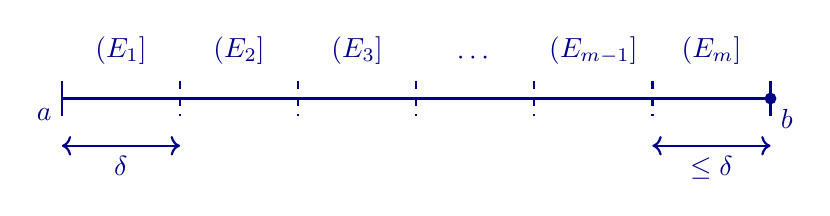
\begin{tikzpicture}[scale=1.5]
    % Color and styles
    \definecolor{myblue}{RGB}{0, 0, 139} % dark blue
    \tikzstyle{every path}=[myblue, thick]

    % Main interval [a,b]
    \draw[myblue] (0,0) -- (6,0);
    
    % Open bracket at a, closed at b
    \draw[myblue, thick] (0,0.15) -- (0,-0.15); % open bracket at a
    \node[below left] at (0,0) {$a$};
    
    \draw[myblue, thick] (6,0.15) -- (6,-0.15); % closed bracket at b
    \filldraw[myblue] (6,0) circle (0.04);
    \node[below right] at (6,0) {$b$};

    % Subdivision points
    \foreach \x in {1,2,3,4,5}
    {
        \draw[myblue,dashed] (\x,0.15) -- (\x,-0.15);
    }

    % Subinterval labels and brackets
    \node[above] at (0.5,0.2) {$\left( E_1 \right]$};
    \node[above] at (1.5,0.2) {$\left( E_2 \right]$};
    \node[above] at (2.5,0.2) {$\left( E_3 \right]$};
    \node[above] at (3.5,0.2) {$\cdots$};
    \node[above] at (4.5,0.2) {$\left( E_{m-1} \right]$};
    \node[above] at (5.5,0.2) {$\left( E_m \right]$};

    % Delta arrows
    \draw[myblue,<->] (0,-0.4) -- (1,-0.4) node[midway,below] {$\delta$};
    \draw[myblue,<->] (5,-0.4) -- (6,-0.4) node[midway,below] {$\leq \delta$};

\end{tikzpicture}
\end{figure}
~\\On the other hand, let $\{A_n\}_{n\in \mathbb{N}^+}$ be a $\delta$-covering for $(a,b]$. By defining $E_n :=A_n \setminus \bigcup \limits _{i=1}^{n-1} A_{i}$ for $n > 1$, and $E_1 = A_1$, we get the family $\{E_n\}_{n\in \mathbb{N}^+}$ is pairwise disjoint. Then $(a,b]=\bigcup \limits _{n=1}^\infty((a,b] \cap E_n) \implies \lambda_1 ((a,b]) =\sum \limits _{n=1}^\infty \lambda_1 ((a,b] \cap E_n)$, so $\sum \limits _{n=1}^\infty \lambda_1 ((a,b]\cap E_n)=b-a$ and $\sum \limits _{n=1}^ {\infty} \lambda_1 (E_n) \ge b-a$. But then \[\sum \limits _{n=1}^\infty \diam (A_n) \ge\sum \limits _{n=1}^\infty \diam (E_n) \ge \sum \limits _{n=1}^{\infty} \lambda _1(E_n) \ge b-a\]So $\mathcal{H}^1((a,b])=b-a$. 
\end{ex}

\begin{ex}
    Since $\mathcal{H}^1(\{a\}) = 0$ (by covering $\{a\}$ with itself), we get $\mathcal{H}^1([a,b]) = \mathcal{H}^1(\{a\}) + \mathcal{H}^1((a,b])=b-a$. Now  $\mathcal{H}^1(\{r\} \times [0,1]) = \mathcal{H}^1([0,1]) = 1$ (as simply viewing the segment $[0,1]$ as having $y$-coordinate $r$ in $\mathbb{R}^2$). So \[
    \mathcal{H}^1([0,1]\times [0,1]) \ge \mathcal{H}^1\left (\bigcup \limits _{n\in \mathbb{N}^+} \left \{ \frac{1}{n} \right\} \times [0,1] \right) = \sum \limits _{n\in \mathbb{N}^+} \mathcal{H}^1\left ( \left \{ \frac{1}{n} \right\} \times [0,1] \right) = \sum \limits _{n\in \mathbb{N}^+} 1=\infty\]
\end{ex}

~\\Now we can prove some simple properties about this measure: 

\begin{thm}\label{thm:measure_iso}
    For any $A \subseteq X$ (need not be measurable), $d \ge 0$, and an isometry $f: X \to X$, the Hausdorff measure is invariant under isometries. That is, \[
    \mathcal{H}^d(f(A)) = \mathcal{H}^d(A)
    \]
\end{thm}

\begin{proof}
First notice that for any $ B \subseteq X$, we have that \begin{align*}
\operatorname{diam}(f(B)) 
  &= \sup_{x,y \in f(B)} d(x,y) \\
  &= \sup_{x',y' \in B} d\!\left(f(x'), f(y')\right) \\
  &= \sup_{x',y' \in B} d(x',y') \\
  &= \operatorname{diam}(B).
\end{align*}

and 
\begin{align*}
\operatorname{diam}\!\big(f^{-1}(B)\big) 
  &= \sup_{x,y \in f^{-1}(B)} d(x,y) \\[6pt]
  &= \sup_{x,y \in f^{-1}(B)} d\big(f(x), f(y)\big) \\[6pt]
  &\leq \sup_{x',y' \in B} d(x',y') \\[6pt]
  &= \operatorname{diam}(B).
\end{align*}
So isometries reduce diameter (with respect to both the image and preimage).
Let $\delta >0$. Now if $A$ has a cover $\{E_n\}_{n\in \mathbb{N}^+}$, then \[
A \subseteq \bigcup \limits _{n\in \mathbb{N}^+} E_n \implies f(A) \subseteq f \left ( \bigcup \limits _{n\in \mathbb{N}^+} E_n\right ) = \bigcup \limits _{n \in \mathbb{N}^+} f(E_n)
\]
On the other hand, if $f(A)$ has a cover $\{F_n\}_{n\in \mathbb{N}^+}$, then \[
A \subseteq f^{-1}(f(A)) \subseteq f^{-1} \left ( \bigcup \limits _{n=1}^{\infty} F_n\right ) = \bigcup \limits _{n=1}^{\infty} f^{-1}(F_n)
\]
Let $\delta > 0$. Then $A$ has a $\delta$-cover if and only if $f(A)$ has a $\delta$-cover. If $A$ or $f(A)$ have no $\delta$-covers, $\mathcal{H}^d(f(A)) = \mathcal{H}^d(A) = \infty$. Assume that both $A$ and $f(A)$ have $\delta$-covers and let $\varepsilon > 0$, and $\{E_n\}_{n\in \mathbb{N}^+}$ be a $\delta$-cover for $A$. Then, by the above calculations, \[
\mathcal{H}^d_\delta (f(A)) \le \sum \limits _{n=1}^{\infty} \diam (f(E_n))^d = \sum \limits _{n=1}^{\infty} \diam (E_n)^d
\]
So $\mathcal{H}_\delta^d(f(A)) \le \mathcal{H}^d(A)$ which implies $\mathcal{H}^d(f(A)) \le \mathcal{H}^d(A)$. Now let $\{F_n\}_{n\in \mathbb{N}^+}$ be a $\delta$-cover for $f(A)$. Then \[
\mathcal{H}^d_\delta (A) \le \sum \limits _{n=1}^{\infty} \diam (f^{-1}(F_n))^d \le \sum \limits _{n=1}^{\infty} \diam (F_n)^d 
\]
So $\mathcal{H}^d_\delta(A) \le \mathcal{H}^d(f(A))$ meaning $\mathcal{H}^d(A) \le \mathcal{H}^d(f(A))$ and we can conclude $ \mathcal{H}^d(A)  =\mathcal{H}^d(f(A))$
\end{proof}
~\\
Applying this to the standard real metric
\begin{thm}
    Consider the Hausdorff measure in metric space $(\mathbb{R}^n, d_E) $ and take $A  \subseteq \mathbb{R}^n, \mathbf{a}\in \mathbb{R}^n, 0<t<\infty$. Define $A+\mathbf{a}:=\{\mathbf{x}+\mathbf{a}:\mathbf{x}\in A\}$ and $tA := \{t\mathbf{x}:\mathbf{x}\in A\}$. Then the Hausdorff measure is
    \begin{enumerate}[label = (\arabic*)]
        \item Invariant under translation: $\mathcal{H}^d(A+\mathbf{a})=\mathcal{H}^d(A)$
        \item Homogeneous of degree $d$: $ \mathcal{H}^d(tA)=t^d\mathcal{H}^d(A)$
    \end{enumerate}
\end{thm}
\begin{proof}
    Let $\delta > 0$. 
    \begin{enumerate}[label = (\arabic*)]
        \item Define $f: \mathbb{R}^n \to \mathbb{R}^n$ by $f(\mathbf{x}) = \mathbf{x} + \mathbf{a}$. Then \[
        |f(\mathbf{x}) - f(\mathbf{y})| = |\mathbf{x} + \mathbf{a} - \mathbf{y} - \mathbf{a}| = |\mathbf{x} - \mathbf{y}|
        \]
        So $f$ is an isometry and, by Theorem~\ref{thm:measure_iso}, $\mathcal{H}^d(A) = \mathcal{H}^d(f(A)) = \mathcal{H}^d(A + \mathbf{a})$

      
      \item Notice that $\{E_n\}_{n\in \mathbb{N}^+}$ is a $\delta$-covering for $tA$ if and only if $\left \{ \displaystyle \frac{E_n}{t}\right\}_{n\in \mathbb{N}^+}$ is a $\displaystyle \frac{\delta}{t}$-covering for $A$, and for any set $E \subseteq \mathbb{R}^n$, $\diam (tE)=t\diam (E)$. So
      \begin{align*}
          \mathcal{H}^d_\delta(tA) & = \inf \bigg \{\sum \limits _{n =1}^\infty \diam (E_n)^d : tA \subseteq \bigcup \limits _{n=1}^\infty E_n \text { and}  \diam(E_n) \le \delta \bigg \} 
          \\ &= \inf \bigg \{\sum \limits _{n =1}^\infty \diam \left (\frac{E_n}{t} \cdot t \right)^d : A \subseteq \bigcup \limits _{n=1}^\infty \frac{E_n}{t} \text { and}  \diam \left(\frac{E_n}{t}\right) \le \frac{\delta}{t} \bigg \}
          \\ &= \inf \bigg \{\sum \limits _{n =1}^\infty t^d\diam \left (\frac{E_n}{t} \right)^d : A \subseteq \bigcup \limits _{n=1}^\infty \frac{E_n}{t} \text { and}  \diam \left(\frac{E_n}{t}\right) \le \frac{\delta}{t} \bigg \}
          \\ &= t^d \inf \bigg \{\sum \limits _{n =1}^\infty \diam \left (\frac{E_n}{t} \right)^d : A \subseteq \bigcup \limits _{n=1}^\infty \frac{E_n}{t} \text { and}  \diam \left(\frac{E_n}{t}\right) \le \frac{\delta}{t} \bigg \}
          \\ &= t^d\mathcal{H}_{\delta / t} ^d(A)
      \end{align*}
        Then taking $\delta \to 0^+$ gives us that $\mathcal{H}^d(tA) = t^d\mathcal{H}^d(A)$
    \end{enumerate}
\end{proof}

% \begin{thm}
%     Let $A \in \mathcal{M}(\mathcal{H}^d)$ and $\delta>0$. Then the following conditions are equivalent:
%     \begin{enumerate}
%         \item $\mathcal{H}^d(A)=0$
%         \item $\mathcal{H}_{\delta}^d(A)=0$
%         \item $\forall \varepsilon>0, \exists \{E_n\}_{n\in \mathbb{N}}$ in $X$ such that $A \subseteq \bigcup \limits _{n=1}^\infty E_n$ and $\sum \limits _{n=1}^\infty \diam(E_n)^d < \varepsilon$
%     \end{enumerate}
% \end{thm}

% \begin{proof}
%     We will show $(1) \implies (2) \implies (3) \implies (1)$:
%     \begin{enumerate}[label=(\arabic*)]
%   \item 
%       $\implies \ $ (2): \\ $0\le \mathcal{H}_\delta ^d(A)\le \mathcal{H}^d(A)=0$ implies $\mathcal{H}^d_\delta (A)=0$
  
%   \item 
%       $\implies$ (3):\\
%   Let $\varepsilon>0$. Then $\mathcal{H}^d_{\delta}(A)=0$ means there is a $\delta$-covering $\{E_n\}_{n\in \mathbb{N}} $ of $A$ with $\sum \limits _{n=1}^\infty \diam (E_n)^d < \varepsilon$
%   \item 
%       $\implies$ (1):\\ 
%   Take $\Delta>0$, $\varepsilon >0$ and $\alpha = \min \{\Delta^d, \varepsilon\}$. By $(3)$, let $\{E_n\}_{n\in \mathbb{N}}$ be a covering with $\sum \limits _{n=1}^\infty \diam (E_n)^d < \alpha \le \varepsilon$. Then $\diam (E_n)^d < \alpha \le \Delta ^d \implies \diam (E_n)<\Delta $ and so $\mathcal{H}^d_\Delta (A) < \varepsilon$. Now $\mathcal{H}^d(A) = \sup \limits _{\Delta >0} \mathcal{H}^d_\Delta (A)  \le \varepsilon$. This is true for arbitrary $\varepsilon>0$ and thus $\mathcal{H}^d(A) = 0$
% \end{enumerate}
% \end{proof}

\noindent\fbox{%
    \begin{minipage}{\textwidth}
    \textit{The Hausdorff measure was introduced as a generalization of Lebesgue measure in order to provide a natural way of measuring sets with non-integer dimension, such as fractals. 
However, before exploring such applications, we must understand how the Hausdorff measure relates back to the classical Lebesgue measure. 
In fact, for integer dimensions, the Hausdorff measure recovers the Lebesgue measure, so it is a genuine extension of the Lebesgue measure.
It also highlights the flexibility of the Hausdorff measure. It is powerful enough to handle highly irregular sets while still coinciding with the classical values in the regular, Euclidean setting. }
    \end{minipage}%
}


\begin{thm}\label{thm:lebesgue_haus}
    We can relate the Hausdorff measure to the Lebesgue measure: 
    \begin{enumerate}
        \item $\mathcal{H}^0$ is the counting measure on measure space $(\mathbb{R}^n, \mathcal{P}(\mathbb{R}^n))$ (not just for $\mathcal{M}(\mathcal{H}^0)$)
        \item $\mathcal{H}^1_N=\mathcal{H}^1 = \lambda_1$ on $\mathbb{R}$ (as outer measures)
        \item $\mathcal{H}^n_N = \lambda_n$ on $\mathbb{R}^n$ for $n \in \mathbb{N}$ (as outer measures)
    \end{enumerate}
\end{thm}
\begin{proof}
    See Appendix B
\end{proof}~\\
\noindent Recall our intuitive understanding of dimension: 
\begin{itemize}
    \item Points are regarded as zero-dimensional,
    \item Lines (measured by length) are one-dimensional,
    \item Squares (measured by area) are two-dimensional,
    \item Cubes (measured by volume) are three-dimensional.
\end{itemize}
Hausdorff measures provide a rigorous way to capture these notions, extending the familiar ideas of length, area, and volume to more general sets. 
A key property of Hausdorff measures is that they are sensitive to the ``correct'' dimension of a set: when measured in a dimension that is too high, the measure vanishes; when measured in a dimension that is too low, the measure is infinite. 
The following theorem states this:

\begin{thm}\label{thm:why_dimension} For $0 \le s<t<\infty$ and $A \subseteq X$ \begin{enumerate} \item $\mathcal{H}^s(A) < \infty \implies \mathcal{H}^t(A) = 0$ \item $\mathcal{H}^t(A)>0 \implies \mathcal{H}^s(A)=\infty$ \end{enumerate} \end{thm}
\begin{proof} $ $
\begin{enumerate}
    \item Let $\delta >0$. Then $\mathcal{H}^s_\delta (A) \le \mathcal{H}^s (A) < \infty$ means that there exists a $\delta$-covering $\{E_n\}_{n =1}^\infty $ of $A$ such that \[\sum \limits _{i=1}^\infty\diam (E_i)^s <\mathcal{H}^s_\delta (A)+1 \le \mathcal{H}^s(A)+1<\infty\] Then \[\mathcal{H}_\delta ^t(A) \le \sum \limits _{i =1}^\infty \diam (E_i)^t = \sum \limits _{i =1}^\infty (\diam (E_i)^s \diam (E_i)^{t/s}) \]Then, using that $\diam (E_i) \le \delta$, we get that \[
    \mathcal{H}^t_\delta (A) \le \delta ^{t/s} \sum \limits _{i = 1}^\infty \diam(E_i)^s <\delta ^{t/s}(\mathcal{H}_\delta ^s(A)+1) \to 0\text{ as } \delta \to 0^+ \text{ since }t > s \text{ and }\mathcal{H}^s(A) + 1 < \infty
    \] So $\mathcal{H}^t(A)=0$
    \item This follows as the contrapositive of (1), since we have shown $\mathcal{H}^t(A)\ge 0$
\end{enumerate}

\end{proof}


\subsection{Hausdorff Dimension}
The motivation for defining the dimension of a set \(X \subseteq \mathbb{R}\) is to capture its ``size'' in a way that goes beyond just length or measure. In this way, sets are separated into different classes according to their dimension: higher dimensions correspond to ``larger'' sets, and the measure value is separating sets within the classes. The construction relies on examining how the Hausdorff measure of a set behaves as the dimension parameter varies. Theorem \ref{thm:why_dimension} tells us that the measure changes abruptly: it is infinite for dimensions below a certain threshold, and zero for dimensions above it. Thus, there exists at most one critical ``turning point''.



\begin{itemize}
        \item This creates a ``threshold behaviour" for any set $A$
        \item If $\mathcal{H}^d(A)$ is a finite, nonzero value, then for every $s \in [0,\infty)$ with $s \ne d$, we either have $\mathcal{H}^s(A)$ is infinite, or zero. More specifically, \begin{center}
    $\mathcal{H}^s(A) = \begin{cases}
        \infty  & \text { if }s < d \\ \text{finite, nonzero number} & \text { if } s = d \\ 0   & \text { if }s > d
    \end{cases}$
    \end{center}
    Visually, the graph looks something like:
        \begin{center}

    \begin{tikzpicture}[font=\sffamily]
  % --- tweak this to move the critical exponent d ---
  \def\dval{2.0}
  \def\ymax{6.5}

  \begin{axis}[
    width=13cm, height=7.5cm,
    axis lines=middle,
    xlabel={$s$}, ylabel={$\mathcal{H}^s(A)$},
    xmin=-0.5, xmax=4.5, ymin=0, ymax=7.5,
    xtick={\dval}, xticklabels={$d$},
    ytick=\empty,
    clip=false,
    xlabel style={at={(axis description cs:0.98,0.02)},anchor=south east},
    ylabel style={rotate=90,anchor=south west},
    ]

    % LEFT: blow-up as s -> d^-
    % Use a reciprocal branch clipped at ymax for neatness
    \addplot [domain=0:{\dval-0.02}, samples=300, very thick, smooth, line cap=round, blue!70!black]
      {6.5};

    % RIGHT: decays to zero for s > d (use an exponential-like tail)
    \addplot [domain={\dval+0.02}:4.4, samples=300, very thick, smooth, blue!70!black]
      {0};

    % Vertical dashed line marking s = d (for clarity)
    \draw[dashed, gray!60] (axis cs:\dval,0) -- (axis cs:\dval,\ymax);

    % Finite marker at s = d (choose a modest finite value)
    \filldraw[black] (axis cs:\dval,3.15) circle (2.5pt);
    \node[right =5pt] at (axis cs:\dval,3.15) {$\mathcal{H}^d(A)\ \text{finite}$};

    % = infinity
    \node[right, align=left] at (axis cs:\dval + 0.1,6.5) {$= \infty$};

    % Open circles at turning points
    \filldraw[white] (axis cs:\dval,6.5) circle (2.5pt);
    \draw[line width=0.8pt] (axis cs:\dval,6.5) circle (2.5pt);

    \filldraw[white] (axis cs:\dval,0) circle (2.5pt);
    \draw[line width=0.8pt] (axis cs:\dval,0) circle (2.5pt);

    

    % Zero label + arrow on the right
    \node[right, align=left] at (axis cs:2.6,-0.45) {$\mathcal{H}^s(A)=0$ for $s>d$};


    % Region labels
    \node[left, align=center] at (axis cs:1.8,6.9) {$\mathcal{H}^s(A)=\infty$ for $s<d$};
  \end{axis}

\end{tikzpicture}

      \end{center}  

\end{itemize}

~\\ In this graph, we will say that the dimension of set $A$ is the point $d$. 
\begin{defn}
    For a set $A \subseteq X$, the Hausdorff dimension is a map $\dim_H : \mathcal{P}(X) \to [0,\infty]$ defined by:
        \begin{align*}
            \dim_H(A) := \inf\{d \geq 0 : \mathcal{H}^d(A) = 0\} = \sup\{d \geq 0 : \mathcal{H}^d(A) = \infty\}
        \end{align*}
        For this definition, we take $\sup \emptyset =0$ and $\inf \emptyset = \infty$
\end{defn}~\\
At the critical dimension $d = \dim_H(A)$, we have $\mathcal{H}^d(A) \in [0, \infty ]$ and $\dim A \in [0,\infty ]$ (both need not be non-zero and finite) . We will see this in the next few examples
\newpage

\begin{ex}
    We have shown $\mathcal{H}^1([0,1]) = 1$ which is finite and non-zero, so $\dim_H [0,1] = 1$
\end{ex}

\begin{ex}
    Clearly $\mathcal{H}^0(\emptyset) = 0$ so $\dim_H \emptyset = 0$. An example of a set with a zero Hausdorff measure and a positive dimension is introduced under the section \textit{A Cantor-Type Set}
\end{ex}

\begin{ex}
    We have that $\mathcal{H}^1(\mathbb{R}) = \lambda _1(\mathbb{R}) = \infty$. To show that $\dim_H \mathbb{R} = 1$, we use the countable stability property of dimensions: \[
    \dim_H \left (\bigcup \limits _{n \in \mathbb{N}^+} A_n\right ) = \sup \limits _{n \in \mathbb{N}^+} \dim_H (A_n)
    \] for any family of sets $(A_n)$. We formally prove this in Theorem~\ref{thm:dimension}\textcolor{blue}{.2.} Using this here, we get \[\dim_H \mathbb{R} = \dim_H \bigcup \limits _{n \in \mathbb{N}^+} [-n,n] = \sup \limits _{n \in \mathbb{N}^+ } \dim_H [-n,n] = \sup \limits _{n \in \mathbb{N}^+}1=1\]
\end{ex}
\begin{ex}
    We have that $\mathcal{H}^0 (\mathbb{Q}) = \infty$ (as the counting measure). For $s > 0$, we get that \[\mathcal{H}^s(\mathbb{Q}) \le \sum \limits _{q \in \mathbb{Q}} \diam (\{q\})^s = 0 \text{ so } \mathcal{H}^s(\mathbb{Q}) = 0\]
    So $\dim_H \mathbb{Q} = 0$
\end{ex}

\begin{ex}
    To see a set with infinite dimension, we will work with the discrete metric space $(\mathbb{R}, d_D)$ and show $\dim_H \mathbb{R} = \infty$ (clearly this also shows the importance of the metric space in dimensions). Let $d \in \mathbb{R}$ and $0 < \delta < 1$. If $A \subseteq \mathbb{R}$ is such that $\diam (A) \le \delta < 1$, we must have $|A| = 1$. It follows that there is no $\delta $-covering for $\mathbb{R}$, since $\mathbb{R}$ is uncountable and so $\mathcal{H}^d(\mathbb{R}) \ge \mathcal{H}^d_\delta (A) = \infty$. Thus $\dim_H \mathbb{R} = \infty $
\end{ex}

\noindent\fbox{%
    \begin{minipage}{\textwidth}
   While it is not guaranteed that this dimensional measure value is finite and positive, we will see later that self-similar sets (sets made up of smaller copies of itself) that satisfy a specific condition called the Open Set Condition, have a finite and positive measure value. This is proven in Theorem~\ref{thm:haus_similar_connection}. 
    \end{minipage}%
}
~\\
Now we will begin to look at a few properties of the Hausdorff Dimension. To do so, we define:

\begin{defn}
    Let $(X,d_X)$ and $(Y, d_Y)$ be metric spaces. A map $f: X\to Y$ is bi-lipschitz if there is some real number $\alpha \ge 1$ such that \[\frac{1}{\alpha} d_X(x,y)\le d_Y(f(x), f(y))\le \alpha d_X(x,y)\]
\end{defn}

\begin{thm}\label{thm:dimension}
    We have the following properties about the dimension of sets:
    \begin{enumerate}
    \item Monotonicity: $A \subseteq B\subseteq X \implies \dim_H A\le \dim_H B$
    \item Countable stability: $\dim_H \bigcup \limits _{n=1} ^\infty A_n = \sup \limits _{n\in \mathbb{N}^+}\dim_H A_n$
    \item Bi-Lipschitz Invariance: If $f:X\to X$ is a bi-lipschitz map, then $\dim_H(f(A))=\dim_H(A)$
    

\end{enumerate}
\end{thm}    

\begin{proof} $ $
    \begin{enumerate}
            \item We have that $\mathcal{H}^d(A)\le \mathcal{H}^d(B)$ so $\mathcal{H}^d(A) >0 \implies \mathcal{H}^d(B)>0$ so $\dim_H A\le \dim_H B$
        \item 
        By (1), for $n \in \mathbb{N}^+$, it follows that $\dim_H A_n \le \dim_H \bigcup \limits _{n=1} ^\infty A_n$. Thus $\sup \limits _{n\in \mathbb{N}^+} \dim_H A_n \le \dim_H \bigcup \limits _{n=1} ^\infty A_n$. ~\\On the other hand, let $s = \sup \limits _{n\in \mathbb{N}^+} \dim_H(A_n).$ Then, for $t > s$ and $n \in \mathbb{N}^+$,  $\mathcal{H}^t(A_n)=0$. But \[\mathcal{H}^t \left (\bigcup \limits_{i=1}^\infty A_i \right ) \le \sum \limits _{i=1}^\infty \mathcal{H}^t(A_i)=0 \text{ using subadditivity } \]
        This means that $\dim_H\bigcup \limits _{n=1} ^\infty A_n\le s$ and so $\dim_H \bigcup \limits _{n=1} ^\infty A_n = \sup \limits _{n\in \mathbb{N}^+} \dim_H A_n$
        \item Suppose that \begin{align}\frac{1}{\alpha} d(x,y)\le d(f(x), f(y))\le \alpha d(x,y) \text{ for }\alpha \ge 1\end{align}Let $\delta >0$. Now $A \subseteq \bigcup \limits _{i=1}^\infty E_i$ implies $f(A) \subseteq f \left (\bigcup \limits _{i=1}^\infty E_i \right ) = \bigcup \limits _{i=1}^\infty f(E_i)$. From equation (3), we have that
        \[\diam(f(E_i)) = \sup \limits _{x,y \in f(E_i)} d(x,y) = \sup \limits _{x',y' \in E_i}d(f(x'), f(y')) \le \alpha \sup \limits _{x',y' \in E_i} d(x',y') = \alpha \diam (E_i)
        \]
        So 
        \[\sum \limits _{i=1}^\infty (\diam (f(E_i)))^d \le \alpha^d \sum \limits _{i=1}^\infty (\diam (E_i))^d\] and thus \[\mathcal{H}^d_{\alpha \delta }(f(A))\le \alpha ^d\mathcal{H}_\delta ^d(A) \implies \mathcal{H}^d(f(A))\le \alpha ^d \mathcal{H}^d(A)\] Now suppose that $f(A) \subseteq \bigcup \limits _{i=1}^\infty Y_i$ and $\diam (Y_i) \le \delta $. Then $\{f^{-1}(Y_i)\}$ covers $A$. From $d(x, y) \le \alpha d(f(x),f(y))$, 
        \[\diam (f^{-1}(Y_i)) = \sup \limits _{x,y \in f^{-1}(Y_i)} d(x,y) \le \alpha  \sup \limits _{x,y \in f^{-1}(Y_i)} d(f(x),f(y)) \le \alpha \sup \limits _{x',y' \in Y_i} d(x',y') = \alpha \diam (Y_i)  \]
        So $\mathcal{H}_{\alpha \delta}^d(A) \le \alpha ^d\mathcal{H}_\delta ^d(f(A))$ which gives us that $ \mathcal{H}^d(A) \le \alpha ^d\mathcal{H}^d(f(A))$. From these inequalities, we conclude $\mathcal{H}^d(A) =0 \iff \mathcal{H}^d(f(A))=0$ and so $\dim_H(A)=\dim_H(f(A))$
        \end{enumerate}
\end{proof}
~\\
The bi-Lipschitz invariance of Hausdorff dimension is a powerful property. It ensures that the dimension is preserved under transformations that distort distances only up to constant factors, rather than requiring exact preservation as in the case of isometries. In practice, this means that Hausdorff dimension captures the geometric complexity of a set, independent of the way it is embedded or represented. As a result, we can transfer dimension results between sets that are bi-Lipschitz equivalent, allowing us to work with more convenient sets. To illustrate this, let us consider a few examples.

\begin{ex}
    Consider the metric space $(\mathbb{R}^n, d_E)$. For $\lambda >0$, the map $f_\lambda :\mathbb{R}^n \to \mathbb{R}^n$ defined by $f(\mathbf{x})=\lambda \mathbf{x}$ is a bi-lipschitz map, since \[|f(\mathbf{x}) - f(\mathbf{y})| = |\lambda (\mathbf{x} - \mathbf{y})| = \lambda|\mathbf{x}-\mathbf{y}|\]So, if $\lambda \ge 1$, we get \[\frac{1}{\lambda }|\mathbf{x}-\mathbf{y}|\le |f(\mathbf{x}) - f(\mathbf{y})| \le \lambda |\mathbf{x}-\mathbf{y}|\]On the other hand, if $\lambda <1$ we get \[\lambda|\mathbf{x}-\mathbf{y}|\le |f(\mathbf{x}) - f(\mathbf{y})| \le \frac{1}{\lambda} |\mathbf{x}-\mathbf{y}|\]Thus $\dim_H(f(A)) = \dim_H(A) \iff \dim_H(\lambda A)=\dim_H(A)$. So dimensions are invariant under scaling.
\end{ex}

\begin{ex}
    Again, suppose we are in metric space $(\mathbb{R}^n, d_E)$. This time, let $\mathbf{a} \in \mathbb{R}^n$ and define $f:\mathbb{R}^n \to \mathbb{R}^n$ by $f(\mathbf{x})=\mathbf{a}+\mathbf{x}$. Then $|f(\mathbf{x} )-f(\mathbf{y})| = |\mathbf{a}+\mathbf{x}-\mathbf{a}-\mathbf{y}| = |\mathbf{x}-\mathbf{y}|$ (an isometry and thus clearly a bi-lipschitz function) so $\dim_H(A+\mathbf{a})=\dim_H(A)$. This shows dimensions are invariant under translation.
\end{ex}

\begin{ex}
    Let $f: \left [0,1 \right ] \to \mathbb{R}^2$ be be the arc of the unit circle, described by \[
    f(t) = \left (\cos \left ( \frac{\pi}{2}t\right ), \sin \left ( \frac{\pi}{2}t \right ) \right )
    \]
    
\begin{center}

    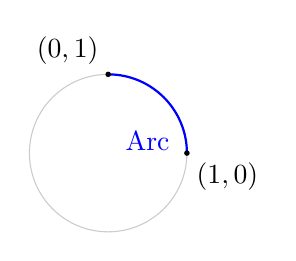
\begin{tikzpicture}
    
    % Circle
\draw[gray!40] (0,0) circle (1);

% Arc from 0 to 90 degrees
\draw[thick,blue] (1,0) arc (0:90:1);


% Mark points
\fill (1,0) circle (1pt) node[below right] {$(1,0)$};
\fill (0,1) circle (1pt) node[above left] {$(0,1)$};

% Labels
\node[blue] at (0.5,0.15) {Arc};

\end{tikzpicture}

    
\end{center}
    We will first reparameterise the curve by \[\gamma :\left [0, \frac{\pi }{2} \right ] \to [0,1], \quad \gamma (\theta) = \frac{2}{\pi} \theta, \quad g:=f \circ \gamma :\left [0, \frac{\pi}{2}\right ] \to \mathbb{R}\]
    where \[
    (f\circ \gamma ) \left ( \left[0, \frac{\pi}{2} \right]\right ) = f([0,1])
    \]
   If we show $g$ is bi-lipschitz, then $1=\dim _H(\left[0, \frac{\pi}{2} \right]) = \dim _H(f([0,1]))$. Let $\theta _1, \theta _2 \in \left[0, \frac{\pi}{2} \right ]$. Then \[
    |g(\theta _1) - g(\theta _2)| \le \text{arc length from angle } \theta _1 \text{ to } \theta _2 =  |\theta _1 - \theta _2| 
    \]
    To get a lower bound, notice that \[
    (\sin x)'' = -\sin x \le 0 \text{ on } \left[0, \frac{\pi}{2}\right]
    \]
    So $\sin x$ is concave down. That is, it lies above the chord joining any two points of its graph. Consider the chord connecting points $(0, 0)$ and $\left ( \frac{\pi}{2}, 1\right )$. The equation of this line is \[
    y = \frac{2}{\pi}x
    \]
    and this graph lies below our sine graph. That is, \[
    \sin x \ge \frac{2}{\pi} x , \quad x \in \left [ 0, \frac{\pi}{2}\right ]
    \]
    Now take $\theta_1, \theta _2 \in \left [ 0, \frac{\pi}{2}\right ]$. Then \begin{align*}
    |g(\theta _1) - g(\theta _2)| &= |(\cos \theta _1 - \cos \theta _2, \sin \theta_1 - \sin \theta _2)|      
    \\ &=\sqrt{\cos ^2 \theta _1 + \cos ^2 \theta _2 - 2 \cos \theta _1 \cos \theta _2 + \sin ^2 \theta _1 + \sin ^2 \theta _2 - 2\sin \theta_1 \sin \theta_2} \\ &=\sqrt{2-2(\cos \theta _1 \cos \theta _2 + \sin \theta _1 \sin \theta _2)} \\ & = \sqrt{2(1-\cos (\theta _1 -\theta _2))} \\ &=\sqrt{2 \left (1-2\sin ^2 \left ( \frac{\theta _1 - \theta _2}{2} \right ) +1\right )}
    \\ & = 2 \left |\sin \left ( \frac{\theta _1 - \theta _2}{2}\right ) \right| \\ & = 2 \sin \left ( \frac{|\theta _1 - \theta _2|}{2}\right ) \text{ on } \left [ 0, \frac{\pi}{2}\right ]
    \end{align*}
    But, using our lower bound for $\sin x$, we get that \[
    |g(\theta _1) - g(\theta _2)| \ge 2 \cdot \frac{2}{\pi} \left | \frac{\theta_1 - \theta _2}{2}\right | = \frac{2}{\pi} |\theta _1 - \theta _2|
    \]
    So, \[
    \frac{2}{\pi} |\theta _1 - \theta _2| \le |g(\theta_1) - g(\theta_2)| \le |\theta _1 - \theta _2| \le \frac{\pi}{2} |\theta _1 - \theta _2|
    \]
    and $g$ is bi-lipschitz, as required.

\end{ex}

~\\We can also look at the dimensions of sets in our usual real metric space, and come up with a few properties that we would expect:

\begin{lem} Consider the metric space $(\mathbb{R}, d_E)$. We have the following properties:
\begin{enumerate}
    \item $\dim_H A=0$ if $A$ is at most countable
    \item $\dim_H A \in [0,1]$ for every $A \subseteq \mathbb{R}$
\end{enumerate}
\end{lem}

\begin{proof} $ $
    \begin{enumerate}
        \item Let $\delta >0$, $s>0$ and cover $A = \bigcup \limits _{n=1}^N \{a_n\}$ for $a_n\in A$ with $N \in {\mathbb{N}^+} \cup \{\infty\}$. Then $\diam \{a_n\}=0\le \delta \text{ means } \mathcal{H}^s(A)=0$ so $\dim_H A=0$

        \item $A \subseteq \mathbb{R}$ means $0 \le \dim_H A \le \dim_H \mathbb{R} = 1$ as required.

    \end{enumerate}    
    
\end{proof}

\newpage

% \section{Mass Distributions}
% \begin{defn}
%     The \textit{support} of a Borel measure $\mu$, sometimes denoted by $\text{supp } \mu $, is defined as the smallest closed set $S$ such that \[
%     \int f d\mu = 0
%     \]
%     for every continuous function $f$ that vanishes on $S$. Equivalently, \[
%     \text{supp } \mu = \bigcap \{{F \in \mathcal{F}}: \mu (F^c) = 0 \text{ and }\mu \text{ is closed}\}
%     \]We will say that if $F \subseteq \mathbb{R}^n$ is a closed set, $\mu$ is a mass distribution on $F$ if $\text{supp }\mu \subseteq F$
% \end{defn}
% ~\\ Intuitively, the support may be thought of as the set on which $\mu$ is concentrated

% \begin{defn}
%     A Borel measure $\mu$ on $\mathbb{R}^n$, of compact support and with $0 < \mu (\mathbb{R}^n) < \infty$ is called a \textit{mass distribution}
% \end{defn}

% \begin{ex}
%     The Lebesgue measure restricted to $[0.1]$ is a mass distribution. Let $\mu : \mathcal{B}(\mathbb{R}) \to [0, \infty ]$ defined by $\mu (A) := \lambda (A \cap [0,1])$. Then we have that
%     \begin{itemize}
%         \item $\mu$ is a Borel measure
%         \item $\mu (\mathbb{R}) = \lambda ([0,1]) = 1 $
%         \item The support is the smallest closed set $F$ such that $\mu (\mathbb{R} \setminus F) = 0$. If $x \in (0,1)$, then we can find a neighbourhood of $x$ in $(0,1)$ with positive Lebesgue measure. It follows that $x \in \text{supp } \mu $. The smallest closed set containing this is $F =[0,1]$ (which clearly assigns zero measure to $\mathbb{R} \setminus F$). $F$ is compact and so $\mu$ is a mass distribution
%     \end{itemize}
% \end{ex}

% \begin{thm}{\textbf{Mass Distribution Principle}} ~\\
%     Let $\mu$ be a mass distribution on $F$ and suppose that for some $s$ there are numbers $c > 0$ and $\varepsilon>0$ such that \[
%     \mu (U) \le c\diam (U)^s
%     \]
%     for all sets $U$ with $\diam (U) \le \varepsilon$. Then \[\mathcal{H}^s(F) \ge \frac{\mu (F)}{c}\]
% \end{thm}

% \begin{proof}
%     If $\{U_i\}$ is any cover of $F$, then \[
%     0 < \mu (F) \le \mu \left ( \bigcup \limits _{i \in \mathbb{N}} U_i\right ) \le \sum \limits _{i\in \mathbb{N}} \mu (U_i) \le c \sum \limits _{i \in \mathbb{N}} \diam (U_i)^s
%     \]
%     Then for $\delta $ small enough we get $\mathcal{H}^s _\delta (F) \ge \frac{\mu (F)}{c}$ so $\mathcal{H}^s(F) \ge \frac{\mu (F)}{c}>0$
% \end{proof}
% ~\\
% The Mass Distribution Theorem gives us a way to find a quick lower esitimate for the Hausdorff dimension.
    
% \newpage 
\section{Self-Similarity}
Self-similarity captures the idea that certain subsets of $\mathbb{R}^n$ can be decomposed into smaller pieces, each of which is geometrically similar to the entire set. To formalize this, we make use of similarity transformations: mappings that preserve shape while scaling all distances by the same positive constant.

\begin{defn}
A map $S: \mathbb{R}^n \to \mathbb{R}^n$ is called a \textit{similitude} if there exists $r \in (0,1)$  such that \[
    |S(\mathbf{x}) - S(\mathbf{y})| = r |\mathbf{x}-\mathbf{y}|, \quad \text{ for all } \mathbf{x}, \mathbf{y} \in \mathbb{R}^n
    \]
    These are simply contractions in metric space $(\mathbb{R}^n, d_E)$. We call $r$ the contraction ratio of $S$.
\end{defn}

\begin{ex}
    Let $\lambda \in (0,1)$. The map $S: \mathbb{R}^n \to \mathbb{R}^n$ defined by $S(\mathbf{x})  = \lambda \mathbf{x}$ is a similitude, since, \begin{align*}
        |S(\mathbf{x}) - S(\mathbf{y})| = |\lambda \mathbf{x} - \lambda \mathbf{y}| = |\lambda| |\mathbf{x} - \mathbf{y}| = \lambda |\mathbf{x} - \mathbf{y}|
    \end{align*}
\end{ex}
~\\
For $\lambda = \frac{1}{3}$, this similitude shrinks the measure of a set in $\mathbb{R}^n$ by a factor $\frac{1}{3^n}$. The set keeps its structure and is just a smaller version.





\begin{minipage}{0.45\textwidth}
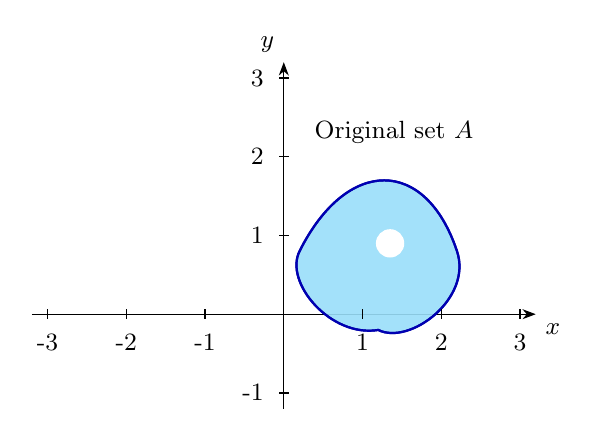
\begin{tikzpicture}[>=Stealth, every node/.style={font=\small}]
  % Axes
  \draw[->] (-3.2,0) -- (3.2,0) node[below right] {$x$};
  \draw[->] (0,-1.2) -- (0,3.2) node[above left] {$y$};

  % Original set (a fancy blob made from paths)
  \begin{scope}[shift={(1.2,0.8)}] % move the set away from origin so scaling is visible
    \fill[fill=cyan!40, draw=blue!60!black, thick, opacity=0.9]
      (-1.0,0.0) .. controls (-0.4,1.2) and (0.6,1.2) .. (1.0,0.0)
      .. controls (1.2,-0.6) and (0.4,-1.2) .. (0.0,-1.0)
      .. controls (-0.6,-1.1) and (-1.2,-0.4) .. (-1.0,0.0);

    % a hole to make it visually interesting (drawn as white)
    \fill[white] (0.15,0.1) circle(0.18);

    % outline emphasized
    \draw[blue!70!black, thick] (-1.0,0.0) .. controls (-0.4,1.2) and (0.6,1.2) .. (1.0,0.0)
      .. controls (1.2,-0.6) and (0.4,-1.2) .. (0.0,-1.0)
      .. controls (-0.6,-1.1) and (-1.2,-0.4) .. (-1.0,0.0);

    % label
    \node[above] at (0.2,1.25) {Original set $A$};
  \end{scope}



  % scale markers for reference
  \foreach \x in {-3,-2,-1,1,2,3} {\draw (\x,0.06) -- (\x,-0.06) node[below,yshift=-2pt] {\x};}
  \foreach \y in {-1,1,2,3} {\draw (0.06,\y) -- (-0.06,\y) node[left,xshift=-2pt] {\y};}

\end{tikzpicture}
    
\end{minipage}
\begin{minipage}{0.45\textwidth}

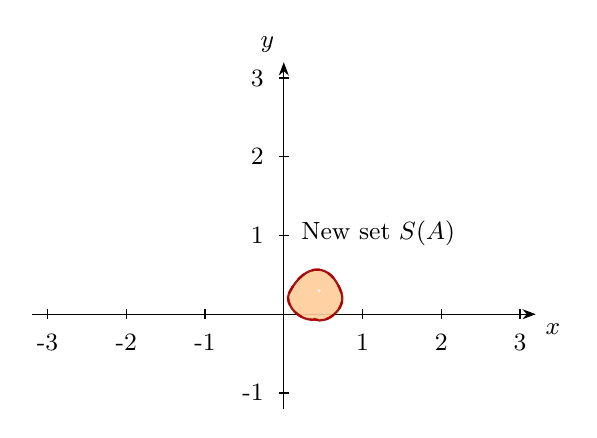
\begin{tikzpicture}[>=Stealth, every node/.style={font=\small}]
  % Axes
  \draw[->] (-3.2,0) -- (3.2,0) node[below right] {$x$};
  \draw[->] (0,-1.2) -- (0,3.2) node[above left] {$y$};


  % Scaled set: apply similitude S(x) = (1/3)x to the original shape
  % We reproduce the same path but inside a scope scaled by 1/3 about the origin.
  % Because the original was shifted, the scaled copy appears closer to origin.
  \begin{scope}[scale=1/3]
    \begin{scope}[shift={(1.2,0.8)}]
      \fill[fill=orange!40, draw=red!60!black, thick, opacity=0.9]
        (-1.0,0.0) .. controls (-0.4,1.2) and (0.6,1.2) .. (1.0,0.0)
        .. controls (1.2,-0.6) and (0.4,-1.2) .. (0.0,-1.0)
        .. controls (-0.6,-1.1) and (-1.2,-0.4) .. (-1.0,0.0);

      % small hole
      \fill[white] (0.15,0.1) circle(0.06);

      \draw[red!70!black, thick, dashed] (-1.0,0.0) .. controls (-0.4,1.2) and (0.6,1.2) .. (1.0,0.0)
        .. controls (1.2,-0.6) and (0.4,-1.2) .. (0.0,-1.0)
        .. controls (-0.6,-1.1) and (-1.2,-0.4) .. (-1.0,0.0);

    \end{scope}
  \end{scope}


  % scale markers for reference
  \foreach \x in {-3,-2,-1,1,2,3} {\draw (\x,0.06) -- (\x,-0.06) node[below,yshift=-2pt] {\x};}
  \foreach \y in {-1,1,2,3} {\draw (0.06,\y) -- (-0.06,\y) node[left,xshift=-2pt] {\y};}

  % label
    \node[above] at (1.2,0.75) {New set $S(A)$};

\end{tikzpicture}
    
\end{minipage}

~\\
We can then ask what happens when we continually apply similitudes onto a set? let's look at this example:

\begin{ex}
    Consider similitude $S: \mathbb{R} \to \mathbb{R}$ defined by $S(x) = \frac{1}{3}x$, applied repeatedly to the set $[0,1]$. The first few iterations $S^n([0,1]) := \underbrace{S(S(...S([0,1])...))}_{n \text{ times}}$ are:
\[
        S^1([0,1])  = \left [0, \frac{2}{3} \right ], \quad
    S^2([0,1])  = \left [0, \frac{2}{9} \right ], \quad
        S^3([0,1])  = \left [0, \frac{2}{27} \right ]
  \]
    It is clear that these sets shrink towards $\{0\}$. Indeed, since $S(\{0\}) = \{0\}$, the singleton $\{0\}$ is a fixed point of the transformation. More generally, we are interested in sets $A \subseteq \mathbb{R}$ that are \textit{invariant} under a similitude, i.e. satisfy $S(A) = A$.
~\\~\\ Because $S$ is a contraction, it is continuous and maps compact sets to compact sets. This suggests that the most interesting fixed points to study will be compact sets. If instead we consider unbounded sets, the situation becomes trivial: for instance, $S(\mathbb{R}) = \mathbb{R}$ and $S([0, \infty )) = [0, \infty)$. Similarly, the empty set is always a fixed point, but we set it aside as uninteresting. \\ ~\\ Now if $A$ were open and satisfied $S(A) = A$, then for any $x\in A$ with $x \ne 0$, repeated application of $S$ on $x$ forces $0 \in A$. Since $A$ is open, this would imply that intervals of the form $(-r,r)$ belong to $A$. Iterating backwards on this interval shows that $A$ must contain a larger interval, containing $(-r, r)$ (in our case, the interval $(-3r,3r)$). In fact, $A$ must be all of $\mathbb{R}$. To avoid such trivial cases, we focus instead on compact invariant sets.

\end{ex}

\begin{thm}\label{thm:homeo}
Let $S : \mathbb{R}^n \to \mathbb{R}^n$ be a similitude. Then it is a homeomorphism onto its image.
\end{thm}

\begin{proof}
A similitude is clearly continuous as a contraction. Injectivity follows from, if $S(\mathbf{x}) = S(\mathbf{y})$, then $|\mathbf{x}-\mathbf{y}| = \mathbf{0} \iff \mathbf{x}=\mathbf{y}$. Surjectivity follows from restricting its codomain to its image. So $S$ is bijective and has some inverse. Let $\mathbf{x'} = S^{-1} (\mathbf{x})$ and $\mathbf{y'} = S^{-1}(\mathbf{y})$. Then $S(\mathbf{x'}) = \mathbf{x}$ and $S(\mathbf{y'}) = \mathbf{y}$, so \[
|\mathbf{x}-\mathbf{y}| = |S(\mathbf{x'}) - S(\mathbf{y'})| = r|\mathbf{x'} - \mathbf{y'}| = r|S^{-1}(\mathbf{x}) - S^{-1}(\mathbf{y})|
\]
That is, $|S^{-1}(\mathbf{x}) - S^{-1}(\mathbf{y})| = \frac{1}{r} |\mathbf{x}-\mathbf{y}|$ and thus $S^{-1}$ is also a similitude and thus a continuous bijection. So $S$ is a homeomorphism onto its image.
\end{proof}

\begin{thm} \label{thm:compose}
Let $S_1$ and $S_2$ be two similitudes with contraction ratios $r_1$ and $r_2$. Then $S_2 \circ S_1$ is a similitude with contraction ratio $r_2r_1$
\end{thm}

\begin{proof}
We have that, for any $\mathbf{x},\mathbf{y} \in \mathbb{R}^n$, \[
|S_2 \circ S_1 (\mathbf{x}) - S_2 \circ S_1 (\mathbf{y})| = |S_2 (S_1 (\mathbf{x})) - S_2 (S_1 (\mathbf{y}))| = r_2 |S_1 (\mathbf{x}) - S_1 (\mathbf{y})| = r_2 r_1 |S_1 (\mathbf{x}) - S_1 (\mathbf{y}) |
\]
and $r_2r_1 \in (0,1)$, which completes the proof.
\end{proof}

\begin{defn}
    An Iterated Function System (IFS) is a finite collection $\mathcal{S}=\{S_k:\mathbb{R}^n \to \mathbb{R}^n\}_{k=1}^N$ of similitudes with $N\ge 2$, and contraction ratios $r_1, ..., r_N$. A non-empty compact set $K$ is invariant under $\mathcal{S}$ if $K = \bigcup \limits _{k=1}^N S_k(K)$
\end{defn}
~\\
\noindent\fbox{%
    \begin{minipage}{\textwidth}
    \textbf{Families of Similitudes:}  With only one similitude, the invariant set is usually uninteresting (e.g. $\{0\}$ in this case), using an application of the Contraction Mapping Theorem. But with two or more similitudes, rich geometric structures, such as fractals, emerge.

    \end{minipage}%
}
~\\
Before investigating invariant sets under similitudes, let's formalise the image of a compact set idea.
\begin{lem}
    For any collection $\mathcal{S}$ of finite similitudes, as described above, if $K \subseteq \mathbb{R}^n$ is compact, then $S_k(K)$ and $\bigcup \limits _{k=1}^N S_k(K)$ are compact in $\mathbb{R}^n$.
\end{lem}

\begin{proof}
    For every $1 \le k\le N$, $k \in \mathbb{N}$, $S_k$ is a contraction and thus continuous. So $S_k(K)$ is compact, and then $\bigcup \limits _{k=1}^N S_k(K)$ is compact as a finite union of compact sets. 
\end{proof}
~\\With this, we know such invariant sets can exist. We can show a much more powerful fact. The invariant sets exist, and they are unique.
\begin{thm}
    For any collection $\mathcal{S}$ of finite similitudes, as described above, there is a unique compact set invariant under $\mathcal{S}$
\end{thm}
\begin{proof}
    Since $\mathbb{R}^n$ is complete, by Theorem~\ref{thm:haus_met}, it follows that $\mathcal{K}(\mathbb{R}^n)$ is complete under the Hausdorff metric. Let $\tilde{S} : \mathcal{K}(\mathbb{R}^n) \to \mathcal{K}(\mathbb{R}^n)$ map $A \mapsto \bigcup \limits _{n=1}^N S_i(A)$. We have that, 
    \begin{align*}
        d_H(\tilde{S}(A), \tilde{S}(B)) & = d_H \left (\bigcup \limits _{n=1}^N S_i(A), \bigcup \limits _{n=1}^N S_i(B) \right ) \\ &  \le \max \limits _{1 \le i\le N}d_H(S_i(A), S_i(B)) \text{ by Theorem} ~\ref{thm:haus_additional}
    \end{align*}
We will show that each $d_H(S_i(A), S_i(B)) \le r_i d_H(A,B)$. WLOG, assume $d_H(S_i(A), S_i(B)) = d_E(S_i(A), S_i(B))$:
\begin{align*}
    d_E(S_i(A), S_i(B)) & = \sup \limits _{a\in A} \inf \limits _{b \in B}\underbrace{|S_i(a) -  S_i(b)| }_{\le r_i |a-b|} \\ & \le \sup \limits _{a\in A} \inf \limits _{b\in B} r_i |a-b|
    \\ & = r_i\sup \limits _{a\in A} \inf \limits _{b\in B} |a-b| \\ & = r_i d_E(A,B) \\ & \le r_i d_H(A,B)
\end{align*}
         So $d_H(S_i(A), S_i(B)) \le r_id_H(A,B) $ and $d_H(\tilde{S}(A), \tilde{S}(B)) \le \underbrace{(\max \limits _{1\le i \le N}r_i)} _{<1} d_H(A,B)$ .
    So $\tilde{S}$ is a contraction, and by the Contraction Mapping Theorem, there is a unique set $A \in \mathcal{K}(\mathbb{R}^n)$ such that $A = \tilde{S}(A) \iff A = \bigcup \limits _{k=1}^N S_k(A)$. Now $A \in \mathcal{K}(\mathbb{R}^n)$ implies $K$ is non-empty and compact. So $A$ is invariant under $\mathcal{S}$, and is unique.
\end{proof}



\begin{prop}\label{prop:contract}
    From the contraction mapping theorem, it follows that for any compact set $A$ and $K$ is invariant under $\mathcal{S}$, then $\tilde{S}^m(A) := \underbrace{\tilde{S} \circ \tilde{S} \circ \dots \circ \tilde{S}}_{m \text{ times}}(A) = \bigcup \limits _{i_1=1}^N \bigcup \limits _{i_1=2}^N ... \bigcup \limits _{i_m=1}^N S_{i_1}\circ S_{i_2} \circ \dots \circ S_{i_m}(A) \to K  \text{ as } m\to \infty $ (convergence with respect to the Hausdorff metric). So, we can find invariant sets by repeated iterations of our similitudes (which explains our example above for set $[0,1]$)
\end{prop}
~\\So far, a set that is invariant under a finite collection of similitudes can be thought of as being composed of ``smaller copies of itself" - the images under the similitudes. At this stage, we have not specified how these copies might overlap. To capture the idea of a truly self-similar set, we generally require that these copies overlap as little as possible, and we use measures to quantify and formalize this notion:

\begin{defn}
    Let $K$ be the unique invariant set under $\mathcal{S} = \{S_i\}_{i=1}^N$, and $s = \dim _H K$. Then $K$ is self-similar if \[\mathcal{H}^s(S_i(K) \cap S_j(K)) = 0\] for $ i \ne j$ and $1\le i,j \le N$, $i,j \in \mathbb{N^+}$
\end{defn}
~\\
It is enough for the similarity components to overlap only on a set of measure zero. However, this definition requires computing the Hausdorff dimension and evaluating the Hausdorff measure for every pair $i$ and $j$, which makes it difficult in practice. For this reason, we will introduce a more convenient and stronger notion of self-similarity, known as the \textit{Open Set Condition} that uses the \textit{similarity dimension} of a family of similitudes

\begin{defn}
    Let $\mathcal{S}$ be a finite family of similitudes. If \[
    \sum \limits_{i=1}^N r_i^D = 1
    \]then we call $D$ the \textit{similarity dimension} of $\mathcal{S}$. We will denote it by $\dim _S\mathcal{S} $.
\end{defn}

\newpage

\begin{defn}{\textbf{OSC: The Open Set Condition}} ~\\
    A finite collection of similitudes $\mathcal{S}$ satisfy the \textit{Open Set Condition} if there exists a nonempty open set $O$ such that \[\bigcup \limits _{i=1}^N S_i(O) \subseteq O \text{ and } S_i(O) \cap S_j(O) = \emptyset \text{ for } i \ne j, 1\le i,j\le N, i,j \in \mathbb{N}^+\]Furthermore, we may assume $O$ is bounded, as if it is unbounded we simply take a bounded subset of it.
\end{defn}

\noindent\fbox{%
    \begin{minipage}{\textwidth}
        \textbf{Why the Open Set Condition?} The OSC ensures the similarity components overlap minimally, allowing us to calculate dimensions using a simple formula rather than complex measure-theoretic arguments. This is proven in the next theorem.
    \end{minipage}%
}

\begin{thm}~\label{thm:haus_similar_connection}
    If $\mathcal{S}$ satisfies the OSC, then the invariant set $K$ of $\mathcal{S}$ is self-similar and $0 < \mathcal{H}^s(K)<\infty$ where $s$ is the unique number for which \[
    \sum \limits _{i=1}^N r_i^s = 1
    \]
    That is, $\dim _S \mathcal{S} = \dim _H K$ (the similarity dimension is the same as the Hausdorff dimension).
\end{thm}
\begin{proof}
    See Appendix C
\end{proof}
~\\This theorem provides us a way to find the dimension of a fractal $K$. If we can find a collection $\mathcal{S}$ of finite similitudes such that $K$ is invariant, and show that the collection of similitudes satisfies the Open Set Condition, then the dimension is simply the solution to \[
\sum \limits _{i=1}^N r_i^s = 1
\]
~\\
Note that while this theorem is strong, we can still have self-similar sets whose similitudes do not satisfy the Open Set Condition and in this case we cannot use this theorem. What we will show is a set of similitudes that fail OSC.

\begin{ex}
Consider similitudes $S_1(x) = \frac{1}{4}x$ and $S_2(x) = \frac{1}{2}x $. Then $S_1 (\{0\}) \cup S_2 (\{0\}) = \{0\}$ so $\{0\}$ is the unique invariant set under $\{S_1,S_2\}$. Suppose that these satisfy OSC, that is, there is a nonempty open set $O$ such that $S_1(O) \subseteq O$ and $S_2 (O) \subseteq O$ and $S_1 (O) \cap S_2 (O) = \emptyset$. Then $\frac{1}{2} O \subseteq O$ and it implies that $0 \in O$ (take any $x \in O$, then $\frac{1}{2}x \in O \Rightarrow \frac{1}{4}x \in O ... $). But then $0 \in S_1 (O) \cap S_2(O)$, a contradiction. Thus the similitudes $\{S_1, S_2\}$ fail OSC. We will show that the dimensions differ.
We have that $\dim _H (\{0\})) = 0$, but $\dim _S \{S_1,S_2\} =: d \iff \left (\frac{1}{2} \right )^d + \left ( \frac{1}{4}\right )^d = 1$ whose solution is \[
d = -\frac{\ln((\sqrt{5} - 1)/2)}{\ln 2}
\]
\end{ex}
~\\As explained by 3Blue1Brown, the similarity dimension comes from the idea that the dimension of a set reflects how the number of small pieces needed to cover it grows as you zoom in: if shrinking the scale by a factor of $r$ requires $N$ self-similar copies, then the dimension is the solution of $N \cdot r^d = 1$. An example of this is, if we shrink an interval by $\frac{1}{2}$, we need $2^1$ copies to cover it again so its dimension is one. If we shrink a square by $\frac{1}{2}$, we need $4 = 2^2$ copies to cover it again, so it is 2 dimensional. This works perfectly when the pieces really are independent, because each copy contributes separately to covering the set. The Open Set Condition ensures that the pieces don't overlap too much and thus this holds. But if the OSC fails, some of the smaller copies overlap heavily, so you don't actually need all $N$ of them to cover the set. In that case the similarity dimension is inflated, while the Hausdorff dimension is lower.

\newpage
\begin{cor}
    If $\mathcal{S}$ satisfies the Open Set Condition and $r_1=r_2=...=r_N=r$, then $\dim_H K = -\frac{\ln N}{\ln r}$
\end{cor}
\begin{proof}
    Our dimension $s$ is the unique solution to \[
    \sum \limits _{i=1}^N r^s = 1 \iff Nr^s = 1\iff r^s = \frac{1}{N} \iff s = \frac{\ln \left ( N^{-1}\right )}{\ln r} = -\frac{\ln N}{\ln r}
    \]
\end{proof}
~\\
One final property, which we will use when looking at fractals, is that similitudes preserve arbitrary intersections. That is, \begin{thm}\label{thm:pres_sim}
    Let $S: \mathbb{R}^n \to \mathbb{R}^n$ be a similitude, and $\{A_i\}_{i\in I}$ be a family of subsets of $\mathbb{R}^n$ (for an arbitrary index set $I$). Then \[
    S \left ( \bigcap \limits _{i \in I} A_i\right ) = \bigcap \limits _{i \in I} S(A_i)
    \]
\end{thm}

\begin{proof}
    Clearly \[
    \bigcap \limits _{i \in I } A_i \subseteq A_i \quad \text{for each } i \in I \text{ so }S \left ( \bigcap_{i \in I} \limits A_i\right )\subseteq \bigcap \limits _{i \in I} S(A_i)
    \]
    In Theorem~\ref{thm:homeo}, we showed $S$ is injective. Take any $\mathbf{y} \in \bigcap \limits _{i \in I} S(A_i)$. Then $\mathbf{y} \in S(A_i)$ for each $i \in I$. For each $i \in I$, there is some $\mathbf{x}_i \in A_i$ such that $S(\mathbf{x}_i) = \mathbf{y}$ But, $S$ being injective means $ \mathbf{x}_i=\mathbf{x}_j =: \mathbf{x} $ for every $i,j \in I$. So $\mathbf{x} \in A_i$ for each $i\in I$ and \[
    \mathbf{x} \in \bigcap \limits _{i \in I}A_i \text{ so } \mathbf{y} \in S \left ( \bigcap \limits _{i \in I}A_i\right )
    \]
    which completes the proof.
\end{proof}

\newpage

%
%\section{Topological Dimension}
%Before diving into specific fractals, we pause to formally define what makes a set a fractal. This requires understanding the topological dimension of a set, which captures our intuitive notion of dimension through covering properties.
%~\\ ~\\ Suppose we are in a topological space $(X, \tau)$.
%\begin{defn}
%    Let $\mathcal{U} = \{U_i\}_{i \in I}$ be an open cover of $X$. A \textit{refinement} of an open cover $\mathcal{U}$ is another open cover $\mathcal{V} = \{V_j\}_{j \in J}$ such that for every $V_j \in \mathcal{V}$, there exists some $U_i \in \mathcal{U}$ with $V_j \subseteq U_i$
%    
%\end{defn}
%~\\This shows a refinement of the open sets (each a different colour) covering the border of a circle.
%
%\begin{center}
%    \includegraphics[scale = 0.4]{assets/circle_big.png}
%\end{center}
%
%\begin{defn}
%    We say $\dim_H(X) \le n$ if every finite open cover $\mathcal{U}$ of $X$ has a finite open refinement $\mathcal{V}$ such that no point of $X$ is contained in more than $n+1$ sets of $\mathcal{V}$. The smallest such $n \in \mathbb{Z}$ is called the \textit{Lebesgue covering dimension}, or also called the \textit{Topological dimension} of $X$. We will denote it as \[
%    \dim _T(X) = n
%    \]
%    If no such $n$ exists, we say $\dim_T (X) = \infty$. If $A \subseteq X$, we find the topological dimension by considering the topological space $A$, equipped with the subspace topology. By convention, $\dim _T(\emptyset) = -1$.
%\end{defn}
%~\\
%For the image above, the refinement covers (since they are open) must intersect. So for this specific cover, no point on the circle is contained in more that $1+1 = 2$ sets in the refinement. This hints at the circle being 1 dimensional.
%~\\~\\
%The topological dimension reflects how many independent directions are available within a space. On a line (1D), you can move only forward or backward; on a plane (2D), you add left and right; in 3D space, up and down provide a third direction. More generally, the dimension describes how the space looks locally: zooming in on a curve resembles a line (1D), on a surface resembles a disk (2D), and so forth. Formally, this is captured using open covers. For a 1D curve, small neighborhoods can be refined so that at most two overlap at any point, reflecting its single direction of movement. On a 2D surface, neighborhoods may require up to three overlapping at a point, corresponding to two independent directions. Thus, the topological dimension measures the minimal number of overlaps needed—and this aligns with our intuitive sense of how many directions a space offers locally.
%~\\~\\
%let's look at a one quick example. We will look at more complex examples when we look at fractals.
%\begin{ex}
%    Consider the standard topological space on $\mathbb{R}$ and take any $x \in \mathbb{R}$. The subspace topology is then $\tau _x = \{\emptyset, \{x\}\}$. Let $\mathcal{U}$ be an open cover of $\{x\}$. Then there is some $U_i = \{x\}$. By considering refinement $\mathcal{V} = \{U_i\}$, then $x$ is contained in only $1$ set of $\mathcal{V}$ and thus $\dim _T(\{x\}) = 0$
%\end{ex}
%~\\
%The reason for looking at the topological dimension is to give a formal, rigorous definition of a fractal
%\begin{defn}
%    A \textit{fractal} is a set $A$ in metric space $(X,d)$, and its induced topological space $(X, \tau )$, such that \[
%    \dim _T(A) < \dim _H(A)
%    \]
%    that is, its Hausdorff dimension exceeds its Topological dimension.
%\end{defn}
%
%\noindent\fbox{%
%    \begin{minipage}{\textwidth}
%        The sets we'll study next all satisfy $\dim_T(K) < \dim_H(K)$, making them genuine fractals — objects whose geometric complexity exceeds their topological structure.
%    \end{minipage}%
%}
%~\\~\\
%\textbf{Interesting Fact:} It can actually be shown that in a separable metric space $(X,d)$, we have that \[
%\dim _T(A) \le \dim _H(A)
%\]
%So if $\dim _H(A) \notin \mathbb{Z}$, then it immediately follows that $\dim _T(A) < \dim _H (A)$ and our set $A$ is a fractal. We do not prove this and will not use it in later sections.
%
%\newpage

\section{The Cantor Set}

\begin{minipage}{0.6 \textwidth}
We start by describing the construction of the Cantor Set
\small{
\begin{itemize}
    \item Start with the closed interval $C_0 = [0,1]$.
    \item Remove the open middle third $(\tfrac{1}{3}, \tfrac{2}{3})$, leaving  $C_1 = \left[0, \tfrac{1}{3}\right] \cup \left[\tfrac{2}{3}, 1\right]$.
    \item From each remaining interval, again remove the open middle third. This gives $C_2 = \left[0, \tfrac{1}{9}\right] \cup \left[\tfrac{2}{9}, \tfrac{1}{3}\right] \cup \left[\tfrac{2}{3}, \tfrac{7}{9}\right] \cup \left[\tfrac{8}{9}, 1\right]$.
    \item Repeating this process indefinitely, we obtain a nested sequence of sets $C_0 \supset C_1 \supset C_2 \supset \cdots$, where $C_n$ is the result after $n$ steps.
    \item More formally, define $C_n := \frac{C_{n-1}}{3} \cup \left (\frac{1}{3}  + \frac{C_{n-1}}{3}\right)$, $C_0 := [0,1]$
    \item The Cantor set is defined as the limit of this process:
    \[
        \mathcal{C} := \bigcap_{n=0}^{\infty} C_n.
    \]
    \item The Cantor Set is not empty (for example, $1 \in \mathcal{C}$)
\end{itemize}}
\end{minipage}%
\begin{minipage}{0.39 \textwidth}
  \begin{center}
\includegraphics[width = \textwidth]{assets/cantor.png}    
\end{center}
\end{minipage}

\subsection{The Hausdorff Dimension of The Cantor Set Directly}

We will prove that $\dim_H \mathcal{C} = \frac{\ln 2}{\ln 3}$. By construction, $\mathcal{C} \subseteq C_n$ for each $n \in \mathbb{N}_0$. $C_n$ contains  $2^n$ intervals $\{I_{n, m}\}_{m=1}^{2^n}$ with $\diam(I_{n, m}) = 3^{-n}$ and $C_n = \bigcup \limits _{m=1}^{2^{n}}I_{n,m}$. Take $\delta >0$ and $n$ large enough such that $3^{-n} \le \delta $. Thus

\[\mathcal{H}_{\delta}^d(\mathcal{C})  \le \mathcal{H}_\delta ^d(C_n) \le \sum \limits _{m=1}^{2^{n}} (\diam (I_{n,m}))^d=\sum \limits  _{m=1}^{2^{n}} (3^{-n})^d= (3^{-nd})(2^{n})= \left (\frac{2}{3^d} \right)^{n}\]
If $\frac{2}{3^d} < 1$, then as $n \to \infty$, $(\frac{2}{3^d})^n \to 0$ and so $\mathcal{H} ^d(\mathcal{C})=0$. We have that \[\frac{2}{3^d} < 1 \iff 3^d > 2 \iff d > \frac{\ln 2}{ \ln 3}\]
From this we deduce $\dim _H \mathcal{C} \le \frac{\ln 2}{\ln 3} =: d$. Let $\{E_n\}_{n\in \mathbb{N}^+}$ be a covering for $\mathcal{C}$ with $\diam (E_{n})< \frac{1}{3}$ (which clearly exists). Notice $C_n$ is compact, as a union of finite intervals (which are compact). It follows that $\mathcal{C} = \bigcap \limits _{n=0}^\infty C_n$ is compact. So $\{E_n\}_{n\in \mathbb{N}^+}$ has a finite subcovering $\{E_{n_k}\}_{k=1}^N$ that covers $\mathcal{C}$. We may also assume that $E_{n_k} \cap \mathcal{C} \ne \emptyset $, otherwise we remove $E_{n_k}$ from our family of sets. Clearly \[
\sum \limits _{n\in \mathbb{N}^+}\diam (E_n)^d \ge \sum \limits _{k=1 }^N \diam (E_{n_k})^d
\]
For each $k=1,...,N$, let  $m_k \in \mathbb{N}^+ \text{ be such that }3^{-(m_k+1)} \le \diam (E_{n_k})< 3^{-m_k}$.
Because $E_{n_k} \cap \mathcal{C} \ne \emptyset$, clearly $E_{n_k}$ intersects at least one interval in $C_{n_k}$. It cannot intersect more than one interval, because otherwise, if there were points $x, y$ in different intervals in $C_n$ and $x,y \in E_{n_k}$, then $\diam (E_{n_k}) \ge |x-y| \ge 3^{-m_k}$, with each interval being at least $3^{-m_k}$ away from each other. By assumption, this cannot happen. So $E_{n_k}$ intersects exactly one interval $I_{n_k, p}$ in $C_n$, with $p \in \{1,2,...,2^{n_k}\}$. 
~\\~\\
But then in $C_{m_k+1}$, interval $I_{m_k, p}$ splits into 2 smaller intervals, and thus $E_{n_k}$ intersects at most $2^{1}$ intervals. Recursively, for any $x \ge m_k,\  x \in \mathbb{N}$, $E_{n_k}$ intersects at most $2^{x-m_k}$ intervals in $C_x$. Notice that \[\diam(E_{n_k})^d \ge 3^{-d(m_k+1)}=(3^{d})^{-1}(3^{d})^{-m_k}=2^{-1}2^{-m_k}\] So $2^x \diam (E_{n_k})^{d} \ge 2^{x-m_k} 2^{-1}$.
Now let $M = \max \limits _{\substack{1\le k\le N \\ k \in \mathbb{N}}}m_k$. Let $M_k$ be the number of intervals $E_{n_k}$ intersects with in $C_M$. We have shown $M_k \le 2^{M-m_k}$. Since $\{E_{n_k}\}$ covers $\mathcal{C}$, and the endpoints of every interval are in $\mathcal{C}$, every interval intersects some $E_{n_k}$ and thus $\sum\limits _{k=1}^{N} M_k \ge 2^{M}$. Now \[\sum \limits _{k=1}^N(\diam (E_{n_k}))^d =\sum \limits _{k=1}^N2^M \diam (E_{n_k})^d \cdot 2^{-M} \ge 2^{-1} 2^{-M}\sum \limits _{k=1}^N2^{M-m_k}\ge2^{-1}2^{-M}\sum \limits _{k=1}^NM_k \ge 2^{-1}2^{-M}2^M = \frac{1}{2}\]Thus \[\frac{1}{2} \le \mathcal{H}^d(\mathcal{C}) \le 1 \text{ and so } d = \dim \mathcal{C}\]

\subsection{The Hausdorff Dimension of the Cantor Set using Self-Similarity}
Calculating the Hausdorff dimension analytically, as done above, is clearly a lot of work. As will be the case with some fractals, we can use the fact the fractal is self-similar to come up with a recurrence relation that describes it. In the case of the Cantor Set, its iterations are described by: $C_0 = [0,1]$, and 
\[
C_n = \frac{C_{n-1}}{3} \cup \left (\frac{1}{3}  + \frac{C_{n-1}}{3}\right)
\]
Define similitudes $S_1:\mathbb{R} \to \mathbb{R}$ and $S_2:\mathbb{R} \to \mathbb{R}$ by $S_1(x) = \frac{1}{3}x$ and $S_2(x) = \frac{1}{3}x + \frac{2}{3}$. Then our contraction ratios are both $\frac{1}{3}$. We then have that \[
\mathcal{C} = \bigcap \limits _{n \in \mathbb{N}_0} C_n = \bigcap \limits _{n \in \mathbb{N}^+}C_n = \bigcap \limits _{n \in \mathbb{N}^+}\big [ S_1(C_{n-1}) \cup S_2(C_{n-1})\big] = \bigg [ \bigcap \limits _{n \in \mathbb{N}^+}S_1(C_{n-1})\bigg ] \cup \bigg [ \bigcap \limits _{n \in \mathbb{N}^+}S_2(C_{n-1})\bigg ] \]By Theorem~\ref{thm:pres_sim}, similitudes preserve intersections and so \[
\mathcal{C} = 
\bigg [ S_1 \left ( \bigcap \limits _{n \in \mathbb{N}^+}C_{n-1} \right )\bigg ] \cup \bigg [ S_2 \left ( \bigcap \limits _{n \in \mathbb{N}^+} C_{n-1} \right )\bigg ] = S_1 (\mathcal{C}) \cup S_2(\mathcal{C})
\] $\mathcal{C}$ is compact, so $\mathcal{C}$ is the unique set invariant under $\{S_1, S_2\}$. To show $\mathcal{C}$ is self-similar, we use (OSC). We need to find a non-empty open set $O$ such that $S_1(O) \cup S_2(O) \subseteq O$ and $S_1 (O) \cap S_2(O) = \emptyset$. This is simple, we just take open set $O = (0,1)$ with $S_1(O) = \left (0, \frac{1}{3}\right)$ and $S_2(O) = \left (\frac{2}{3}, 1 \right )$. By Theorem~\ref{thm:haus_similar_connection}, $\dim_H \mathcal{C} = \dim _S \{S_1,S_2\} =: d$ is the unique number such that \[\frac{2}{3^d} = 1 \iff d = \frac{\ln 2}{\ln 3}\]
This is the technique we will generally use for finding the dimension of a fractal.

\subsection{Uncountability of the Cantor Set}

A remarkable property of the Cantor set is that, since its dimension is strictly less than $1$, we have 
\[
\lambda_{1}(C) = \mathcal{H}^{1}(C) = 0.
\] 
Despite this, the set is uncountable. Furthermore, it contains no intervals, making it an uncountable set with measure zero and no intervals. Before proving its uncountability, we first establish a few key properties.

\newpage

\begin{thm}\label{thm:b-ary}
    Given an integer $b \geq 2$, every real number $x \in [0,1]$ can be written as
    \[
        x = \sum_{n=1}^\infty \frac{x_n}{b^n},
    \]
    where each digit $x_n \in \{0,1,\dots,b-1\}$. In this case, we write $x = (0.x_1x_2\ldots)_b$ and call this the \emph{$b$-ary expansion} of $x$ (with $b=2$ being binary, $b=3$ ternary, and $b=10$ the usual decimal expansion).
\end{thm}

\begin{proof}
    First consider the case $x=1$. If we set $x_n = b-1$ for all $n \geq 1$, then
    \[
        \sum_{n=1}^\infty \frac{x_n}{b^n} 
        = \sum_{n=1}^\infty \frac{b-1}{b^n} 
        = (b-1) \sum_{n=1}^\infty \left(\frac{1}{b}\right)^n
        = (b-1)\,\frac{1/b}{1-1/b} 
        = 1,
    \]
    as required. Henceforth, assume $x < 1$. Set $y_1 := x$. Define
    \[
        Y_1 := \{n \in \mathbb{N}_0 : \tfrac{n}{b} \leq y_1\}.
    \]
    Since $0 \in Y_1$ and $\tfrac{b}{b} = 1 > y_1$, the set $Y_1$ is finite and has a largest element, which we denote by $x_1$. Then $0 \leq x_1 \leq b-1$. Define
    \[
        y_2 := y_1 - \frac{x_1}{b}.
    \]
    By construction, $\tfrac{x_1}{b} \leq y_1 < \tfrac{x_1+1}{b}$, hence
    \[
        0 \leq y_2 < \frac{1}{b}.
    \]
    Inductively, for $k -1 \ge 1$, suppose $y_{k-1}$ has been defined with $0 \leq y_{k-1} < \tfrac{1}{b^{k-2}}$. Set
    \[
        Y_k := \{n \in \mathbb{N}_0 : \tfrac{n}{b^k} \leq y_k\}, 
        \qquad x_k := \max Y_k,
    \]
    and define
    \[
        y_k := x - \sum_{n=1}^{k-1} \frac{x_n}{b^n} = y_{k-1} - \frac{x_{k-1}}{b^{k-1}}
    \]
    Then $0 \leq y_k < \tfrac{1}{b^{k-1}}$ and $Y_k$ is nonempty (since $0 \in Y_k$) and bounded (since $y_k < \tfrac{b}{b^k}$). Thus each $x_k$ is well defined with $0 \leq x_k \leq b-1$. Now consider the partial sums
    \[
        s_m := \sum_{n=1}^m \frac{x_n}{b^n}.
    \]
    These form an increasing sequence with $s_m \leq x$ for all $m \in \mathbb{N}^+$. Moreover,
    \[
        0 \le x - s_m = y_{m+1} < \frac{1}{b^m} \to 0 \text{ as } m \to \infty
    \]
    So $s_m \to x$ as $m \to \infty$. Hence
    \[
        x = \sum_{n=1}^\infty \frac{x_n}{b^n},
    \]
    which completes the proof.
\end{proof}
\begin{ex}
    The $b$-ary expansion (as a sequence) of a number need not be unique. In ternary, \[
    \frac{1}{3} = (0.1000...)_3 \text{ and } (0.0222...)_3 = \sum \limits _{n=2}^{\infty} \frac{2}{3^n} = 2 \sum \limits _{n=2}^{\infty} \frac{1}{3^n} = 2 \cdot \frac{1/9}{1-1/3} = 2\cdot \frac{1}{6} = \frac{1}{3}
    \]
\end{ex}
\newpage
\begin{thm}\label{thm:cantor_form}~\\
    The Cantor set $\mathcal{C}$ is the set of numbers in $[0,1]$ such that there exists a ternary expansion that only contains the digits $0$ and $2$, i.e., \[
    \mathcal{C} = \{x = (0.x_1x_2x_3...)_3 : x_n \in \{0,2\}, \forall n \in \mathbb{N}^+\}
    \]
\end{thm}

\begin{proof}
Take some $x \in \mathcal{C}$ and let $x = (0.x_1x_2x_3...)_3$ be a ternary expansion of $x$, that exists by Theorem~\ref{thm:b-ary}. We will show, by induction, that for $N \in \mathbb{N}^+$, 
    \begin{enumerate}
        \item $x_N$ determines the interval in $C_N$ that $x$ is in
        \item $x_m \in \{0,2\}$ for every $1 \le m \le N$
        \item The endpoints of the interval in $C_N$ containing $x$ has $(0.x_1x_2...x_N000...)_3$ as its left endpoint, and $(0.x_1x_2...x_N222...)_3$ for its right endpoint.
    \end{enumerate}
    For the base case, $N=1$, we have that \[
    x \in \left [ 0, \frac{1}{3}\right] \text{ or } x \in \left [ \frac{2}{3}, 1\right ], \quad \text{since } x \in \mathcal{C} \text{  so  } x \in C_1
    \]
So if $x_1 = 1$, then \[
  \sum \limits _{n=1}^{\infty } \frac{x_n}{3^n}  = \frac{1}{3} +  \sum \limits _{n=2}^{\infty } \frac{x_n}{3^n} 
\]
So \[
\frac{1}{3} \le x \le \frac{1}{3} + \sum \limits _{n=2}^\infty \frac{2}{3^n} = \frac{2}{3}
\]
So the only possibility is \[
x = \frac{1}{3} = (0.0222...)_3 \text{ or } x = \frac{2}{3} = (0.200...)_3
\]
and both have a ternary expansion containing only zeroes and twos, so we can ignore these cases in this proof. If $x_1 = 0 $, then $x \le (0.0222...)_3 = \frac{1}{3}$. If $x_1 = 2$, then $x \ge \frac{2}{3}$. So
\begin{enumerate}
    \item $x_1$ determines the interval in $C_1$ that $x$ is in
    \item $x_1 \in \{0,2\}$
    \item Finally, for interval $ \left[0, \frac{1}{3} \right ]$ (where $x_1 = 0$), we have $0 = (0.00...)_3$, $\frac{1}{3} = (0.0222...)_3$, and, for interval $\left [ \frac{2}{3}, 1\right ]$ (where $x_1 = 2$), $\frac{2}{3} = (0.2000...)_3$ and $1 = (0.22222...)_3$. So every endpoint in $C_1$ has ternary expansions in the specified form, so specifically the interval $x$ is in has the required form.
\end{enumerate}
Now assume that for $n \ge 1$, the inductive hypothesis holds. 
Since $x \in C_n$, let $a = (0.x_1x_2...x_n00...)_3$ be the left endpoint of the interval $x$ is in in $C_n$. Then $ x  \in \left [a, a+3^{-n} \right ] $ (as intervals in $C_n$ have length $3^{-n}$). But $x \in C_{n+1}$ so \[
x \in \left [a, a+3^{-n-1} \right ] \text{ or } x \in \left [ a + 2 \cdot 3^{-n-1}, a + 3^{-n}\right ]
\]
If $x_{n+1} = 1$, then \[
  \sum \limits _{k=1}^{\infty } \frac{x_k}{3^k}  = \sum \limits _{k=1}^{n} \frac{x_k}{3^k} + \frac{1}{3^{n+1}} + \sum \limits _{k=n+2}^{\infty} \frac{x_k}{2^k}
\]
and \[
a  + \frac{1}{3^{n+1}} + 0\le \sum \limits _{k=1}^{n} \frac{x_k}{3^k} + \frac{1}{3^{n+1}} + \sum \limits _{k=n+2}^{\infty} \frac{x_k}{3^k} \le a + \frac{1}{3^{n+1}} + \sum \limits _{k = n+2}^{\infty } \frac{2}{3^k}
\]
So \[
a + 3^{-n-1} \le x \le a+2\cdot 3^{-n-1}
\]
Again, $x$ must be on the boundary. But we have that \[
a + 3^{-n-1} = a+ \frac{1}{3^{n+1}} = (0.x_1x_2...x_n100...)_3 = (0.x_1x_2...x_n02222...)_3
\]
and 
\[
a + 2 \cdot 3^{-n-1} = a+ \frac{2}{3^{n+1}} = (0.x_1x_2...x_n200...)_3 
\]
Both of which have a ternary expansion containing only zeroes and twos, and thus can be ignored. Notice that even the endpoints satisy the left and right endpoint form required. So $x_{n+1} \in \{0,2\}$. Now if $x_{n+1} = 2$, then $x \ge (0.x_1x_2...x_{n}200...)_3 = a + 2 \cdot 3^{-n-1}$. If $x_{n+1} = 0$, then $x \le (0.x_1x_2...x_n0222...)_3 = a + \cdot 3^{-n-1}$. So
\begin{enumerate}
    \item $x_{n+1}$ determines which interval $x$ is in in $C_{n+1}$
    \item $x_{m} \in \{0,2\}$ for all $1 \le m \le n+1$
    \item Finally, the endpoints of intervals follow from the above calculation and the inductive hypothesis.
\end{enumerate}
which completes the inductive proof and shows that $x$ has a ternary form consisting of only zeroes and twos.
~\\ ~\\Now suppose that $x = (0.x_1x_2...)_3$ is a number with a ternary expansion containing only zeroes and twos. We will show by induction that $x \in C_n$, and that $(0.x_1x_2...x_n00...)_3$ is the left endpoint of the interval containing $x$ in $C_n$, for every $n$. For $n=0$, by definition, $x \in [0,1]$ and the left endpoint has the form $(0.00...)_3$. So assume the inductive hypothesis holds for some $n \ge 0$. Then $x \in [a, a+3^{-n}]$ for some $a \in \mathbb{R}$. Then \[
a = (0.x_1x_2...x_n000...)_3 
\]
If $x_{n+1} = 2$, then $a + 3^{-n} \ge x \ge (0.x_1x_2...x_{n+1}00...)_3 = a+2 \cdot 3^{-n-1}$ and so $x \in C_{n+1}$. If $x_{n+1} = 0$, then \[
a = (0.x_1x_2...x_{n+1}00...)_3\le x = \sum \limits _{k=1}^{n} \frac{x_n}{3^n} + \sum \limits _{k=n+2}^\infty \frac{x_n}{3^n} \le a + \frac{1}{3^{n+1}}
\]
as required. So $x \in \mathcal{C}$.

\end{proof}
~\\As a part of the proof, we have actually shown 
\begin{lem}\label{lem:endpoints}
    Let $x \in \mathcal{C}$ and $x=(0.x_1x_2...)_3$ be its ternary expansion containing only zeroes and twos (which exists by Theorem~\ref{thm:cantor_form}). Then, for any $n \in \mathbb{N}_0$, the interval in $C_n$ containing $x$ is \[
    \left [(0.x_1x_2...x_n00...)_3, (0.x_1x_2...x_n22...)_3 \right]
    \]
\end{lem}
~\\ Our means of showing the Cantor Set is uncountable is to construct a surjective map $f: \mathcal{C} \to [0,1]$. We thus want to ensure that the ternary expansion of a number in the Cantor Set is unique, so our map is well defined.

\begin{lem}\label{lem:well-defined-cantor}
    The ternary expansion of any $x \in \mathcal{C}$ containing only zeroes and twos is unique.
\end{lem}

\begin{proof}
    Let $x=(0.a_1a_2...)_3 = (0.b_1b_2...)_3 \in \mathcal{C}$ be two ternary expansions containing only zeroes and twos. By Lemma~\ref{lem:endpoints}, we know that, for each $n \in \mathbb{N}_0$, $(0.a_1a_2...a_n00...)_3 = (0.b_1b_2...b_n00...)_3$, is the left endpoint of the interval in $C_n$ containing $x$. Clearly then $(0.a_100...)_3 = (0.b_10...)_3$ so $a_1 = b_1$ (as the left endpoint in $C_1$).  For $n \ge 2$, we have \[
    (0.0...0a_n0...)_3 = (0.a_1a_2...a_n00...)_3  - (0.a_1a_2...a_{n-1}00...)_3 = (0.b_1b_2...b_n00...)_3  - (0.b_1b_2...b_{n-1}00...)_3  = (0.0...0b_n0...)_3
    \]
    So $a_n = b_n$ for all $n \in \mathbb{N}^+$.
\end{proof}
~\\We can now finally show the Cantor Set is uncountable

\begin{thm}~\\
    The Cantor Set is uncountable. More specifically, $|\mathcal{C}| = |[0,1]| = \mathfrak{c}$
\end{thm}

\begin{proof}
    Consider the map $f: \mathcal{C} \to [0,1]$ defined by \[
    f((0.x_1x_2x_3...)_3) = \frac{1}{2} \sum \limits _{n=1}^\infty \frac{x_n}{2^n}
    \]
    using its ternary expansion with only zeroes and twos (from Theorem~\ref{thm:cantor_form}). Lemma~\ref{lem:well-defined-cantor} shows this is well-defined. ~\\
    We claim this is surjective. Let $y = (0.y_1y_2y_3...)_2 \in [0,1]$. For each $n\in \mathbb{N}^+$, let $x_n = 2y_n$. Then $x_n \in \{0,2\}$, so $x = (0.x_1x_2x_3...)_3 \in \mathcal{C}$ and \[
    f(x) = \frac{1}{2}\sum \limits _{n=1}^\infty \frac{x_n}{2^n} = \frac{1}{2}\sum \limits _{n=1}^\infty \frac{2y_n}{2^n} = \sum \limits _{n=1}^\infty \frac{y_n}{2^n} = y
    \]
    So $f$ is surjective and $|\mathcal{C}| \ge |[0,1]|$. Then $\mathcal{C} \subseteq [0,1]$ implies $|\mathcal{C} | \le |[0,1]|$ meaning $|\mathcal{C} | = |[0,1]|$
    
\end{proof}

\begin{thm}\label{thm:cantor_interval}
    The Cantor set contains no interval of positive length (i.e., no nontrivial intervals)
\end{thm}
\begin{proof}
    Assume otherwise, that the Cantor set has an interval $I$ of length $\varepsilon > 0$. Then, taking $N$ large enough such that \[
    \frac{1}{3^n} < \varepsilon
    \] means that $C_N$ consists of intervals of length $3^{-N}$ and so $I \not \subseteq C_N$, a contradiction.
\end{proof}
~\\This theorem allows us to show that the Cantor Set is totally disconnected. For that, we need:

\begin{lem}
\label{lem:connected-subsets-are-intervals}
Every connected subset \(C\subseteq\mathbb{R}\) (with the subspace topology) is an interval. That is, if \(x,y\in C\) and \(x<y\), then \([x,y]\subseteq C\).
\end{lem}

\begin{proof}
Suppose \(C\subseteq\mathbb R\) is connected and let \(x,y\in C\) with \(x<y\). If there exists \(z\in (x,y)\) with \(z\notin C\), then
\[
U:=(-\infty,z)\cap C,\qquad V:= (z,\infty)\cap C
\]
are two disjoint, nonempty sets whose union equals \(C\). But this contradicts that $C$ is connected. So $[x,y] \subseteq C$.
\end{proof}

\begin{prop}
\label{prop:closed-no-intervals-totally-disconnected}
Let \(F\subseteq\mathbb{R}\) be a closed set. If \(F\) contains no nontrivial interval (some interval $[a,b]$ with $a < b$) then \(F\) is totally disconnected, that is, every connected subset of \(F\) is a singleton.
\end{prop}

\begin{proof}
Let \(C\subseteq F\) be a connected subset. Thus \(C\) is also a connected subset of \(\mathbb R\). By Lemma \ref{lem:connected-subsets-are-intervals} we know \(C\) is an interval. If \(C\) contains two distinct points \(x<y\) then $[x,y]\subseteq C$, contradicting the assumption that \(F\) contains no nontrivial interval. Therefore \(C\) cannot contain two distinct points, so \(C\) is a singleton. Thus \(F\) is totally disconnected.
\end{proof}

\begin{cor}
The  Cantor set \(\mathcal{C}\) is totally disconnected.
\end{cor}

\begin{proof}
The Cantor set \(C\) is closed (as an intersection of closed sets, where each iteration is closed as a finite union of closed intervals) and it contains no intervals by Theorem~\ref{thm:cantor_interval}. So, by Proposition \ref{prop:closed-no-intervals-totally-disconnected}, \(C\) is totally disconnected.
\end{proof}


\newpage

\section{The Koch Snowflake}


To geometrically construct the Koch Snowflake, start with an equilateral triangle (say of side length 1). Then recursively, for each line segment,
\begin{enumerate}
    \item Divide the line segment into 3 segments of equal length
    \item Draw an equilateral triangle that has the middle segment as its base and points outward
    \item Remove the line segment that is the base of this triangle
\end{enumerate}


\begin{center}
    \includegraphics[scale = 0.3]{assets/koch_snowflake.png}
\end{center}

If we consider just one side the original triangle and perform the same process, we get the Koch Curve

\begin{center}
    \includegraphics[scale = 0.7]{assets/koch_curve.png}
\end{center}

Notice that the Koch Snowflake is just 3 identical copies of the Koch Curve.

\newpage 


\subsection{Existence of the Koch Snowflake}
To explicitely define the Koch Snowflake, we will first define the Koch Curve, and the Koch Snowflake is 3 copies rotated and translated.

\begin{center}
    \includegraphics[scale = 0.5]{assets/koch_curve.png}
\end{center}
Define $K_0 = [0,1] \times \{0\}$ as the initial line segment. Notice that iteration $K_1$ can be formed by:
\begin{enumerate}
    \item Scaling this line by $\frac{1}{3}$
    \item Scaling this line by $\frac{1}{3}$, shifting it by $\frac{1}{3}$, and rotating it by $\frac{\pi}{3}$ radians
    \item Scaling this line by $\frac{1}{3}$, shifting it right by $\frac{1}{2}$, up by $\frac{\sqrt{3}}{6}$, and rotating it by $-\frac{\pi}{3}$ radians
    \item Scaling this line by $\frac{1}{3}$, shifting it by $\frac{2}{3}$
\end{enumerate}
This works between each iteration.
\begin{center}
    \includegraphics[]{assets/koch_iterate.png}
\end{center}
The red, blue, green and purple parts of the graph represent the transformations discussed in (1),(2),(3) and (4) respectively. To describe this process recursively, define rotation matrix \[
R[\theta] = \begin{bmatrix}
    \cos \theta & -\sin \theta \\ \sin \theta & \cos \theta 
\end{bmatrix}
\]
as a counterclockwise rotation in the $xy$-plane by an angle  $\theta$. This allows us to define maps
\begin{align*}
S_1(x,y)  & = \frac{1}{3}\left (x, y \right ) \\ S_2(x,y) & = \frac{1}{3} (x,y) R \left [\frac{\pi }{3} \right] + \left (\frac{1}{3}, 0 \right ) \\ S_3(x,y) & = \frac{1}{3}(x,y) R \left [-\frac{\pi }{3} \right] + \left (\frac{1}{2}, \frac{\sqrt{3}}{6} \right ) \\ S_4(x,y) & = \frac{1}{3}\left (x, y \right ) + \left (\frac{2}{3}, 0\right )
\end{align*}
$S_1$ and $S_4$ are clearly similitudes. We will show that $S'(x,y) = r (x,y) R[\theta ] + \mathbf{c}$ is a similitude for $0 < r < 1$ to show $S_2$ and $S_3$ are similitudes. We have that \begin{align*}
    |S'(x_1,y_1) - S'(x_2,y_2)| & = \left |r (x_1,y_1) R[\theta ] + \mathbf{c} - r (x_2, y_2) R[\theta ] - \mathbf{c} \right | \\ & = r\left | 
        (\cos \theta (x_1 - x_2) - \sin \theta (y_1-y_2), \sin \theta (x_1 - x_2) + \cos \theta (y_1-y_2)) \right | \\ & = r \sqrt{\cos ^2 \theta (x_1 - x_2)^2 + \sin ^2 \theta (y_1 - y_2)^2 + \sin ^2 \theta (x_1 - x_2)^2 + \cos ^2 \theta (y_1-y_2)^2} \\ & = r \sqrt{(x_1-x_2)^2 + (y_1-y_2)^2} \\ & = r \left | (x_1, y_1) - (x_2, y_2) \right  |
\end{align*}
as required. Now define $K_n = \bigcup \limits _{i=1}^4 S_i(K_{n-1})$ for $n \ge 2$ and the Koch Curve $K$ as the unique invariant set under $\{S_1,S_2,S_3,S_4\}$. Define \[K[\theta] := \left \{(x,y)R[\theta ]  : (x,y) \in K\right \}\] to be the rotation of the Koch Curve by $\theta$ radians. Then we define the Koch Snowflake as: \[
S = K \left [ \frac{\pi }{3 }\right ] \cup  (K[\pi] + (1,0)) \cup \left ( K\left [-\frac{\pi}{3}\right ] + \left (\frac{1}{2}, \frac{\sqrt{3}}{2} \right)\right )
\]

\subsection{The Dimension of the Koch Snowflake}
First let us focus on the Koch Curve. We need to show that the similitudes $\{S_1,S_2,S_3,S_4\}$ satisfy OSC. Consider open equilateral triangle $O$ with left corner at $(0,0)$ and side length $1$. Then 
~\\
\begin{minipage}{0.45\textwidth}
\begin{center}
    
   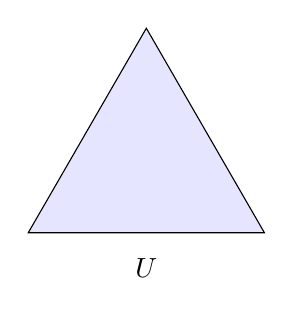
\begin{tikzpicture}[scale=3]

% Big equilateral triangle U
\coordinate (A) at (0,0);
\coordinate (B) at (1,0);
\coordinate (C) at (0.5,{sqrt(3)/2});

\fill[blue!10] (A)--(B)--(C)--cycle;
\draw (A)--(B)--(C)--cycle;
\node at (0.5,-0.15) {$U$};
\end{tikzpicture}
\end{center}
\end{minipage}
\begin{minipage}{0.45\textwidth}
\begin{center}
    
    \begin{tikzpicture}[scale=3]
% Similitude S1: scale by 1/3
\begin{scope}
  \fill[red!30] (0,0)--(1/3,0)--(0.5/3, {sqrt(3)/6})--cycle;
  \draw (A)--(B)--(C)--cycle;
\end{scope}

\node at (0.15,-0.12) {$S_1(U)$};

% Similitude S2: scale 1/3, rotate 60, shift
\begin{scope}
  \fill[green!20] (1/3,0)--(0.5/3, {sqrt(3)/6}) -- (1.5/3, {sqrt(3)/6}) -- cycle;
\end{scope}


% Similitude S3: scale 1/3, rotate -60, shift
\begin{scope}
  \fill[orange!30] (2.5/3,{sqrt(3)/6})--(1.5/3, {sqrt(3)/6})--(2/3,0)--cycle;
\end{scope}
\node at (0.66,0.25) {$S_3(U)$};

\node at (0.33,0.25) {$S_2(U)$};
\begin{scope}
  \fill[purple!30] (2/3,0)--(1,0)--(2.5/3,{sqrt(3)/6})--cycle;
\end{scope}
\node at (0.85,-0.12) {$S_4(U)$};

\end{tikzpicture}

\end{center}
\end{minipage}
~\\~\\
The coloured triangles show the similitude images on the open triangle (with the borders not included). These do not overlap, and are contained in the original open set, as required. By Theorem~\ref{thm:haus_similar_connection}, $\dim _HK = \dim _S \{S_1,S_2,S_3,S_4\} =:d$ such that
\[\frac{4}{3^d} = 1 \iff d = \frac{\ln 4}{ \ln 3}\] We have shown above that $S'$ is a similitude, and thus a bi-lipschitz map. So rotations and translations both preserve the Hausdorff dimension. So, by the countable stability property (from Theorem~\ref{thm:dimension}) of Hausdorff dimensions,
\[\dim_H S = \max \left \{\dim _H \left (K\left [ \frac{\pi}{3}\right ] \right ), \dim _H \left (K\left [ -\frac{\pi}{3}\right ]  + \left (\frac{1}{2}, \frac{\sqrt{3}}{2} \right )\right ), \dim _H \left (K\left [ \pi\right ] + (1,0) \right ) \right \} = \dim _H K = \frac{\ln 4}{\ln 3}\]

\subsection{Further Properties}
We will be considering the Koch Snowflake here, not the Koch Curve. The dimension being greater than one means that, by Theorem~\ref{thm:why_dimension} \[
\mathcal{H}^1(\mathcal{S}) = \infty
\]
That is, the Koch Snowflake has infinite length. One can easily find the internal area, using that the side length of the added equilateral triangles in iteration $n$ is $\ell _n = 3^{-n+1}=3\cdot 3^{-n}$ and thus has area $\frac{1}{2} \cdot \ell _n  \cdot \frac{\ell _n \sqrt{3}}{2}$. In iteration $n$, we have $s_n = 3 \cdot 4^{n-1} $ sides. Notice then in iteration $n$, we add $s_n$ new triangles (one for each side). So, we can solve for the area by the added triangles:
\[
A_1 = \frac{\sqrt{3}}{4}
\]
\[
\mathcal{A} = A_1 + \sum \limits _{n=2}^\infty (s_{n-1}) \cdot  \frac{\sqrt{3} \ell _n^2}{4} = \frac{2\sqrt{3}}{5}
\]

\newpage

\section{The Sierpinski Triangle}

To construct The Sierpinski Triangle, start with an equilateral triangle (with its area, say side length 1). Then, divide the triangle into 4 congruent triangles, and remove the middle triangle. Do this recursively, for each remaining triangle, subdivide it into 4 smaller congruent equilateral triangles and remove the middle one from each of these triangles.

\begin{center}
    \includegraphics[scale = 0.6]{assets/sierpinski_triangle.png}
\end{center}
We will denote the Sierpinski triangle as $\mathcal{T}$ and its iterations by $\mathcal{T}_n$. 
To rigorously desribe the triangle, we define it in terms of the similitudes:
\begin{align*}
    S_1(x,y) & = \frac{1}{2}(x,y) \\ S_2(x,y) & = \frac{1}{2}(x,y) + \left (\frac{1}{2}, 0 \right ) \\ S_3(x,y) & = \frac{1}{2}(x,y) + \left (\frac{1}{4},  \frac{\sqrt{3}}{4}\right )
\end{align*}
where $\mathcal{T}_0$ is the unit equilateral triangle, and \[
\mathcal{T}_{n+1} = \bigcup \limits _{i=1}^3 S_i(\mathcal{T}_n)
\]
We will define $\mathcal{T}$ as the unique invariant set under $\{S_1,S_2,S_3\}$. We can also show that:
\[
\mathcal{T}' := \bigcap \limits _{n \in \mathbb{N}_0} \mathcal{T}_n =\mathcal{T}
\]
Since \[
\mathcal{T}'=\bigcap \limits _{n\in \mathbb{N}_0} \mathcal{T}_n = \bigcap \limits _{n\in \mathbb{N}^+} \mathcal{T}_n  = \bigcap \limits _{n\in \mathbb{N}^+} \left [ \bigcup \limits _{i=1}^4 S_i(\mathcal{T}_{n-1})\right ] = \underbrace{\bigcup \limits _{i=1}^4 \left [ \bigcap \limits _{n \in \mathbb{N}^+} S_i(\mathcal{T}_{n-1})\right ] =\bigcup \limits _{i=1}^4 \left [ S_i \left (\bigcap \limits _{n \in \mathbb{N}^+} \mathcal{T}_{n-1} \right )\right ]}_{\text{Theorem}~\ref{thm:pres_sim}} = \bigcup \limits _{i=1}^4 S_i(\mathcal{T}')
\]
That is, $\mathcal{T} = \mathcal{T}'$ (so we can equally define it as the intersection of all these sets, and the unique invariant set)


\subsection{The Dimension of the Sierpinski Triangle}
We must show $\{S_1,S_2,S_3\}$ satisfy OSC. Just take $O$ to be the open unit equilateral triangle. Then, their images are:
\begin{itemize}
    \item[-] $S_1 (O)$ is the bottom left equilateral triangle in Iteration 1 (not including the boundary)
    \item[-] $S_2 (O)$ is the top equilateral triangle in Iteration 1 (not including the boundary)
    \item[-] $S_3 (O)$ is the bottom right equilateral triangle in Iteration 1 (not including the boundary)
\end{itemize}
These are disjoint and contained in the open set, as required. So \[
\dim_H(\mathcal{T}) = \dim _S \{S_1,S_2,S_3\} =:d
\] 
such that \[
\frac{3}{2^d} = 1 \iff d = \frac{\ln 3}{\ln 2}
\]
\subsection{Further Properties}
Since $\dim \mathcal{T} <2$, it follows $\mathcal{H}^2(\mathcal{T}) = 0$ (by Theorem~\ref{thm:why_dimension}) and the triangle has no area. However, we can calculate the perimeter recursively, with $P(\mathcal{T}_0) = 3$. The number of filled triangles in iteration $n$ is by $3^n$. Notice these all have the same size, with length $(\frac{1}{2})^n$. No two black triangles share a side, so the perimeter (denoted by $P$) is given by \[
P(\mathcal{T}_n) = 3^n \left[3 \cdot \frac{1}{2^n} \right ] = 3 \left ( \frac{3}{2}\right )^n \to \infty \text{ as } n \to \infty
\]
and perimeter is a measure so \[
P(\mathcal{T}) = P \left ( \bigcap \limits _{n \in \mathbb{N}_0} \mathcal{T}_n\right) = \lim \limits _{n \to \infty} P(\mathcal{T}_n)
\]
since $P(\mathcal{T}_0) = 3$ which is finite.
So the Sierpinski Triangle is a region with infinite perimeter but zero area.


\newpage

\section{The Sierpinski Carpet}
Begin with a square (let's say $[0,1] \times [0,1]$). The square is cut into 9 congruent subsquares and the central one is removed. We then recursively do this to all other squares that have area.

\begin{center}
    \includegraphics[scale = 0.3]{assets/sierpinski_carpet.png}
\end{center}
To define this rigorously, let $\mathcal{W}_0 = [0,1] \times [0,1]$. We define the reduction process using similitudes:
\begin{align*}
    S_1(x,y) & = \frac{1}{3}(x,y) + \left ( 0, 0\right )\\ 
    S_2(x,y) & = \frac{1}{3}(x,y) + \left ( \frac{1}{3}, 0\right ) \\ 
    S_3(x,y) & = \frac{1}{3}(x,y) + \left ( \frac{2}{3}, 0\right ) \\ 
    S_4(x,y) & = \frac{1}{3}(x,y) + \left ( 0, \frac{1}{3}\right )\\ 
    S_5(x,y) & = \frac{1}{3}(x,y) + \left ( \frac{2}{3}, \frac{1}{3}\right ) \\ 
    S_6(x,y) & = \frac{1}{3}(x,y) + \left ( 0, \frac{2}{3}\right )\\ 
    S_7(x,y) & = \frac{1}{3}(x,y) + \left ( \frac{1}{3}, \frac{2}{3}\right ) \\ 
    S_8(x,y) & = \frac{1}{3}(x,y) + \left ( \frac{2}{3}, \frac{2}{3}\right ) 
\end{align*}
For $n\ge 0$, define \[\mathcal{W}_{n+1} = \bigcup \limits _{i=1}^8 S_i(\mathcal{W}_n)\]
And let the Sierpinski Carpet $\mathcal{W}$ be the unique compact set invariant under $\{S_i\}_{i=1}^8$.
Again, we can indeed show that
\[
\mathcal{W}' := \bigcap \limits _{n \in \mathbb{N}_0}  \mathcal{W}_n= \mathcal{W}
\]
By noticing that
\[
\mathcal{W}'=\bigcap \limits _{n\in \mathbb{N}_0} \mathcal{W}_n = \bigcap \limits _{n\in \mathbb{N}^+} \mathcal{W}_n  = \bigcap \limits _{n\in \mathbb{N}^+} \left [ \bigcup \limits _{i=1}^8 S_i(\mathcal{W}_{n-1})\right ] = \underbrace{\bigcup \limits _{i=1}^8 \left [ \bigcap \limits _{n \in \mathbb{N}^+} S_i(\mathcal{W}_{n-1})\right ] =\bigcup \limits _{i=1}^4 \left [ S_i \left (\bigcap \limits _{n \in \mathbb{N}^+} \mathcal{W}_{n-1} \right )\right ]}_{\text{Theorem}~\ref{thm:pres_sim}} = \bigcup \limits _{i=1}^4 S_i(\mathcal{W}')
\]
So $\mathcal{W} = \mathcal{W}'$.

\subsection{The Dimension of the Sierpinski Carpet}
Let $O = (0,1) \times (0,1)$, then 
\begin{align*}
    S_1(O) & = \left (0, \frac{1}{3} \right) \times \left (0, \frac{1}{3} \right)\\ 
    S_2(O) & = \left (\frac{1}{3}, \frac{2}{3} \right) \times \left (0, \frac{1}{3} \right)\\ 
    S_3(O) & = \left (\frac{2}{3}, 1 \right) \times \left (0, \frac{1}{3} \right)\\ 
    S_4(O) & = \left (0, \frac{1}{3} \right) \times \left (\frac{1}{3}, \frac{2}{3} \right)\\ 
    S_5(O) & = \left (\frac{2}{3}, 1 \right) \times \left (\frac{1}{3}, \frac{2}{3} \right)\\ 
    S_6(O) & = \left (0, \frac{1}{3} \right) \times \left (\frac{2}{3}, 1 \right)\\ 
    S_7(O) & = \left (\frac{1}{3}, \frac{2}{3} \right) \times \left (\frac{2}{3}, 1 \right)\\ 
    S_8(O) & = \left (\frac{2}{3}, 1 \right) \times \left (\frac{2}{3}, 1 \right)
\end{align*}
These are disjoint and contained in $O$, so $\{S_i\}_{i=1}^8$ satisfies the OSC. Thus, by Theorem~\ref{thm:haus_similar_connection} \[
\dim _H \mathcal{W} = \dim _S \{S_i\}_{i=1}^8 =:d
\]
such that \[\frac{8}{3^d} = 1 \iff d = \frac{\ln 8}{\ln 3}\]
By Theorem~\ref{thm:why_dimension}, $\mathcal{H}^2(\mathcal{W}) = 0$, so the Sierpinski Carpet has no area.

\subsection{Sierpinski Carpet Relatives}
Start with a square rotated by $\frac{\pi}{4}$ $( = 45 ^\circ)$, and just like the Sierpinski Carpet, divide this into 9 smaller congruent squares. If the middle square is removed and the construction is iterated on the remaining squares, the result is the Sierpinski Carpet, but rotated 45°. We will introduce an orientation onto each of these smaller congruent squares. We will use arrows, up ($0$ radians rotated anticlockwise), down ($\pi$ radians), left ($\frac{\pi}{2}$ radians), and right $\frac{3\pi}{2}$ radians) to represent orientation. For example, if my orientation is left and my recursive process is to remove the top middle square, in that new orientation we are removing the left middle square. Let's look at a few examples
\begin{center}
    \includegraphics[scale = 0.4]{assets/up_middle.png}
\end{center}
This is the standard rotated Sierpinski Carpet
\begin{center}
    \includegraphics[scale = 0.4]{assets/up_top.png}
\end{center}
This is the rotated Sierpinski Carpet removing the top square
\begin{center}
    \includegraphics[scale = 0.4]{assets/up_lr.png}
\end{center}
This is the rotated Sierpinski Carpet, removing the top square but the left, right and middle squares are rotated
~\\~\\ We can look at the dimensions of such constructions. Suppose we remove $m$ squares, $1 \le m \le 7$ (as removing $8$ squares results in the unique invariant set being a point). Then we have $9-m$ similitudes (each of which could have some rotation, but as we have seen in the Koch Curve, rotations do not affect whether it is a similitude or not, just the scaling factor) and each similitude has contraction ratio $\frac{1}{3}$. Then we can use the open interior of our original square as our open set to get our similitudes satisfy the Open Set Condition, and so, if $\mathcal{F}$ represents our modified Sierpinski Carpet, by Theorem~\ref{thm:haus_similar_connection}, \[
\dim _H \mathcal{F} = d \text{ such that } (9-m) \left ( \frac{1}{3} \right)^d = 1 \iff d = \frac{\ln (9-m)}{\ln 3}
\]
There are $9 \choose m$ ways to remove $m$ squares, and any of the remaining $9-m$ squares can be 4 orientations. This gives
\[
\sum \limits _{m=1}^{7} {9 \choose m} 4^{9-m} = 1690944
\]
different fractals that form with this interpretation (some fractals are the ``same'' over some line of symmetry).~\\

\begin{center}
\noindent\fbox{%
    We can view the Sierpinski triangle as a generalization of the Cantor Set in 2 dimensions.
}
\end{center}


\newpage

\section{Pythagoras' Tree}

Chapters 6-9 introduced fractals that are self-similar and thus we could use the similarity dimension to classify their Hausdorff dimension. It will not always be the case that our fractals will be self-similar, represented by this next fractal. Instead, we must observe properties about our fractal and use the Hausdorff measure directly. The \textit{Pythagoras' tree} is a fractal constructed entirely from squares. It is named after the Pythagorean theorem, since each step in its construction involves a right-angled triangle.

\begin{enumerate}
    \item Begin with a unit square (let's say the bottom left corner is (0,0)). This is the root of the tree.
    \item On the top edge of this square, construct an 
    isosceles right triangle with the top edge as its hypotenuse. 
    \item On each of the two equal sides of the triangle, construct a new square outward. These two squares are the ``branches'' growing from the root square.
    \item Repeat the process recursively. On the top side of every newly added square, build a right triangle. On this triangle, place further squares. At each step, the squares become smaller, and the structure begins to resemble a branching tree.

    \item Mathematically, we will let $\mathcal{P}_n$ be the $n$-th iteration and the Pythagoras' Tree be \[
    \mathcal{P}= \bigcup \limits _{n \in \mathbb{N}_0} \mathcal{P}_n
    \]
\end{enumerate}

\begin{minipage}{0.45\textwidth}
    \begin{center}
        \includegraphics[scale = 0.4]{assets/p_tree_one.png}
    \end{center}
\end{minipage}
\begin{minipage}{0.55\textwidth}
    \begin{center}
        \includegraphics[scale = 0.35]{assets/p_tree_two.png}
    \end{center}
\end{minipage}
~\\
\subsection{The Dimension of the Pythagoras' Tree}
We do not get a contraction for the identity map representing the original part of the iteration we are building onto, so we cannot use self-similarity. Instead, notice the length of the squares added in iteration $n$ have side length $(\sqrt{2})^{-n}$. Then, for any $(x,y) \in \mathcal{T}$, \[
-\sum \limits _{n=1}^{\infty} (\sqrt{2})^{-n} \le x,y \le 1 + \sum \limits _{n=1} ^{\infty} (\sqrt{2})^{-n}
\]That is,
\[
-\frac{1/\sqrt{2}}{1-1/\sqrt{2}} \le x,y \le 1+ \frac{1/\sqrt{2}}{1-1/\sqrt{2}} \iff -1-\sqrt{2} \le x,y \le 2+\sqrt{2}
\]
So, since the unit square $[0,1] \times [0,1]$ is contained in every $\mathcal{P}_n$ and thus $\mathcal{T}$, we have that \[
[0,1] \times [0,1] \subseteq \mathcal{T} \subseteq \left [-1-\sqrt{2}, 2 + \sqrt{2} \right ] \times \left [-1-\sqrt{2}, 2 + \sqrt{2} \right ]
\]
And $\mathcal{H}^2 \left ([0,1] \times [0,1] \right ) = (\alpha (2))^{-1}, \mathcal{H}^2 \left ( \left [-1-\sqrt{2}, 2+\sqrt{2} \right ] \times \left [-1-\sqrt{2}, 2+\sqrt{2} \right ] \right ) = (\alpha (2))^{-1} (3+2\sqrt{2})^2 $ (Theorem~\ref{thm:lebesgue_haus}) ~\\So $0< \mathcal{H}^2(\mathcal{T}) < \infty $ and finally, by the definition of the Hausdorff dimension and Theorem~\ref{thm:why_dimension}, $\dim _H\mathcal{T} = 2$
\newpage

\section{A Cantor-Type Set}
We will now introduce a set whose dimension is positive (in fact, any positive number between 0 and 1), but measure is 0. For this, we define the modified Cantor Set, with contraction ratio $r \in \left (0,\frac{1}{2} \right)$, where we remove the middle $1-2r$ interval (we looked at the middle third Cantor set). Then a contraction ratio of $r$ means that the dimension of the Cantor Set is the solution to \[
2r^d = 1 \iff r^d = \frac{1}{2} \iff d = \frac{-\ln 2}{\ln r}
\] (This Cantor set is defined by similitudes $S_1 (x) = rx$ and $S_2 (x) = rx + (1-r)$)
~\\Now fix $0<s<1$. Choose an increasing, positive sequence $s_n \uparrow  s$ where $s_n \ne s$. For each $n$, we build a modified Cantor set, denoted by $C_n$, where our contraction ratio is now $r_n = 2^{-1/s_n} $. Notice that $0 < s_n < 1$ so $0 < r_n < \frac{1}{2}$, and this Cantor set is well-defined. Then each of these Cantor sets have Hausdorff dimension \[
\frac{-\ln 2}{\ln \left ( 2^{-1/s_n}\right )}=s_n
\]
Finally set
\[C:=\bigcup_{n=1}^\infty C_n.
\]
Then each $C_n$ has Hausdorff dimension $\dim_H C_n=s_n$. So, by Theorem~\ref{thm:dimension}\textcolor{blue}{.2}
\[\dim_H\bigg(\bigcup_{n=1}^\infty C_n\bigg)=\sup_{n\in \mathbb{N}^+}\dim_H C_n=\sup_{n\in \mathbb{N}^+} s_n=s.
\]
Hence $\dim_H C=s$. Now, for any fixed $n \in \mathbb{N}^+$, since $s_n<s$, by Theorem~\ref{thm:why_dimension}, we have $\mathcal{H}^s(C_n)=0$. Therefore, by subadditivity,
\[\mathcal{H}^s(C)\le\sum_{n=1}^\infty\mathcal{H}^s(C_n)=0.
\]
So $\mathcal{H}^s(C)=0$, as required.~\\~\\
If we simply take $s=\tfrac12$ and set
\[s_n=\tfrac12-\frac{1}{n+2},\qquad r_n=2^{-1/s_n}.
\]
Then form the Cantor sets $C_n$ and set $C$, the argument above shows $\dim_H C=\tfrac12$ while $\mathcal{H}^{1/2}(C)=0$.

\newpage

\section{Appendix}
\subsection{Appendix A: The Isodiametric Inequality}
To prove the Isodiametric Inequality, we turn to geometric methods, in particular the technique of Steiner symmetrization. Steiner symmetrization is a geometric process that transforms a set into a more “symmetric” one, while preserving certain properties such as volume. Let $\Omega \subseteq \mathbb{R}^n$ be a bounded domain (open, connected set with nonempty interior) with piecewise $C^1$ boundary. Let $L\subseteq \mathbb{R}^n$ be a hyperplane through the origin. Rotate the space such that $L$ is the $x_n = 0$ hyperplane. For each $\mathbf{x} \in L$, let the perpendicular line through $\mathbf{x}$ be \[
G_\mathbf{x} = \{\mathbf{x} + y \mathbf{e}_n: y \in \mathbb{R}^n\} 
\] the line orthogonal to $L$ that passes through $\mathbf{x}$, where $\mathbf{e}_n$ is the standard basis vector with $1$ in the $n$-th position. Let $m_\mathbf{x} = \mathcal{H}^1(\Omega \cap G_\mathbf{x})$ be the measure of the slice of $\Omega$ along $\Omega \cap G_\mathbf{x}$. We replace each slice $\Omega \cap G_\mathbf{x}$ by the centred interval on the same line having the same measure $m_\mathbf{x}$. The Steiner Symmetrization is then defined \[
S_L(\Omega ) = \left \{\mathbf{x} + y \mathbf{e}_n: \mathbf{x} + z\mathbf{e}_n \in \Omega \text{ for some } z \text{ and } -\frac{1}{2}m_\mathbf{x} \le y \le \frac{1}{2} m _\mathbf{x} \right \}
\]
where the role of $z$ is to detect whether the vertical line at horizontal position $x$ intersects $\Omega$.
The intuition behind this is at every ``base point" $\mathbf{x} \in L$ we take a vertical segment of measure $m_\mathbf{x}$, but we centre it on the hyperplane $L$ (i.e., it is symmetric with respect to $L$). All horizontal information is left untouched; only the placement along the normal direction $\mathbf{e}_n$ is altered. Let $\Pi : \mathbb{R}^n \to L$ be the orthogonal projection. That is, the map $\Pi (x_1,...,x_n) = (x_1,x_2,...,x_{n-1},0)$). 


\begin{center}
    \includegraphics[scale = 0.7]{assets/steiner.png}
\end{center}

\newpage

\begin{thm}\label{thm:steiner-vol}{\textbf{Steiner Symmetrization Preserves Volume}}
\end{thm}
\begin{proof}
    Let $\omega = \Pi (\Omega )$ be the projection in $L$. Since \[
    \Omega  = \{(\mathbf{x}, y): \mathbf{x} \in L, y \in \Omega \cap G_{\mathbf{x}}\}
    \]From Tonelli's Theorem we get
    \begin{align*}
        \lambda_n(\Omega ) & = \int _L \int _{\Omega \cap G_\mathbf{x}}1d\lambda _1 d\lambda _{n-1}\\ & = \int _{\omega } \left ( \int _{G_\mathbf{x} \cap \Omega }dx_n \right ) dx_1dx_2...dx_{n-1} \\ & = \int _{ \omega } m_{(x_1,...,x_{n-1},0)}dx_1dx_2...dx_{n-1} \\ & = \int _{\omega } \left ( \int _{ G_\mathbf{x} \cap S_L(\Omega)} dx_n\right )dx_1dx_2...dx_{n-1} \\ & = \lambda_n(S_L(\Omega ))
    \end{align*}
\end{proof}

\begin{thm}\label{thm:steiner-diam} \textbf{Steiner Symmetrization Reduces Diameter:}~\\
For any bounded set $\Omega \subset \mathbb{R}^n$, the Steiner symmetrization
satisfies
\[
\mathrm{diam}(S_L(\Omega)) \leq \mathrm{diam}(\Omega).
\]
\end{thm}

\begin{proof}~\\
    \begin{center}
    \includegraphics[scale = 0.5]{assets/iso.png}
\end{center}
Let $L$ be the hyperplane along which we symmetrize, and let $G_\mathbf{x}$ denote the line
orthogonal to $L$ through $\mathbf{x} \in L$.  
For each $\mathbf{x} \in L$, the slice $G_\mathbf{x} \cap \Omega$ is an interval $[a,b]$ of
length $m_\mathbf{x} = b-a$.  
After symmetrization, this slice becomes the interval 
$\left[-\tfrac{m_\mathbf{x}}{2}, \tfrac{m_\mathbf{x}}{2}\right]$. Now take two points $(\mathbf{x},z),(\mathbf{y},w) \in S_L(\Omega)$ with $\mathbf{x},\mathbf{y} \in L$.  
We want to show
\[
d\big((\mathbf{x},z),(\mathbf{x},w)\big) \leq \mathrm{diam}(\Omega).
\]
We have a two cases: ~\\
\textbf{Case 1: Both points come from the same slice.}  
Suppose $\mathbf{x}=\mathbf{y}$.  
Then the maximal vertical distance after symmetrization is
\[
|z-w| \leq m_\mathbf{x}.
\]
But in the original set $\Omega$, the same vertical slice had length $m_\mathbf{x}$, so 
\[
d\big((\mathbf{x},z),(\mathbf{y},w)\big) \leq m _{\mathbf{x}} \leq \mathrm{diam}(\Omega).
\]
\textbf{Case 2: Points from different slices.}  
Suppose $\mathbf{x} \neq \mathbf{y}$.  
Let
\[
a = \min(G_\mathbf{x} \cap \Omega), \quad b = \max(G_\mathbf{x} \cap \Omega), \quad
c = \min(G_\mathbf{y} \cap \Omega), \quad d = \max(G_\mathbf{y} \cap \Omega).
\]
Thus the vertical slices are $[a,b]$ and $[c,d]$. Before symmetrization, in the original set, the longest possible vertical difference between the two
slices is $\max\{|b-c|,|d-a|\}$.  
The corresponding squared distance is
\[
\delta^2 = (b-c)^2 + \|\mathbf{x}-\mathbf{y}\|^2
\quad \text{or} \quad
\delta^2 = (d-a)^2 + \|\mathbf{x}-\mathbf{y}\|^2.
\] 
After symmetrization, the slices become
\[
\Big[-\tfrac{m_\mathbf{x}}{2}, \tfrac{m_\mathbf{x}}{2}\Big]
\quad \text{and} \quad
\Big[-\tfrac{m_\mathbf{y}}{2}, \tfrac{m_\mathbf{y}}{2}\Big],
\]
where $m_\mathbf{x} = b-a$ and $m_\mathbf{y} = d-c$.  
Thus the maximal vertical separation is
\[
\frac{m_\mathbf{x}}{2} + \frac{m_\mathbf{y}}{2}.
\]
So the squared distance is
\[
\tilde{\delta}^2 = \left(\tfrac{m_\mathbf{x}+m_\mathbf{y}}{2}\right)^2 + \|\mathbf{x}-\mathbf{y}\|^2.
\]
Since $\max\{|b-c|,|d-a|\} \geq \tfrac{m_\mathbf{x}+m_\mathbf{y}}{2}$, we have
\[
d((\mathbf{x}, z), (\mathbf{y}, w))^2 \le \tilde{\delta}^2 \leq \delta^2 \le \diam (\Omega)
\] 
So
\[
\mathrm{diam}(S_L(\Omega)) \leq \mathrm{diam}(\Omega).
\]
    
\end{proof}

\newpage

~\\Now we are ready to prove the isodiametric inequality

\begin{thm}{\textbf{Isodiametric Inequality}} ~\\
    Let $K \subseteq \mathbb{R}^n$ be a compact domain. Then the volume satisfies 
    \[
    \lambda_n(K) \le \frac{\lambda_n(B(\mathbf{0}; 1)) \diam (K )^n}{2^n}
    \]

\end{thm}

\begin{proof}
    Note that $K$ being compact means it has finite volume. Choose a family of $n$ mutually perpendicular hyperplanes $\{L_i\}$ (e.g., the coordinate hyperplanes) and perform Steiner symmetrisations
    \[
    K_n = S_{L_n} \circ S_{L_{n-1}} \circ \dots \circ S_{L_1}(K)
    \]
    These $n$ symmetrisations result in a shape that is symmetric with respect to every coordinate hyperplane, thus is centrally symmetric. After symmetrization, each slice parallel to a coordinate axis is replaced by a centered interval about 0. So any line through the origin parallel to a coordinate axis is an interval symmetric about 0. This idea gives us that we have a star-shaped $K_n$ that is a centrally symmetric body. Since, for every $\mathbf{x} \in K_n$, the Steiner symmetrizations reduce diameter (Theorem \ref{thm:steiner-diam}), \[d(\mathbf{x}, -\mathbf{x}) \le \diam (K_n) \le \diam (K)\]it follows that 
    \[K_n \subseteq \overline{B} \left (\mathbf{0}; \frac{1}{2} \diam (K ) \right )\]
    and then, since the Steiner symmetrization preserves volume (Theorem \ref{thm:steiner-vol}) \[
    \lambda _n (K) = \lambda _n(K_n) \le \lambda _n \left ( \overline{B} \left (\mathbf{0}, \frac{1}{2} \diam (K) \right) \right ) = \lambda _n(B(\mathbf{0}; 1)) \left ( \frac{1}{2} \diam (K) \right)^n
    \]
\end{proof}

\newpage


\subsection{Appendix B: Connection between the Hausdorff and Lebesgue Measure}
Now to prove the relationship between the Hausdorff measure to the Lebesgue measure, we need the following theorem (whose proof is in Appendix A), and some background knowledge:

\begin{thm} \label{thm:isodiametric}
    The isodiametric inequality: For $A \subseteq \mathbb{R}^n$, $\lambda_n(A) \le \alpha (n) \diam (A)^n$
\end{thm}

\subsubsection*{An Excursion into Measure Theory}

\begin{thm} \label{thm:cubes_approx}
    For any set $A \subseteq \mathbb{R}^n$, $\varepsilon>0$ and $\Delta >0$ with $\lambda _n(A)<\infty$, we have the following:
    \begin{enumerate}
        \item There is a family of open cubes $\{Q_m\}_{m \in \mathbb{N}}$ such that $Q_m \subseteq A$ and $\sum \limits _{m=1}^\infty\lambda_n(Q_m) > \lambda_n(A)-\varepsilon$ and $\diam (Q_m)\le \Delta$ \\ (approximating sets with cubes from below)
        \item There is a $\Delta$-covering of open cubes $\{Q_m\}_{m\in \mathbb{N}}$ such that $\sum \limits _{m=1}^\infty\lambda _n(Q_m) < \lambda _n(A)+\varepsilon$ 
        \\ (approximating sets with cubes from above)
    \end{enumerate}
    

\end{thm}

\begin{proof}
    Since $\lambda_n(A) < \infty$, for $\varepsilon>0$, there exists a countable collection of open rectangles $\{U_m\}_{m\in \mathbb{N}} = \left \{\prod \limits _{i=1}^n (a_{mi}, b_{mi})\right \}_{m\in \mathbb{N}}$ such that 
    \[A \subseteq \bigcup \limits _{m \in \mathbb{N}} U_m \text{ and } \sum \limits _{m\in \mathbb{N}} \text{vol}(U_m) \le \lambda_n(A) + \varepsilon/2\]
   For some $\delta >0$, consider open cubes of side length $\delta $, of the form:
        \[(\delta k_1, \delta (k_1+1)) \times \cdots \times (\delta k_n, \delta (k_n+1)) \text{ for integers }k_1, ..., k_n\in \mathbb{Z} \ \ \ \ (***)\]
    Denote the set of all such cubes, for a fixed $\delta$ by $\mathcal{Q}^\delta $


\begin{center}
\tdplotsetmaincoords{60}{120} % 3D viewing angle

\begin{tikzpicture}[tdplot_main_coords, scale=1.5]

  % bottom square
  \draw[red]  (2,0,0) -- (2,2,0) -- (0,2,0);
  % top square
  \draw[red] (0,0,2) -- (2,0,2) -- (2,2,2) -- (0,2,2) -- cycle;
  % vertical edges
  \foreach \x/\y in {2/0, 2/2, 0/2} {
    \draw[red] (\x,\y,0) -- (\x,\y,2);
  }

  \draw[red] (1, 2, 0) -- (1, 2, 2) -- (1, 0, 2);
  \draw[red] (2, 1, 0) -- (2,1,2) -- (0, 1, 2);
  \draw[red] (2, 0, 1) -- (2, 2, 1) -- (0, 2, 1);

  % axes
  \draw[->, thick] (2,0,0) -- (2.7,0,0) node[anchor=north east]{$x$};
  \draw[->, thick] (0,2,0) -- (0,2.7,0) node[anchor=north west]{$y$};
  \draw[->, thick] (0,0,2) -- (0,0,2.7) node[anchor=south]{$z$};
\end{tikzpicture}
\end{center} ~\\
        Let $\mathcal{Q}_m ^\delta  = \left \{Q \in \mathcal{Q}^\delta : Q \subseteq U_m\right \}$ (all cubes of side length $\delta$ that are inside $U_m$) and $U_m ^\delta := \bigcup \mathcal{Q}_m^\delta$. Clearly $U_m^\delta \subseteq U_m$ and $U_m^\delta$ is a union of cubes. Moreover, for any $\mathbf{u_m} =(u_{m1}, ..., u_{mn}) \in U_m$ and
        \[ \delta = \min_{1\le i\le n} \{ \min \{u_{mi} - a_{mi}, b_{mi} - u_{mi}\}\} > 0 \text{  since } u_{mi} \ne a_{mi} \text{ and } u_{mi}\ne b_{mi}\]
        (the smallest distance to a border in the rectangle). Then take cube 
        \[C = \left \{(x_1,\dots, x_n) \in \mathbb{R}^n:u_{mi} - \frac{\delta }{2} <x_i<u_{mi} +\frac{\delta}{2}\right \} \subseteq U_m \]
        We are not guaranteed that the boundaries align with the form required. But since each side is length $\delta$, we can find a $\frac{\delta}{2}$ cube inside $C$ (otherwise, if one side length is contained in 2 $\frac{\delta}{2}$ cubes, its length must exceed $\delta$). Denote this cube by $C_{\delta /2}$. Since $\mathbf{u_m}$ is the center of $C$, it is in $C_{\delta/2}$ and we know $C_{\delta/2 } \in \mathcal{Q}_m^{\delta/2}$.

        \begin{figure}[h]
        \begin{center}
            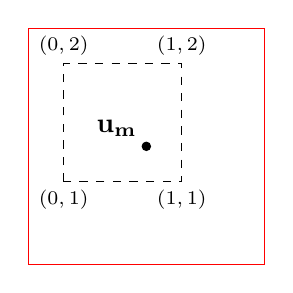
\begin{tikzpicture}[scale=1.5]
            % square centered
            \draw[red] (-0.3,0.3) -- (-0.3,2.3) -- (2-0.3,2.3) -- (2-0.3,0.3) -- cycle;

            \draw[fill=black] (0.7,1.3) circle (1pt);
            \node[above left] at (0.7,1.3) {$\mathbf{u_m}$};

            \draw[black, dashed] (0,1) -- (0,2) -- (1,2) -- (1,1) -- cycle;

\scriptsize{
            \node[below] at (0,1) {$(0,1)$};
            \node[below] at (1,1) {$(1,1)$};
            \node[above] at (0,2) {$(0,2)$};
            \node[above] at (1,2) {$(1,2)$};
            }
            \end{tikzpicture}
        \end{center}
        \caption{A square, length 2, centred at (0.7, 1.3) showing a containing square for $\delta =2$}
        \end{figure}
    
        
        So $\bigcup \limits _{\delta >0} U_m^\delta = U_m$. Also, all these sets are Borel sets (as rectangles), so \[
        |\lambda _n(U_m^\delta) - \lambda _n(U_m)|= |\lambda_n(U_m^\delta) - \lambda _n((U_m\setminus U_m ^\delta ) \cup U_m^\delta )| = \lambda_n(U_m \setminus U_m^\delta )
        \]
        But since $U_m^\delta$ is the maximal area of these $\delta$-squares contained in $U_m$, and that we have a smallest and largest integers $k_{11}, k_{12}, ..., k_{n1}, k_{n2}$ such that 
        \[(\delta k_{11}, \delta k_{12}) \times ...\times (\delta k_{n1}, \delta k_{n2}) \subseteq U_m \]  and replacing any $k_{i1}$ with $k_{i1}-1$, or $k_{i2}$ with $k_{i2}+1$, then it is no longer a subset. 
        
        \begin{figure}[h]
        \begin{center}
            \begin{tikzpicture}[scale=1.5]

            \draw[red] (-0.5, -0.5) -- (3.5, -0.5) -- (3.5, 2.5) -- (-0.5, 2.5) -- cycle;

             \foreach \x/\y in {0/0, 0/1, 1/0, 1/1, 2/0, 2/1}
            \draw[black, dashed] (\x, \y) -- (\x+1, \y) -- (\x + 1, \y + 1) -- (\x, \y + 1) -- cycle;
            \end{tikzpicture}
        \end{center}
        \caption{A rectangle, with its contained $\delta$ squares for $\delta  = 1$}
        \end{figure}
        
        
        
        
        
        
        Then $U_m \setminus U_m ^\delta \subseteq (\delta (k_{11}-1), \delta (k_{12} + 1)) \times  \dots \times  (\delta (k_{n1}-1), \delta (k_{n2} + 1)) \setminus (\delta k_{11}, \delta k_{12}) \times \dots \times (\delta k_{n1}, \delta k_{n2})$ and thus
        \[
        \lambda_n(U_j \setminus U_j^\delta ) \le \delta  \sum \limits _{i=1}^n (2+k_{12}-k_{11}) - \delta \sum \limits _{i=1}^n (k_{12} - k_{11}) = 2n\delta \to 0 \text{ as } \delta \to 0
        \]
    ~\\ 
        So $\lambda _n(U_m^\delta ) \to \lambda _n(U_m)$. Let $\delta^L _m$ be delta small enough such that $\lambda _n(U_m^{\delta_m^L})<\lambda_n(U_m) - \frac{\varepsilon}{2} 2^{-m}$ and $\delta _m \le \Delta$. \\ ~\\
        If we let $I_ {m} ^\delta= (\delta (k_{11}-1), \delta (k_{12} + 1)) \times  \dots \times  \delta (k_{n1}-1), \delta (k_{n2} + 1))$, then we approach $U_m$ from outside with $I^\delta _m \setminus U_m \subseteq (\delta (k_{11}-1), \delta (k_{12} + 1)) \times \dots \times (\delta (k_{n1}-1), \delta (k_{n2} + 1)) \setminus (\delta k_{11}, \delta k_{12}) \times \dots \times (\delta k_{n1}, \delta k_{n2})$ (the same as above) and so
        $\lambda _n(I_m^\delta) \to \lambda_n(U_m)$. Let $\delta^U _m$ be delta small enough such that $\lambda_n(I_m^{\delta^U_m})<\lambda_n(U_m) + \frac{\varepsilon}{2} 2^{-m}$ and $\delta^U _m \le \Delta$. \\ Then we let $I_m^{\delta_m^U}$ be described as above, and my family of cubes is the family of all cubes for all $m\in \mathbb{N}^+ $, denoted $\{Q_m\}_{m \in \mathbb{N}}$, then clearly $\diam (Q_m)\le \delta_m^U \le \Delta$, and 
        
        \[
        \sum \limits _{m=1}^\infty \lambda_n(Q_m)<\sum \limits _{m=1}^\infty(\lambda_n (U_m) + \frac{\varepsilon}{2}2^{-m}) = \sum \limits _{m=1}^\infty\lambda_n (U_m) + \varepsilon/2 \le \lambda_n(A) + \varepsilon 
        \]
        and using the cubes from $U_m^{\delta_m^L}$, labelled as $\{Q_m\}_{m\in \mathbb{N}}$, we get
        \[
        \sum \limits _{m=1}^\infty \lambda_n(Q_m)>\sum \limits _{m=1}^\infty(\lambda_n (U_m) - \frac{\varepsilon}{2}2^{-m}) = \sum \limits _{m=1}^\infty\lambda_n (U_m) - \varepsilon/2 \ge \lambda_n(A) - \varepsilon
        \]
        since $\lambda_n(A)$ is the infimum and clearly $\varepsilon/2 \le \varepsilon$

    
\end{proof}

\begin{thm} \label{thm:circumscribing_ball}
    For any $n$-dimensional cube $Q \subseteq \mathbb{R}^n$, there exists a ball $B$ such that $Q \subseteq B$ and their $n$-dimensional Lebesgue measures satisfy the inequality:
$$
\lambda_n(B) = c_n \lambda_n(Q)
$$
where the constant $c_n$ is the ratio of the volume of the minimal circumscribing ball to the volume of the cube, given by
$$
c_n = \frac{\pi^{n/2} n^{n/2}}{2^n \Gamma\left(\frac{n}{2}+1\right)}.
$$
\end{thm}


\begin{proof}
    We know $\lambda_n(Q) = r^n$ for cube side length $r$ with center $\mathbf{c}$. Then we can consider closed ball $\overline{B} \left(\mathbf{c}; \frac{\sqrt{n}}{2}r \right)$ (the circumscribing ball), then  \[\lambda_n(B) = \frac{\pi^{n/2}}{\Gamma(\frac{n}{2}+1)}\left(\frac{\sqrt{n}}{2}r\right)^n =\frac{\pi ^{n/2} n^{n/2}}{2^n \Gamma (\frac{n}{2}+1)}r^n = \frac{\pi ^{n/2} n^{n/2}}{2^n \Gamma (\frac{n}{2}+1)} \lambda_n(Q)\]
\end{proof}

\subsubsection*{An Excursion into Metric Spaces}

\begin{prop}
    Let $\mathcal{F}$ be a finite collection of open balls in $(X,d)$. Then there exists a subcollection $\mathcal{G} \subseteq \mathcal{F}$ of pairwise disjoint balls such that any ball $B(a;r) \in \mathcal{F}$ intersects a ball $B(a'; r') \in \mathcal{G}$ with $r' \ge r$
\end{prop}
\begin{proof}
    Suppose that $\mathcal{F} = \{B(a_i; r_i)\}_{i=1}^n$ with $r_1 \ge r_2 \ge ... \ge r_n$. We inductively define $\mathcal{G}$ as follows:
    $B(a_1; r_1) \in \mathcal{G}$, and for $2 \le k \le n$, $B(a_k;r_k) \in \mathcal{G} $ iff $B(a_k; r_k)$ is disjoint from every ball in \[
    \{B(a_1; r_1), B(a_2; r_2), ..., B(a_{k-1}; r_{k-1})\} \cap \mathcal{G}
    \]
    Now if $B(a_k;r_k) \notin \mathcal{G}$, then it intersects some $B(a_j;r_j) \in \mathcal{G}$ with $j < k$ and $r_j \ge r_k$ and we are done (since $B(a_k;r_k) \in \mathcal{G}$ is trivial)
\end{proof}
~\\ This has the following consequence:

\begin{thm}{\textbf{Vitali's Covering Lemma (finite case)}} ~\\
    Let $\mathcal{F}$ be a finite collection of open balls in $(X,d)$. Then there exists a subcollection $\mathcal{G} \subseteq \mathcal{F}$ of pairwise disjoint balls such that
    \[
    \bigcup \mathcal{F} \subseteq \bigcup \{B(a_i; 3r_i):B(a_i; r_i) \in \mathcal{G}\}
    \]
\end{thm}

\begin{proof}
    Let $\mathcal{G}$ be as in the previous proposition and take $B(a; r) \in \mathcal{F}$. Then there exists an open ball $B(a'; r')$ that intersects $B(a;r)$ with $r' \ge r$. Let $x \in B(a;r)$ and $y \in B(a;r) \cap B(a';r')$. Then 
    \[d(a',x) \le d(a', y) + d(y,a) + d(a, x) < r' + r + r \le 3r' \text{ so } B(a;r) \subseteq B(a', 3r')\]completing the proof.
\end{proof}

Note that the above results still hold if open balls are replaced by closed balls throughout.

~\\For an infinite collection of balls, we can no longer sort them by radius. However, the following weaker version still holds:

\begin{prop}
    Let $\mathcal{F}$ be any collection of open balls in $(X,d), $ each with radius at most $R < \infty$. Then there exists a subcollection $\mathcal{G} \subseteq \mathcal{F}$ of pairwise disjoint balls, such that any ball $B(a;r) \in \mathcal{F}$ intersects a ball $B(a',r') \in \mathcal{G}$ with $2r' > r$
\end{prop}

\begin{proof}
    Partition $\mathcal{F}$ into subcollections
    \[
    \mathcal{F}_n = \left \{B(a;r) \in \mathcal{F}:\frac{R}{2^n} \le r < \frac{R}{2^{n-1}} \right \}
    \]
    Inductively define subcollections $\mathcal{G}_n \subseteq \mathcal{F}_n$ as follows. Let $\mathcal{G}_1$ be a maximal subcollection of pairwise disjoint balls in $\mathcal{F}_1$. This exists by Zorn's lemma, by considering the collection of all subcollections of disjoint balls of $\mathcal{F}_1$, ordered under inclusion. Let $\{C_i\}_{i\in I}$ be any chain of subcollections of pairwise disjoint balls from $\mathcal{F}_1$. Then $C = \bigcup \limits _{i=1} ^ \infty C_i$ is an upper bound, because if $B_1,B_2 \in C$, then there exists $i,j \in I$ with $B_1 \in C_i$, $B_2 \in C_j$. Since the collection forms a chain, either $C_i \subseteq C_j$ or $C_j \subseteq C_i$. In either case, both balls belong to the same subcollection of pairwise disjoint balls, so they're disjoint.  \\ For $n > 1$, if $\mathcal{G}_k$ has been defined for all $1\le k < n$, let $\mathcal{G}_n$ be a maximal subcollection of pairwise disjoint balls in 
    \[
    \mathcal{H}_n = \left \{ B \in \mathcal{F}_n: \forall C \in \bigcup \limits _{k=1}^{n-1} \mathcal{G}_k, \ B \cap C = \emptyset \right \}
    \]
    (which exists by Zorn's lemma, and is all balls in $\mathcal{F}_n$ disjoint from all previously included balls). Let $\mathcal{G} = \bigcup \limits _{n=1} ^\infty \mathcal{G}_n$.
    \\ ~\\ Now for every $B \in \mathcal{F}_n$, we have one of the following:
    \begin{itemize}
        \item $B \in \mathcal{G}_n$;
        \item $B \in \mathcal{H}_n \setminus \mathcal{G}_n$ so $B$ intersects some ball in $\mathcal{G}_n$ (since $\mathcal{G}_n$ is maximal, so if it doesnt, $\mathcal{G}_n \cup \{B\}$ contradicts that); or
        \item $B \notin \mathcal{H}_n$, so $B$ intersects some ball in $\mathcal{G}_k$ for some $k < n$
    \end{itemize}
    In any case, $B$ intersects a ball in $\mathcal{G}$, more specifically, in $\mathcal{G}_k$ for some $k 
    \le n$ of radius $r'$ with
    \[
    2r' \ge 2 \frac{R}{2^k} \ge 2\frac{R}{2^n} = \frac{R}{2^{n-1}} > r
    \]
    as desired.
\end{proof}
Just as in the finite case, we can deduce a version of Vitali's covering lemma:

\begin{thm}{\textbf{Vitali's Covering Lemma (infinite case)}}\label{thm:vitali_inf}
    ~\\Let $\mathcal{F}$ be a collection of open balls in $(X,d)$, each with radius at most $R < \infty$. Then there exists a subcollection $\mathcal{G} \subseteq \mathcal{F}$ of pairwise disjoint balls, such that
    \[
    \bigcup \mathcal{F} \subseteq \bigcup \{B(a;5r): B(a;r) \in \mathcal{G}\}
    \]
\end{thm}

\begin{proof}
    Take $\mathcal{G}$ as in the previous proposition. For any $B(a;r) \in \mathcal{F}$, take $B(a', r') \in \mathcal{G}$ intersecting $B(a;r)$, and a point $x \in B(a;r) \cap B(a', r')$. Then for any $y \in B(a;r)$, \[
    d(a',y) \le d(a', x) + d(x,a) + d(a,y) <r' +r+r\le 5r'
    \]
    Hence $B(a,r) \subseteq B(a', 5r')$ which finishes the proof
\end{proof}

\subsubsection*{Vitali Covers}

\begin{defn}
    A ball $B(a;r)$ or $\overline{B}(a;r)$ in $\mathbb{R}^n$ is called \textit{nondegenerate} if it contains a point other than its centre $a$, or equivalently, if $r > 0$
\end{defn}

\begin{defn}
    Let $A \subseteq \mathbb{R}^n$. A collection $\mathcal{F}$ of nondegenerate closed balls in $\mathbb{R}^n$ is a Vitali cover of $A$ if for all $x\in A$ and $\delta >0$, there is a ball $B(a;r) \in \mathcal{F}$ such that $r < \delta$ and $x\in B(a;r)$. In other words, every point in $A$ is covered by an arbitrary small ball in $\mathcal{F}$
\end{defn}

\begin{thm}{\textbf{Vitali Covering Theorem}}~\\
    Let $A \subseteq \mathbb{R}^n$ be a set (not necessarily measurable), and $\mathcal{F}$ a Vitali cover of $A$. Then there exists a subcollection $\mathcal{G} \subseteq \mathcal{F}$ of pairwise disjoint balls such that \[
    \lambda _n \left ( A \setminus \bigcup \mathcal{G} \right ) = 0
    \]
    
\end{thm}

\begin{proof}
    Note that removing every ball of radius greater than 1, we still end up with a Vitali cover of $A$. Hence we may assume that the balls in $\mathcal{F}$ have radius at most 1. Take $\mathcal{G}$ as in the last proposition with closed balls. We claim that this $\mathcal{G}$ satisfies the required condition; to prove this, it suffices to show that $\left (A \setminus \bigcup \mathcal{G} \right ) \cap B(0;R)$ is $\lambda _n$-null for every $R>0$. \\ ~\\ 
    Fix $\varepsilon > 0$. Let $\mathcal{G}'$ be the subcollection of balls in $\mathcal{G}$ which intersect $B(0, R)$.
Note that balls in $\mathcal{G}'$ are all contained in $B(0, R + 2)$. To see this, take a ball $\overline{B}(a;r) \in \mathcal{G}'$ and let $y \in \overline{B}(a;r) \cap B(0;R)$ and $x \in \overline{B}(a;r)$. Then \[
d(x,0) \le d(x,y) + d(y,0) \le r+R < R+2
\]
so
\[
\sum_{\overline{B}(a,r) \in \mathcal{G}'} \lambda_n(\overline{B}(a, r)) \leq \lambda_n(B(0, R + 2)) < \infty.
\]
Hence there exists $\delta>0$ such that
\[
\sum_{\substack{\overline{B}(a,r) \in \mathcal{G}' \\ r < \delta}} \lambda(\overline{B}(a, r)) < \frac{\varepsilon}{5^n}.
\]

Also, note that balls in $\mathcal{G}'$ with radius at least $\delta$ have Lebesgue measure at least $\lambda(B(0, \delta)) > 0$; hence there are only finitely many such balls, so $K = \bigcup \limits _{{\substack{\overline{B}(a;r) \in \mathcal{G}' \\ r \ge \delta}}} \overline{B}(a;r)$ is a closed set (as a finite union of closed sets).

Since $\mathcal{G}$ is a Vitali cover, for any point $a \in (A \setminus \bigcup \mathcal{G}) \cap B(0, R)$ there exists a small enough ball $B_a \in \mathcal{G}$ such that:
\begin{itemize}
\item $a \in B_a$ % (so $B_a \in \mathcal{G}'$);
\item $B_a \subseteq B(0, R)$; and
\item $B_a \cap K = \emptyset$.
\end{itemize}
By the proposition, $B_a$ intersects some ball $C_a \in \mathcal{G}$; since $B_a \subseteq B(0, R)$, we have $C_a \in \mathcal{G}'$. However, since $B_a$ is disjoint from $K$, the radius of $C_a$ is less than $\delta$.

Finally, we have $B_a \subseteq 5C_a$, so
\begin{align*}
\lambda_n\left((A \setminus \bigcup \mathcal{G}) \cap B(0, R)\right) &\leq \sum_{a \in (A \setminus \bigcup \mathcal{G}) \cap B(0, R)} \lambda_n(B_a) \\
&\leq \sum_{a \in (A \setminus \bigcup \mathcal{G}) \cap B(0, R)} \lambda_n(5C_a) \\
&\leq 5^n \sum_{\overline{B}(a,r) \in \mathcal{G}', r < \delta} \lambda_n(\overline{B}(a, r)) < \varepsilon.
\end{align*}

Hence $\lambda\left((A \setminus \bigcup \mathcal{G}) \cap B(0, R)\right) = 0$, as desired. $\square$
\end{proof}
From this, we deduce a useful proposition.
\begin{prop} \label{prop:ball_cover}
    Let $Q$ be an $n$-dimensional cube. Then there exists a countable collection $\{B_i\}_{i =1}^\infty$ of pairwise disjoint closed balls such that
    \[
\lambda_n\left(Q \setminus \bigcup_{i=1}^{\infty} B_i\right) = 0.
\]
\end{prop}

\begin{proof}
    We first create a Vitali cover of $Q$. Define the collection
    \[
\mathcal{F} = \left\{\overline{B}\left(x, \frac{1}{k}\right) : x \in Q, k \in \mathbb{N}\right\}.
\]
Let $x \in Q$ and $\delta > 0$. Take $k \in \mathbb{N}$ large enough such that $\frac{1}{k} < \delta$. Then clearly ball $\overline{B}\left (x;\frac{1}{k} \right ) \in \mathcal{F}$ contains $x$ with radius less than $\delta$, so it is a Vitali cover of $Q$. By Vitali's Covering Theorem, there exists a subcollection $\mathcal{G} \subseteq \mathcal{F}$ of pairwise disjoint closed balls such that
\[
\lambda_n\left(Q \setminus \bigcup \mathcal{G}\right) = 0.
\]
Take any $q \in Q$ and let $r$ be the side length of $Q$. Then each ball in $\mathcal{F}$ is in ball $\overline{B}(q; r+2)$. So \[
\sum \limits _{B\in \mathcal{G}} \lambda _n(B) \le \lambda _n(\overline{B}(q;r+2)) < \infty
\]
And, since $\lambda _n(B) > 0$, it follows we have at most countably many balls. Rigorously, let $D_{\varepsilon} = \{B \in \mathcal{G}: \lambda_n(B) > \varepsilon\}$. Then each $D_{1/n}$ must be finite countable (otherwise we contradict that $\lambda _n(\overline{B}(q; r+2))$ is finite) and then $\mathcal{G} = \bigcup \limits _{n \in \mathbb{N}} D_{1/n}$ is countable.
\end{proof}






\begin{thm}
    We can relate the Hausdorff measure to the Lebesgue measure: 
    \begin{enumerate}
        \item $\mathcal{H}^0$ is the counting measure on measure space $(\mathbb{R}^n, \mathcal{P}(\mathbb{R}^n))$ (not just for $\mathcal{M}(\mathcal{H}^0)$)
        \item $\mathcal{H}^1_N=\mathcal{H}^1 = \lambda_1$ on $\mathbb{R}$ (as outer measures)
        \item $\mathcal{H}^n_N = \lambda_n$ on $\mathbb{R}^n$ for $n \in \mathbb{N}$ (as outer measures)
    \end{enumerate}
\end{thm}

\begin{proof} 
Since we can cover $\mathbb{R}^n$ with any countable $\delta$-covering, using closed cubes, any set has a covering as well.
    \begin{enumerate}
        \item We know $\mathcal{H}^0(\emptyset) = 0$. If $A \subseteq \mathbb{R}^n$ with $|A|=m \in 
        \mathbb{N}$, then $A = \{\mathbf{a_1}, \mathbf{a_2}, ..., \mathbf{a_m}\}$ 
        
        
        and we can cover $A$ with the family $\{\{\mathbf{a_n}\}\}_{n=1}^m$ and $\diam \{\mathbf{a_n}\} = 0$ and so $(\diam \{\mathbf{a_n}\})^0 = 1$ for each $n=1,2,...,m$. Thus $\mathcal{H}^0(A) \le \sum \limits _{i=1}^m 1 = m$. On the other hand, set $0<\delta < \min \{|\mathbf{a_i} - \mathbf{a_j}|: i\ne j, 1\le i,j\le m\}$ if we cover $A$ with a $\delta$-covering $\{E_n\}_{n\in \mathbb{N}}$, then clearly each $|E_n| = 1$ and for every $1\le i\le m$, we have there is some $1\le j\le m$ such that $\mathbf{a_i} \in E_j$, there must be at least $m$ non-empty sets. So $\sum \limits _{i=1}^\infty \diam (E_i)^0 \ge \sum \limits _{i=1}^m 1 = m$. So $\mathcal{H}^0(A) = m$. Now if $|A| = \infty$, then for each $n \in 
        \mathbb{N}$, let $A_n = \{\mathbf{a_n}_1, \mathbf{a_n}_2, ..., \mathbf{a_n}_n\} \subseteq A$. Then \\ $\mathcal{H}^0(A_n) \le \mathcal{H}^0(A) \iff \mathcal{H}^0(A) \ge n$ (monotonicity). This is true for all $n\in \mathbb{N}$ and so $\mathcal{H}^0(A) = \infty$. 

        \item We first show $\mathcal{H}^1_N = \mathcal{H}^1$: Our normalizing constant is 
        \[\frac{\pi ^{1/2}}{2^1 \Gamma (1/2+1)} = \frac{\pi ^{1/2}}{2^1 ( \frac{1}{2} \Gamma(1/2))} = \frac{\pi ^{1/2}}{\pi ^{1/2}} = 1\]
        Now we show $\mathcal{H}^1 = \lambda_1$: We will denote $[a_n, b_n] = I_n$
            \[
            \lambda_1(A) = \inf \left \{ \sum \limits _{n=1}^\infty (b_n-a_n) : ([a_n, b_n])_{n\in \mathbb{N}}  \text{ is a sequence of closed intervals and } A\subseteq \bigcup \limits _{n=1}^\infty [a_n, b_n] \right \}
            \]
            If we have a covering of closed intervals $(I_n) = ([a_n, b_n])_{n\in \mathbb{N}}$. For $\delta >0$, we can break each interval $[a_n,b_n]$ into $m_n=\lceil \frac{b-a}{\delta}\rceil $ intervals $I_{n1}, ..., I_{nm_n}$ with $b_n-a_n=\sum \limits _{k=1}^{m_n} \diam (I_{nk})$ with $\diam (I_{nk}) \le \delta$. (as described when showing $\mathcal{H}^1((a,b]) = b-a$). Then the family $\{I_{nk}\}_{n\in \mathbb{N}, 1\le k\le m_n}$ is a $\delta$-covering for $A$. Then $\sum \limits _{n=1}^\infty \sum \limits _{k=1}^{m_n} \diam (I_{nk}) = \sum \limits _{n=1}^\infty (b_n-a_n)$ and so $\mathcal{H}^1_\delta \le \lambda_1$
        On the other hand, let $\{E_n\}_{n\in \mathbb{N}}$ be a $\delta$-covering for $A$. Using $\diam (E_n) = \diam [\inf E_n, \sup E_n] = \sup E_n - \inf E_n $, and that these are closed intervals that cover $A$, and $\sum \limits _{n=1}^\infty (\sup E_n - \inf E_n)  = \sum \limits _{n=1}^\infty \diam (E_n)$ so $\lambda_1 \le \mathcal{H}^1_\delta $. Thus we get $\lambda_1 = \mathcal{H}^1$.

        \item Let $\{E_n\}_{n=1}^\infty$ be a $\delta$-covering for $A\subseteq \mathbb{R}^n$. Then, using the isodiametric inequality (Theorem \ref{thm:isodiametric})
        
            \[\lambda_n(A) \le \sum \limits _{i=1}^\infty \lambda_n(E_i) \le \sum \limits _{i=1}^\infty \alpha (n) \diam (E_i)^n\].
            
            So 
            \[\lambda_n(A) \le \sigma(n) \mathcal{H}^n_\delta (A) \le \alpha(n) \mathcal{H}^n(A) = \mathcal{H}_N^n(A)\] 
        
        To show the reverse inequality, we first show a weaker condition, $\mathcal{H}^n \le c_n \lambda_n$: Fix $\varepsilon>0$ and $\delta > 0$. Then there exists a $\delta$-covering $\{Q_m\}_{m\in \mathbb{N}}$ of cubes such that $\sum \limits _{m=1}^\infty \lambda_n(Q_m) < \lambda_n(A)+\varepsilon$ (covering by cubes from above, Theorem \ref{thm:cubes_approx}). Then each cube $Q_m$ can be covered by some ball $B_m$ (Theorem \ref{thm:circumscribing_ball}) such that 
        \[\sum \limits _{m=1}^\infty \frac{1}{c_n} \lambda_n(B_m) \le  \lambda_n(A)+\varepsilon\]
        So
        \[
        \lambda_n(A) + \varepsilon \ge \sum \limits _{m=1}^\infty \frac{\alpha (n)}{c_n} \left ({\diam (B_m)} \right )^n =\frac{\alpha (n)}{c_n} \sum \limits _{m=1}^\infty \diam (B_m)^n \ge \frac{\alpha (n)}{c_n} \mathcal{H}_\infty ^n(A)
        \]
        Where $\mathcal{H}_{\infty} ^n$ is the Hausdorff $n$-measure value when we do not restrict the sizes of the covering sets (which is not included in the definition, we simply use it here as a function). This is true for all $\varepsilon>0$ so if $\lambda_n(A)=0$, then $\mathcal{H}^n_\infty (A)=0$, and so $\mathcal{H}^n(A)=0$. For all $m \in \mathbb{N}$, by Theorem~\ref{prop:ball_cover}, there exists a disjoint collection of closed balls $\{\overline{B}_i^{(m)}\}_{i\in \mathbb{N}}$ such that 
        \[
        \lambda_n \left (Q_m  \setminus\bigcup \limits _{i=1}^\infty \overline{B}^{(m)}_i \right ) = 0
        \]
        Then 
        \[
        \sum \limits _{m=1}^\infty \lambda_n(Q_m) = \sum \limits _{m=1}^\infty \sum \limits _{i=1}^\infty \lambda_n(\overline{B}^{(m)}_i) = \sum \limits _{m=1}^\infty \sum \limits _{i=1}^ \infty \alpha (n)(\diam (\overline{B}_i ^{(m)})^n)
        \]
        Now, $\{\overline{B}_i^{(m)}\}_{i=1} ^\infty$ is a $\delta$-cover for $\bigcup \limits_{i=1}^\infty \overline{B}_i^{(m)}$, so
        \[
        \sum \limits _{m=1}^\infty \lambda_n(Q_m) \ge \alpha (n)\sum \limits _{m=1}^\infty \mathcal{H}^n_\delta \left(\bigcup \limits _{i=1}^\infty \overline{B}_i ^{(m)} \right)\ge  \alpha (n) \sum \limits _{m=1}^\infty \mathcal{H}^n_\delta (Q_m)
        \]
        with the final step using that \[\lambda_n \left (Q_m \setminus \bigcup \limits _{i=1}^\infty \overline{B}_i ^{(m)}\right) = 0 \implies 0\le \mathcal{H}^n_\delta \left (Q_m \setminus \bigcup \limits _{i=1}^\infty \overline{B}_i ^{(m)}\right) \le \mathcal{H}^n \left (Q_m \setminus \bigcup \limits _{i=1}^\infty \overline{B}_i ^{(m)}\right )=0
        \]
        and so \[
        \mathcal{H}^n_\delta (Q_m) = \mathcal{H}^n _\delta \left( \left(\bigcup \limits _{i=1}^\infty \overline{B}_i ^{(m)}\right) \cup \left (Q_m \setminus \bigcup \limits _{i=1}^\infty \overline{B}_i ^{(m)}\right) \right) \le \mathcal{H}^n_\delta \left(\bigcup \limits _{i=1}^\infty \overline{B}_i ^{(m)}\right) + \mathcal{H}^n_\delta \left (Q_m \setminus \bigcup \limits _{i=1}^\infty \overline{B}_i ^{(m)}\right) = \mathcal{H}^n_\delta \left(\bigcup \limits _{i=1}^\infty \overline{B}_i ^{(m)}\right)
        \]
        Then \[
         \lambda_n(A) + \varepsilon > \sum \limits _{m=1}^\infty \lambda_n(Q_m) \ge  \alpha (n) \sum \limits _{m=1}^\infty \mathcal{H}^n_\delta (Q_m) \ge \alpha (n)\mathcal{H}^n_\delta (A) \text{ (subadditivity and monotonicity)}
        \]
        This was true for every $\varepsilon>0$ and $\delta >0$, so $\lambda_n(A) \ge\alpha (n) \mathcal{H}^n(A) = \mathcal{H}^n_N(A)$ and we can finally conclude $\lambda_n(A) = \mathcal{H}^n_N(A)$

    \end{enumerate}
\end{proof}

\newpage

\subsection{Appendix C: Similarity Dimension equals Hausdorff Dimension}

~\\We first prove a few lemmas that will help us later
\begin{lem}\label{lem:diam}
    If $S$ is a similitude with contraction ratio $r$ and a set $A \subseteq \mathbb{R}^n$ is bounded, then $\diam (S(A)) = r\diam (A)$
\end{lem}
\begin{proof}
    \begin{align*}
        \diam (S(A)) & = \sup \limits _{S(x), S(y) \in S(A)} |S(x) - S(y)| \\ & = \sup \limits _{x,y \in A}r|x-y| \\ & = r \diam (A)
    \end{align*}
\end{proof}


\begin{thm}{\textbf{Sum over multiple indices of products}} ~\label{thm:multi-prod}
~\\Let $r_1, \dots, r_N \in [0,1]$ and fix $n \in \mathbb{N}$. Then, for any $s \ge 0$,
\[
\sum_{(i_1,\dots,i_n) \in \{1,\dots,N\}^n} \prod_{j=1}^n r_{i_j}^s = \left( \sum_{i=1}^N r_i^s \right)^n.
\]
\end{thm}

\begin{proof}
We prove this by induction on $n$. For $n = 1$, 
\[
\sum_{(i_1) \in \{1,\dots,N\}} r_{i_1}^s = \sum_{i=1}^N r_i^s,
\]
so the base case holds. Suppose the statement holds for $n=k$, that is,
\[
\sum_{(i_1,\dots,i_k) \in \{1,\dots,N\}^k} \prod_{j=1}^k r_{i_j}^s = \left( \sum_{i=1}^N r_i^s \right)^k.
\]
Consider $n=k+1$:
\begin{align*}
\sum_{(i_1,\dots,i_{k+1}) \in \{1,\dots,N\}^{k+1}} \prod_{j=1}^{k+1} r_{i_j}^s
& = \sum_{i_1=1}^N \sum_{(i_2,\dots,i_{k+1}) \in \{1,\dots,N\}^k} r_{i_1}^s \prod_{j=2}^{k+1} r_{i_j}^s \\ & =
\sum_{i_1=1}^N r_{i_1}^s \sum_{(i_2,\dots,i_{k+1}) \in \{1,\dots,N\}^k} \prod_{j=2}^{k+1} r_{i_j}^s \\ \text{(using the inducive hypothesis)} & = \sum_{i_1=1}^N r_{i_1}^s \cdot \left( \sum_{i=1}^N r_i^s \right)^k
\\ & = \left( \sum_{i=1}^N r_i^s \right)^{k+1}.
\end{align*}
which completes the proof.
\end{proof}


\newpage

\begin{prop}~\label{prop:similar}
Let $K$ be the invariant set under similitudes $\mathcal{S} = \{S_1,\dots,S_N\}$, with Hausdorff dimension $\dim_H K = k$ and similarity dimension $\dim_S \mathcal{S} = s$. Then:
\begin{enumerate}
    \item $\mathcal{H}^s(K) < \infty$, so $k \le s$.
    \item If $0 < \mathcal{H}^k(K) < \infty$, then $K$ is self-similar if and only if $k = s$.
\end{enumerate}
\end{prop}

\begin{proof}~\\
\begin{enumerate}
    \item Let $S_{i_1 \dots i_n} := S_{i_1} \circ \cdots \circ S_{i_n}$ for $(i_1,\dots,i_n) \in \{1,\dots,N\}^n$. By invariance of $K$,
    \[
        K = \bigcup_{i_1=1}^N S_{i_1}(K).
    \]
    Applying this recursively $n$ times gives
    \[
        K = \bigcup_{(i_1,\dots,i_n) \in \{1,\dots,N\}^n} S_{i_1\dots i_n}(K) := \bigcup \limits _{i_1 = 1}^N \bigcup \limits _{i_2 = 1} ^ N ... \bigcup \limits _{i_n = 1}^N S_{i_1} \circ ... \circ S_{i_n} (K),
    \]
    where each $S_{i_1\dots i_n}(K)$ has diameter (Lemma \ref{lem:diam})
    \[
        \diam(S_{i_1\dots i_n}(K)) = r_{i_1} \cdots r_{i_n} \, \diam(K),
    \]
    with $r_i$ the contraction ratio of $S_i$. Consider the sum
    \[
        \sum_{(i_1,\dots,i_n)} \diam(S_{i_1\dots i_n}(K))^s
        = \sum_{(i_1,\dots,i_n)} (r_{i_1} \cdots r_{i_n})^s \, \diam(K)^s
        = \diam(K)^s \left( \sum_{i=1}^N r_i^s \right)^n \text{ using Theorem }\ref{thm:multi-prod}
    \]
    By definition of the similarity dimension $s$, we have $\sum_{i=1}^N r_i^s = 1$. Hence,
    \[
        \sum_{(i_1,\dots,i_n)} \diam(S_{i_1\dots i_n}(K))^s = \diam(K)^s.
    \]
    Since these sets cover $K$ with arbitrarily small diameter as $n \to \infty$, we conclude
    \[
        \mathcal{H}^s(K) \le \diam(K)^s < \infty,
    \]
    giving $k = \dim_H K \le s$.

    \item Suppose $0 < \mathcal{H}^k(K) < \infty$ and $K$ is self-similar with overlaps disjoint up to measure zero. Then
    \[
        \mathcal{H}^k(K) = \sum_{i=1}^N \mathcal{H}^k(S_i(K)) = \sum_{i=1}^N r_i^k \mathcal{H}^k(K).
    \]
    Dividing by $\mathcal{H}^k(K) > 0$, we obtain
    \[
        \sum_{i=1}^N r_i^k = 1,
    \]
    which shows that $k = s$.

    Conversely, suppose $0 < \mathcal{H}^s(K) < \infty$. Then
    \[
        \mathcal{H}^s(K) \le \sum_{i=1}^N \mathcal{H}^s(S_i(K)) = \sum_{i=1}^N r_i^s \mathcal{H}^s(K) = \mathcal{H}^s(K),
    \]
    so equality holds, which implies
    \(\mathcal{H}^s(S_i(K) \cap S_j(K)) = 0\) for $i \ne j$, i.e., $K$ is self-similar.
\end{enumerate}
\end{proof}




Now we can prove our theorem:

\begin{thm}
    If $\mathcal{S}$ satisfies the OSC, then the invariant set $K$ of $\mathcal{S}$ is self-similar and $0 < \mathcal{H}^s(K)<\infty$ where $s$ is the unique number for which \[
    \sum \limits _{i=1}^N r_i^s = 1
    \]
    That is, $\dim _S \mathcal{S} = \dim _H K$ (the similarity dimension is the same as the Hausdorff dimension).
\end{thm}

% \begin{proof}
%     All we need to show is that $\mathcal{H}^s(K) > 0$. Then by Proposition \ref{prop:similar}, we get that $\dim_H K = s$ and $0 < \mathcal{H}^s(K) < \infty$, meaning $K$ is self-similar. 
%     ~\\~\\
% The Open Set Condition (OSC) provides a nonempty open set $O \subset \mathbb{R}^n$. Suppose there exist constants $0 < c_1 \le c_2$ such that
% \[
% B(x; c_1) \subseteq O \subseteq B(x; c_2)
% \]
% for some $x \in O$. For each finite word $w = j_1 j_2 \dots j_k$ with letters in $\{1, \dots, N\}$, define
% \[
% S_w := S_{j_1} \circ S_{j_2} \circ \dots \circ S_{j_k}, \quad 
% r_w := r_{j_1} r_{j_2} \dots r_{j_k}, \quad
% V_w := S_w(O), \quad
% K_w := S_w(K).
% \]
% Here, $V_w$ is an open set, and by continuity of $S_w$, we have $K_w \subseteq \overline{V}_w$.

% \medskip

% Fix $\rho > 0$. For each infinite sequence $(j_1,j_2,\dots)$, choose the minimal $k$ such that
% \[
% r_{j_1} r_{j_2} \dots r_{j_k} \le \rho.
% \]
% Minimality implies
% \[
% r_{j_1} r_{j_2} \dots r_{j_{k-1}} > \rho,
% \]
% and hence
% \[
% (\min_{1 \le i \le N} r_i) \rho < r_{j_1} \dots r_{j_k} \le \rho.
% \]
% Let $\mathcal{F}$ denote the collection of all such minimal finite words obtained in this way.

% \medskip

% We first observe a property of the sets $V_w$: for any two finite words $u$ and $v$, either $V_u \cap V_v = \emptyset$, or one is contained in the other. Indeed, let $u = (u_1,\dots,u_m)$ and $v = (v_1,\dots,v_\ell)$.

% \begin{itemize}
% \item If one word is a prefix of the other, say $u$ is a prefix of $v$, then
% \[
% V_v = S_v(O) = S_u\big(S_{v_{m+1}\dots v_\ell}(O)\big) \subseteq S_u(O) = V_u.
% \]
% \item If neither is a prefix, let $t$ be the first index where $u$ and $v$ differ, i.e., $u_i = v_i$ for $i < t$ and $u_t \neq v_t$. Let $p := u_1\dots u_{t-1}$ denote the common prefix. Then
% \[
% V_u = S_p \big( S_{u_t \dots u_m}(O) \big), \quad 
% V_v = S_p \big( S_{v_t \dots v_\ell}(O) \big).
% \]
% By the OSC, $S_{u_t}(O) \cap S_{v_t}(O) = \emptyset$. Since $S_p$ is a similitude (hence injective), it preserves disjointness, so
% \[
% V_u \cap V_v = S_p\big( S_{u_t \dots u_m}(O) \cap S_{v_t \dots v_\ell}(O) \big) = \emptyset.
% \]
% \end{itemize}

% \medskip

% Next, we quantify the size of $V_w$:

% \begin{itemize}
% \item Because $S_w$ is a similitude with contraction ratio $r_w$, $V_w$ contains a ball of radius $c_1 r_w$ (the image of the ball of radius $c_1$ inside $O$).  
% \item Similarly, $V_w$ is contained in a ball of radius $c_2 r_w$.
% \end{itemize}

% By the choice of $\mathcal{F}$, we have $(\min_i r_i) \rho < r_w \le \rho$, and hence
% \[
% \text{inner ball radius} \ge c_1 (\min_i r_i) \rho, \quad
% \text{outer ball radius} \le c_2 \rho.
% \]

% \medskip

% Fix a ball $B = B(x; \rho)$. If $V_w \cap B \neq \emptyset$, pick $y \in V_w \cap B$ and let $u$ be the center of the inner ball of $V_w$. Then both $u$ and $y$ lie in $V_w$, so
% \[
% d(u,x) \le d(u,y) + d(y,x) \le \diam(V_w) + \rho \le 2 c_2 r_w + \rho \le (1 + 2c_2) \rho.
% \]
% Thus the inner ball
% \[
% B\big(u; c_1 (\min_i r_i) \rho\big) \subseteq V_w
% \]
% is contained in the slightly enlarged ball $B(x; (1 + 2c_2) \rho)$. Since the inner balls corresponding to distinct $w \in \mathcal{F}$ are disjoint, the number of indices $w$ with $V_w \cap B \neq \emptyset$ is bounded by the ratio of volumes:
% \[
% N(B) \le \frac{\operatorname{vol}\big(B(x; (1+2c_2)\rho)\big)}{\operatorname{vol}\big(B(u; c_1 (\min_i r_i) \rho)\big)} = (1 + 2c_2)^n c_1^{-n} (\min_i r_i)^{-n} =: q.
% \]
% For each $w \in \mathcal{F}$ with $V_w \cap B \neq \emptyset$, the diameter of $K_w \subset \overline{V}_w$ satisfies
% \[
% \diam(K_w) \le 2 c_2 r_w \le 2 c_2 \rho.
% \]
% Let $\{U_i\}$ be any open cover of $K$. For each $i$, pick a ball $B_i$ containing $U_i$ with $\diam(B_i) \le 2 \diam(U_i)$. Then each ball $B_i$ intersects at most $q$ sets $V_w$ (and hence $K_w$). Each $K_w$ has diameter $\ge c_1 (\min_i r_i) \rho$, so
% \[
% \sum_i \diam(U_i)^s \ge \frac{1}{q} \sum_{w \in \mathcal{F}} (\text{inner ball radius})^s \ge \frac{1}{q} (c_1 \min_i r_i)^s > 0.
% \]
% Taking the infimum over all open covers gives
% \[
% \mathcal{H}^s(K) \ge \frac{(c_1 \min_i r_i)^s}{q} > 0.
% \]
% \end{proof}



% \newpage

% \begin{proof}
% All we need to show is that $\mathcal{H}^s(K) > 0$. Then by Proposition \ref{prop:similar}, we get that $\dim_H K = s$ and $0 < \mathcal{H}^s(K) < \infty$, meaning $K$ is self-similar. The Open Set Condition provides a nonempty bounded open set $O \subset \mathbb{R}^n$ (OSC need not be bounded but take a bounded subset of that set) such that the sets $\{S_i(O)\}_{i=1}^N$ are pairwise disjoint and $S_i(O) \subseteq O$ for each $i \in \{1,2,...,N\}$.
% There exists constants $0 < c_1 \le c_2$ such that 
% \[
% B(x_0; c_1) \subseteq O \subseteq B(x_0; c_2)
% \]
% for some $x_0 \in \mathbb{R}^n$ (explicitely, take any $x_0 \in O$. Since it is open, we find ball $B(x_0; c_1)$. Since it is bounded, we can find a radius such that $O \subseteq B(x_0; c_2)$)
% ~\\~\\
% For each finite word $w = j_1 \cdots j_k$ with letters in $\{1, \ldots, N\}$, define:
% \begin{align*}
% S_w &:= S_{j_1} \circ \cdots \circ S_{j_k} \quad \text{(a similitude with contraction ratio $r_w := r_{j_1} \cdots r_{j_k}$)}, \\
% V_w &:= S_w(O), \\
% K_w &:= S_w(K).
% \end{align*}
% Since each $S_i$ is a similitude (hence a homeomorphism onto its image), $V_w$ is open in $\mathbb{R}^n$. By continuity, $K_w \subseteq \overline{V}_w$.
% \medskip
% We know look at a few properties:~\\
% \textit{Disjointness:} For any two words $u, v$ of the same length with $u \neq v$, we have $V_u \cap V_v = \emptyset$. 
% Let $u = (u_1, \ldots, u_k)$ and $v = (v_1, \ldots, v_k)$. Let $t$ be the first index where they differ, so $u_i = v_i$ for $i < t$ and $u_t \neq v_t$. Let $p = u_1 \cdots u_{t-1}$ be the common prefix. Then:
% \[
% V_u = S_p(S_{u_t \cdots u_k}(O)), \quad V_v = S_p(S_{v_t \cdots v_k}(O)).
% \]
% Since $S_{u_t}(O)$ and $S_{v_t}(O)$ are disjoint by the OSC (as $u_t \neq v_t$), and $S_p$ is injective, we have:
% \[
% V_u \cap V_v = S_p(S_{u_t}\underbrace{(S_{u_{t+1} \cdots u_k}(O))}_{\subseteq O} \cap S_{v_t}(\underbrace{S_{v_{t+1} \cdots v_k}(O)}_{\subseteq O})) = \emptyset.
% \]
% \textit{Bounds:} For each word $w$:
% \begin{itemize}
% \item $V_w$ contains a ball of radius $c_1 r_w$ (the image of $B(x_0; c_1)$ under $S_w$),
% \item $V_w$ is contained in a ball of radius $c_2 r_w$ (the image of $B(x_0; c_2)$),
% \item $\diam(K_w) \le 2c_2 r_w$ (since $K_w \subseteq \overline{V}_w$)
% \end{itemize}
% \medskip
% For each $k \in \mathbb{N}^+$, let $\mathcal{F}_k$ denote the collection of all words of length exactly $k$. Then:
% \begin{itemize}
% \item $|\mathcal{F}_k| = N^k$,
% \item The sets $\{V_w : w \in \mathcal{F}_k\}$ are pairwise disjoint,
% \item $K = \bigcup \limits _{w \in \mathcal{F}_k} K_w$ 
% \end{itemize}
% Let $r_{\min} := \min \limits _{1 \le i \le N} r_i$ and $r_{\max} := \max \limits _{1 \le i \le N} r_i$. For all $w \in \mathcal{F}_k$:
% \[
% r_{\min}^k \le r_w \le r_{\max}^k.
% \]
% \medskip
% For each $w \in \mathcal{F}_k$, choose a point $x_w \in K_w$. We claim that for distinct $w, w' \in \mathcal{F}_k$, we have $|x_w - x_{w'}| \ge c_1 r_{\min}^k$.
% \textit{Proof of claim:} Since $w \neq w'$ and both have length $k$, we have $V_w \cap V_{w'} = \emptyset$. Each $V_w$ contains a ball of radius $c_1 r_w \ge c_1 r_{\min}^k$, and $K_w \subseteq \overline{V}_w$. Since the open sets $V_w$ and $V_{w'}$ are disjoint, and each contains a ball of radius at least $c_1 r_{\min}^k$, the points $x_w \in K_w \subseteq \overline{V}_w$ and $x_{w'} \in K_{w'} \subseteq \overline{V}_{w'}$ must be separated by at least $c_1 r_{\min}^k$.
% ~\\Now fix $k$ and let $\delta := 2c_2 r_{\max}^k$. Let $\{U_n\}_{n \in \mathbb{N}}$ be a $\delta$-cover of $K$.
% ~\\~\\
% Since $K = \bigcup \limits _{w \in \mathcal{F}_k} K_w$ and each $x_w \in K_w$, the cover must contain all $N^k$ points $\{x_w : w \in \mathcal{F}_k\}$. For each $i \in \mathbb{N}$, let 
% \[
% \mathcal{W}_i := \{w \in \mathcal{F}_k : x_w \in U_i\}.
% \]
% We seek to bound $|\mathcal{W}_i|$. If $x_w, x_{w'} \in U_i$ for distinct $w, w' \in \mathcal{F}_k$, then:
% \[
% |x_w - x_{w'}| \le \diam(U_i) \le \delta = 2c_2 r_{\max}^k.
% \]
% But we also have that $|x_w - x_{w'}| \ge c_1 r_{\min}^k$. The number of points in $\mathbb{R}^n$ that can be mutually $c_1 r_{\min}^k$-separated and fit inside a set of diameter $2c_2 r_{\max}^k$ is at most:
% \[
% |\mathcal{W}_i| \le C_n \left(\frac{2c_2 r_{\max}^k}{c_1 r_{\min}^k}\right)^n = C_n \left(\frac{2c_2}{c_1}\right)^n \left(\frac{r_{\max}}{r_{\min}}\right)^{nk} =: Q \cdot \left(\frac{r_{\max}}{r_{\min}}\right)^{nk}
% \]
% where $C_n$ is a dimensional constant. For each $i \in \mathbb{N}$, let $m_i := |\mathcal{W}_i|$ be the number of points $x_w$ in $U_i$. Then $\sum \limits _{i \in \mathbb{N}} m_i = N^k$. We need to cover $N^k$ points that are $\rho := c_1 r_{\min}^k$ separated.
% If $U_i$ contains $m_i$ points that are $c_1 r_{\min}^k$-separated, then we have:
% \[
% \diam(U_i) \ge c' (m_i)^{1/n} c_1 r_{\min}^k
% \]
% for some constant $c' > 0$ depending on dimension.

% Therefore:
% \[
% \diam(U_i)^s \ge (c')^s (m_i)^{s/n} (c_1 r_{\min}^k)^s.
% \]

% Summing over all $i \in I$:
% \[
% \sum_{i \in I} \diam(U_i)^s \ge (c')^s (c_1 r_{\min}^k)^s \sum_{i \in I} (m_i)^{s/n}.
% \]

% By the constraint $\sum_i m_i = N^k$ and concavity of $t \mapsto t^{s/n}$ when $s \le n$ (which is typical for self-similar sets), we have by Jensen's inequality applied to the probability distribution $m_i/N^k$:
% \[
% \sum_{i \in I} (m_i)^{s/n} \ge |I| \left(\frac{N^k}{|I|}\right)^{s/n} = |I|^{1 - s/n} (N^k)^{s/n}.
% \]

% When $s \le n$, the right side is minimized when $|I|$ is as large as possible. However, since each $U_i$ can contain at most $C_n' (r_{\max}/r_{\min})^{nk}$ points, we have:
% \[
% |I| \ge \frac{N^k}{C_n' (r_{\max}/r_{\min})^{nk}}.
% \]

% Combining these (and being careful with constants), we obtain:
% \[
% \sum_{i \in I} (m_i)^{s/n} \ge c_1' N^k
% \]
% for some constant $c_1' > 0$ (the exact value involves the dimensional constant and ratios, but is bounded away from 0).

% Therefore:
% \[
% \sum_{i \in I} \diam(U_i)^s \ge (c')^s c_1^s c_1' r_{\min}^{ks} N^k =: c \cdot N^k (c_1 r_{\min}^k)^s
% \]
% where $c = (c')^s c_1'$ is a positive constant.

% Using the self-similarity relation, by definition of $s$ we have $\sum_{i=1}^N r_i^s = 1$. Applying this at level $k$:
% \[
% \sum_{w \in \mathcal{F}_k} r_w^s = 1.
% \]

% Since $r_w \ge r_{\min}^k$ for all $w \in \mathcal{F}_k$:
% \[
% 1 = \sum_{w \in \mathcal{F}_k} r_w^s \ge N^k r_{\min}^{ks}.
% \]

% Therefore:
% \[
% \sum_i \diam(U_i)^s \ge c c_1^s N^k r_{\min}^{ks} \ge c c_1^s > 0.
% \]

% This bound is independent of $k$.

% Taking the infimum over all $\delta$-covers and $\delta \to 0$ (i.e., $k \to \infty$):
% \[
% \mathcal{H}^s(K) \ge c c_1^s > 0.
% \]
% \end{proof}

% \newpage

% By OSC choose a nonempty open set $O$ with
% \[
% S_i(O)\subset O,\qquad S_i(O)\cap S_j(O)=\varnothing\quad(i\ne j).
% \]
% Fix constants $0<c_1\le c_2$ and a point $x_0$ with
% \[
% B(x_0;c_1)\subset O\subset B(x_0;c_2).
% \]
% For each finite word $w$ define $V_w:=S_w(O)$ (open) and $K_w:=S_w(K)\subset\overline{V_w}$.

% Fix \(\rho>0\). For each infinite address choose the minimal length $k$ so that $r_{j_1}\cdots r_{j_k}\le\rho$; the collection $\mathcal F$ of all such minimal words is a partition-like system of prefixes with the property
% \[
% (\min_i r_i)\,\rho < r_w \le \rho \qquad(\forall w\in\mathcal F).
% \]
% Two important facts (standard consequences of OSC and the prefix structure) are:
% \begin{enumerate}
%   \item For $u,v\in\mathcal F$ either $V_u\cap V_v=\varnothing$ or one of $V_u,V_v$ is contained in the other; in particular distinct minimal words give disjoint $V_w$.
%   \item Each $V_w$ contains a ball of radius $c_1 r_w$ (image of the inner ball in $O$) and is contained in a ball of radius $c_2 r_w$. Consequently, for $w\in\mathcal F$,
%   \[
%   B\big(u_w;c_1(\min_i r_i)\rho\big)\subset V_w\subset B(\cdot;c_2\rho),
%   \]
%   where $u_w$ denotes the center of the inner ball.
% \end{enumerate}

% Now fix a ball $B=B(x;\rho)$. If $V_w\cap B\neq\varnothing$, pick $y\in V_w\cap B$ and let $u=u_w$ be the center of the inner ball. Then both $u,y\in V_w$, so
% \[
% d(u,x)\le d(u,y)+d(y,x)\le \diam(V_w)+\rho\le 2c_2 r_w+\rho\le (1+2c_2)\rho.
% \]
% Hence the inner ball $B(u;c_1(\min_i r_i)\rho)$ is contained in $B(x;(1+2c_2)\rho)$. Since the inner balls for distinct $w\in\mathcal F$ are disjoint, the number $N(B)$ of indices $w\in\mathcal F$ with $V_w\cap B\neq\varnothing$ satisfies the volume bound
% \[
% N(B)\le\frac{\operatorname{vol}\big(B(x;(1+2c_2)\rho)\big)}
% {\operatorname{vol}\big(B(u;c_1(\min_i r_i)\rho)\big)}=q<\infty,
% \]
% where $q$ depends only on $c_1,c_2,n,$ and $\min_i r_i$.

% Because $K=\bigcup_{w\in\mathcal F}K_w$ and the $K_w$ corresponding to distinct minimal words are disjoint, any ball $B$ meets at most $q$ of the sets $K_w$. For each such $w$ we have
% \[
% \operatorname{diam}(K_w)\le 2c_2 r_w\le 2c_2\rho,
% \]
% and, crucially, by the Moran equation (and choice of $s$) each $r_w^s$ behaves like a weight summing to order \(1\) across appropriate levels; more directly, for the present covering argument note that every $K_w$ has diameter \(\gtrsim r_w\) and hence contributes at least a constant times \(r_w^s\) to any $s$-dimensional sum. Since at most $q$ such sets meet any ball of radius $\rho$, summing over the covering balls shows any cover of $K$ by sets of diameter $\le 2\rho$ must have total $s$-measure bounded below by a positive constant times $1$. Letting \(\rho\downarrow0\) yields
% \[
% \mathcal H^s(K)>0.
% \]

% \newpage

\begin{proof}
All we need to show is that $\mathcal{H}^s(K) > 0$. Then by Proposition \ref{prop:similar}, we get that $\dim_H K = s$ and $0 < \mathcal{H}^s(K) < \infty$, meaning $K$ is self-similar. 

\medskip
\noindent 
By the Open Set Condition there exists a nonempty bounded open set $O \subset \mathbb{R}^n$ such that the sets $\{S_i(O)\}_{i=1}^N$ are pairwise disjoint and $S_i(O) \subseteq O$ for each $i$.  
There exist constants $0 < c_1 \le c_2$ and $x_0 \in \mathbb{R}^n$ such that 
\[
B(x_0; c_1) \subseteq O \subseteq B(x_0; c_2).
\]
For each finite word $w = j_1 \cdots j_k$, define
\[
S_w := S_{j_1} \circ \cdots \circ S_{j_k}, 
\quad r_w := r_{j_1} \cdots r_{j_k}, 
\quad V_w := S_w(O), 
\quad K_w := S_w(K).
\]
Now, by Proposition~\ref{prop:contract}, we have that if $O_1 = \overline{O}$ (so is closed and bounded and thus compact), and let $O_{n} := \bigcup \limits _{i=1}^N S_i(O_{n-1})$ for $n \ge 2$, it follows that \[
K = \bigcap \limits _{n=1}^{\infty} O_n
\]
Specifically, $K \subseteq \overline{O}$ so $S_w(K) \subseteq S_w(\overline{O}) \subseteq \overline{S_w(O)}$ (using continuity of $S_w$). Thus $K_w \subseteq \overline{V_w}$. 
If $u,v$ are distinct words of the same length $k$, then $V_u \cap V_v = \emptyset$. To see this, let $j$ be the first index that works $u$ and $v$ differ by. Then, by OSC, $S_{u_j} (O) \cap S_{v_j} (O) = \emptyset$. So \[
V_u \cap V_v = S_u (O) \cap S_v (O) = S_{u_1...u_{{j-1}}} (S_{u_j}(S_{u_{j+1}...u_{k}}(O))) \cap S_{v_1...v_{{j-1}}} (S_{v_j}(S_{v_{j+1}...v_{k}}(O))) 
\]
and the word $u_1...u_{j-1} = v_1...v_{j-1}$, so, since $S$ is injective, for any sets $A$ and $B$, $S(A \cap B) = S(A) \cap S(B)$. Applying this here on similitude $S_{u_1...u_{j-1}}$, we get \[
V_u \cap V_v = S_{u_1...u_{j-1}}(S_{u_j}(S_{u_{j+1}...u_k}(O)) \cap S_{v_j}(S_{v_{j+1}...v_k}(O)))
\]
and $S_{u_{j+1}...u_k}(O) \subseteq O$, $S_{_{j+1}...v_k}(O) \subseteq O$, so $S_{u_j} (S_{u_{j+1}...u_k}(O)) \subseteq S_{u_j} (O)$, and $S_{v_j} (S_{v_{j+1}...v_k}(O)) \subseteq S_{v_j} (O)$. Finally, using that $S_{u_j} (O) \cap S_{v_j} (O) = \emptyset$, we get that \[
V_u \cap V_v = S_{u_1...u_{j-1}} (\emptyset) = \emptyset
\]
Moreover, $V_w$ contains a ball of radius $c_1 r_w$ (take any ball in open set $O$ and consider its image). For each $w \in \mathcal{F}_k$ (the set of words of length $k$), choose a point $x_w \in K_w$. Since the sets $\{V_w\}_{w \in \mathcal{F}_k}$ are pairwise disjoint, and each $V_w$ contains a ball of radius $c_1 r_w $, it follows that no other point lies within $B(x_w; c_1r_w)$. 
\newpage 
~\\Let $\{U_j\}$ be any $\delta _k$-cover of $K$ where $\delta_k := \min_{w\in\mathcal{F}_k} c_1 r_w$.  
\begin{itemize}
\item[-] Then each $U_j$ can intersect at most one $V_w$, because if it intersected two disjoint open sets $V_u$ and $V_v$, its diameter would exceed $\delta_k$.  
\item[-] Denote by $I_w$ the indices $j \in \mathbb{N}^+$ such that $U_j \cap K_w \neq \emptyset$. Then each $K_w$ is covered by $\{U_j\}_{j \in I_w}$.  
\end{itemize}
Let $B := B(x_w; R)$ with $R := c_1 r_w$. Consider the family of balls $\{b_j := B(z_j, \tfrac12 \diam(U_j)) : j\in I_w\}$, where $z_j \in U_j\cap B$. By Vitali's Covering Lemma (Theorem~\ref{thm:vitali_inf}), there exists a disjoint subcollection $\{b_{j_k}\}_k$ such that
\[
B \subseteq \bigcup_k B\!\left(z_{j_k}, \tfrac52 \diam(U_{j_k})\right).
\]
Taking volumes and using disjointness, and Theorem~\ref{thm:ball_vol}
\[
vol(B) \;\le\; \sum_k vol \!\left(B(z_{j_k}, \tfrac52 \diam(U_{j_k}))\right)
= vol(B(\mathbf{0}; 1)) \left(\tfrac52\right)^n \sum_k \diam(U_{j_k})^n,
\]
Since the subcollection is disjoint and contained in $\{U_j : j\in I_w\}$,
\[
\sum_{j\in I_w} \diam(U_j)^n \;\ge\; \sum_k \diam(U_{j_k})^n \;\ge\; \left(\tfrac25\right)^n R^n.
\]

\medskip
\noindent
Now, for each $j\in I_w$, $\diam(U_j)\le \delta_k \le R$, hence
\[
\diam(U_j)^s \;\ge\; \frac{\diam(U_j)^n}{R^{\,n-s}}.
\]
Summing over $j\in I_w$ and applying the previous bound,
\[
\sum_{j\in I_w} \diam(U_j)^s 
\;\ge\; \frac{1}{R^{\,n-s}} \sum_{j\in I_w} \diam(U_j)^n 
\;\ge\; \frac{(2/5)^n R^n}{R^{\,n-s}} 
= (2/5)^n R^s.
\]
Thus, for some dimensional constant $C_n>0$,
\[
\sum_{j\in I_w} \diam(U_j)^s \;\ge\; C_n (c_1 r_w)^s.
\]

\medskip
\noindent
Summing over all words $w$ of length $k$,
\[
\sum_{j\in J} \diam(U_j)^s 
\;\ge\; \sum_{|w|=k} \sum_{j\in I_w} \diam(U_j)^s 
\;\ge\; C_n c_1^s \sum_{|w|=k} r_w^s.
\]
But by the definition of $s$, $\sum_{i=1}^N r_i^s=1$, hence
\[
\sum_{|w|=k} r_w^s = 1.
\]
Therefore,
\[
\sum_{j\in J} \diam(U_j)^s \;\ge\; C_n c_1^s > 0,
\]
independently of the cover. So, we obtain
\[
\mathcal{H}^s(K) \;\ge\; \mathcal{H}^s_{\delta_k} (K) \ge C_n c_1^s > 0.
\]
This completes the proof.
\end{proof}

\newpage


\section{References}

\begin{enumerate}

\item P. Mattila: Geometry of Sets and Measures in Euclidean Spaces, Cambridge
University Press, 1995
\item K. Falconer: The Geometry of Fractal Sets, Cambridge University Press, 1985
\item K. Falconer: Fractal Geometry: Mathematical Foundation and Application, John
Wiley \& Sons, New York, 1952
\item B.B. Mandelbrot: The fractal geometry of nature, Freeman, 1983
\item M. Mavuso: Order out of chaos 2, University of Cape Town, 2018
\item E. Berdysheva: Core Module in Analysis Honours MAM: Measure Theory and Integration notes, University of Cape Town, 2025
\item J. Conradie: A First Course in Metric Spaces, University of Cape Town, 2002
\item J. Hutchinson: Fractals and Self Similarity, Indiana University, 1981
\item A. Treibergs, Steiner Symmetrization and Applications [PowerPoint slides]. University of Utah. \\https://www.math.utah.edu/~treiberg/Steiner/SteinerSlides.pdf
\item K. Falconer, Fractal Geometry: Mathematical Foundations and Applications (3rd Edition), Wiley, 2014
\item L. Evans and R. Gariepy, Measure Theory and Fine Properties of Functions, CRC Press, 1992
\item D. Leung, MA5205 Graduate Analysis I Lecture Notes, National University of Singapore, 2018

\end{enumerate}

~\\ \textbf{Words: 11653}

\end{document}
